% ALSO SEE TWOSIDE BOOLEAN BELOW
%\documentclass[11pt,twoside]{mybook} 
%\documentclass[11pt,twoside,openany]{mybook} 
\documentclass[11pt,oneside,openany]{mybook} 

% Not processing with tth
\newif\iftth
\tthfalse

% Not processing with tex4ht
\newif\ifht
\htfalse

% For nice hyperlinks in PDF. hypertexnames=false helps prevent spurious
% warnings about repeated target names. Also hyperfootnotes=false because
% footnote hyperlinks don't seem to work.
%\usepackage[pdfborder={0 0 0}, plainpages=false, hypertexnames=false, hyperfootnotes=false, pdfpagelabels]{hyperref}
\usepackage[pdfborder={0 0 0}, plainpages=false, pdfpagelabels]{hyperref}

\usepackage{tabularx}

% ADDed: for multirow table
\usepackage{multirow}

\usepackage{color}
\usepackage{cite}
%\usepackage{subfig,graphicx}
\usepackage{url}
\usepackage{stfloats}
\usepackage{amsmath}
\interdisplaylinepenalty=2500
\usepackage{array}
\usepackage{mdwlist}
%\usepackage{graphicx}
\usepackage{amsmath}
\usepackage{amssymb}
\usepackage{setspace}
\usepackage{array}
\usepackage{wrapfig}
\usepackage{caption}
\usepackage{subcaption}
\usepackage{color}
\usepackage{multirow}
\usepackage{changepage}
\usepackage{acronym}
% correct bad hyphenation here
\renewcommand{\paragraph}[1]{\medskip\noindent{\bf #1:}}


% Set to true for two-sided output. (Fixes margins)
\newif\iftwoside
\twosidefalse

% Set to true for draft mode. (Puts a "do not distribute" warning, and
% leaves out the list of figures and list of tables.)
\newif\ifdraft
\draftfalse

% Force single spacing.
\newif\ifsingle
\singlefalse

% Use postscript Times, Helvetica scaled, Courier condensed fonts
\usepackage{pslatex}

% For \singlespacing, \onehalfspacing, \doublespacing, and
% \begin{spacing}{###}
\usepackage{setspace}
\doublespacing

\usepackage{amsmath}
\usepackage{amssymb}
\usepackage{amsthm}
\usepackage{fancyvrb}

%\usepackage[nolineno]{lgrind}

% ???
%\LGnorulestrue

% If you're using lgrind for C code
%\newif\ifusegrind
%\usegrindfalse

% For a black square at the end of proofs
\renewcommand{\qedsymbol}{$\blacksquare$}

% Theorem-like environments with title Theorem and title Lemma, having
% chapter-relative numbering (i.e. first theorem in Ch. 5 is 5.1).
\newtheorem{theorem}{Theorem}[chapter]
\newtheorem{lemma}{Lemma}[chapter]

% For nicely formatted URLs
\usepackage{url}

% I had a conflict with \url in BiBTeX, so here's an alias. The BiBTeX
% file has this sort of thing:
%   note = "URL: {\urlBiBTeX{http://coppit.org/}}",
\newcommand{\urlBiBTeX}[1]{\url{#1}}

% xspace is used in macros to add a space unless the macro is followed
% by certain punctuation characters
\iftth
\newcommand{\xspace}{\ }
\else
\usepackage{xspace}
\fi

% Use tex4ht if ht is true
\ifht
% ",2" is causing:
% ! LaTeX Error: Option clash for package tex4ht.
  \usepackage[html,2]{tex4ht}
%  \usepackage[html]{tex4ht}
\else
\fi

% \ifwww can be used in the document to tweak it for HTML output
\newif\ifwww

\iftth
\wwwtrue
\fi

\ifht
\wwwtrue
\fi

% Change [1][2][3] to [1,2,3]
\usepackage{cite}

% Generate links in html and PDF.
%\usepackage[breaklinks=true,letterpaper=true,a4paper=false]{hyperref}

% Tell LaTeX to not "bottom justify" text. This prevents ugly
% spaces between paragraphs in columns when LaTeX stretches them.
\raggedbottom

% Help LaTeX not violate the column margins
\tolerance=50000

% Prevent widows and orphans (lines all by themselves at the top &
% bottom of pages)
\widowpenalty=1500
\clubpenalty=1500

% ???
%\relpenalty10000
%\binoppenalty10000

\ifdraft
  \pagestyle{myheadings} \markright{Draft \today: Please do not redistribute.}
\else
  \pagestyle{headings}
\fi

% pdflatex stuff
\newif\ifpdf
\ifx\pdfoutput\undefined
        \pdffalse
\else
        \pdftrue
\fi

% Tell graphicx to slurp in PDF or EPS figures depending on whether
% we're processing using pdflatex or not
\ifpdf
        \usepackage[final,pdftex]{graphicx}
        \pdfcompresslevel=9
	\DeclareGraphicsExtensions{.pdf}

  % Graphics are in figures directory
\else
        \usepackage[final]{graphicx}
	\DeclareGraphicsExtensions{.eps}

  % Graphics are in figures directory
\fi
\graphicspath{{../figures/}}

% Set margins for one- or two-sided printing
\iftwoside
  \evensidemargin0in
  \oddsidemargin0.46875in
  \textwidth5.97in
\else
  \evensidemargin0.46875in
  \oddsidemargin0.46875in
  \textwidth5.98in
  %\textwidth6.05in
\fi

% Extra formatting stuff
%\setlength{\textheight}{8.75in}
%\setlength{\textwidth}{6.8in}
%\setlength{\topmargin}{0.25in}
%\setlength{\headheight}{0.0in}
%\setlength{\headsep}{0.0in}
%\setlength{\oddsidemargin}{-.19in}
%\setlength{\parindent}{1pc}

%\setlength{\footskip}{35pt}

\setlength{\topmargin}{0in}
\setlength{\textheight}{8.5in}

% A code environment for putting code in figures
\DefineVerbatimEnvironment{figurecodeverbatim}%
  {Verbatim}%
  {fontfamily=tt,%
   fontsize=\small,%
   commandchars=\\\{\},%
   formatcom=\def\{{\symbol{123}}\def\}{\symbol{125}}\def\\{\symbol{92}},%
   listparameters=\setlength{\topsep}{0pt}%
                  \setlength{\partopsep}{0pt}%
                  \setlength{\parskip}{0pt}%
   }

% A code environment for putting code in text
\DefineVerbatimEnvironment{quotecodeverbatim}%
  {Verbatim}%
  {fontfamily=tt,%
   fontsize=\small,%
   commandchars=\\\{\},%
   formatcom=\def\{{\symbol{123}}\def\}{\symbol{125}}\def\\{\symbol{92}}%
   }

\newcommand{\fancyfloatrule}{\ifwww\else{\noindent\hrulefill\par}\fi}
\newcommand{\fancyfloatsize}{\small}

% Puts a line above and below a figure. This is nice for text-only
% figures.
\newenvironment{fancyfigure}[1][tbp]%
  {\begin{figure}[#1]%
   \fancyfloatsize%
   \fancyfloatrule%
  }
  {\fancyfloatrule%
   \end{figure}}

% Month in text format
\newcommand*{\Month}{%
  \ifcase\month \or
  January\or February\or March\or April\or May\or June\or
  July\or August\or September\or October\or November\or
  December\fi \xspace
}

% Year
\newcommand*{\Year}{\number\year\xspace}

% Needed for Ventry to work
\usepackage{calc}

% To get definitions that line up with the longest term.
\newenvironment{Ventry}[1]%
 {\begin{list}{}{\renewcommand{\makelabel}[1]{##1:\hfil}%
  \settowidth{\labelwidth}{\textsf{#1:}}%
  \setlength{\itemsep}{0pt}%
  \setlength{\parsep}{0pt}%
  \setlength{\leftmargin}{\labelwidth+\labelsep}}}%
  {\end{list}}


% Each of these abbreviations includes a small space before, and an
% optional space after which depends on whether a punctuation mark is
% present.

\newcommand{\s}{\,s\xspace}
\newcommand{\ms}{\,ms\xspace}
\newcommand{\us}{\,$\mu$s\xspace}
\newcommand{\ns}{\,ns\xspace}

\newcommand{\GB}{\,GB\xspace}
\newcommand{\MB}{\,MB\xspace}
\newcommand{\KB}{\,KB\xspace}

\newcommand{\Mbps}{\,Mbps\xspace}
\newcommand{\Kbps}{\,Kbps\xspace}
\newcommand{\bps}{\,bps\xspace}
\newcommand{\mips}{\,Mips\xspace}

\newcommand{\MHz}{\,MHz\xspace}
\newcommand{\Hz}{\,Hz\xspace}
\newcommand{\fps}{\,FPS\xspace}


% Teach LaTeX how to hyphenate some words
\hyphenation{par-a-digm ap-pli-ca-tion ap-pli-ca-tions pur-pose
ad-min-is-tra-tor}


% Set the depth for the table of contents to 1 for non-draft output
\ifdraft
\else
\setcounter{tocdepth}{1}
\fi

% Set the maximum allowed section depth
\setcounter{secnumdepth}{5}

\begin{document}

\frontmatter

\thispagestyle{empty}

\mbox{}
\vskip1in

\begin{center}

{
{\Large
\textbf{
%A \\ \vskip -7pt
% XXX\\
On Using Software Defined Networks for File-stream Distribution 
}}
\\[20pt]
A Thesis\\
Presented to\\
the faculty of the School of Engineering and Applied Science \\
University of Virginia\\[20pt]
In Partial Fulfillment\\
of the requirements for the Degree\\
Master of Science\\
Computer Engineering\\[20pt]
by\\[20pt]
{\large\bf Xiang \ Ji} \\[11pt]
May 2016 }
% This month and year is the month and year you are graduating,
% not the month and year you finish your degree.

\end{center}


\ifwww
\chapter*{Copyright} 
\else
\newpage
\thispagestyle{empty}
\vspace*{\fill}
\fi

\begin{center}
\copyright\ Copyright 
\Month \Year \\
Xiang \ Ji\\
All rights reserved\\
\end{center}

\ifwww\else
\vspace*{\fill}
\fi


% no need for signatures in html
\ifht\else
\newpage
\section*{\centering Approvals}

\thispagestyle{empty}
\begin{center}

This thesis is submitted in partial fulfillment of the
requirements for the degree of

Master of Science

Computer Engineering

\vskip27pt
\rule{3in}{0.01in} \\
Xiang \ Ji \\[27pt]

Approved: \\[35pt]

\parbox[t]{2.75in}{
  \rule{2.75in}{0.01in}\\
  \mbox{}\hfill Malathi \ Veeraraghavan (Advisor)
  \hfill\mbox{}\vspace{0.24in} 
  \rule{2.75in}{0.01in}\\
  \mbox{}\hfill Yanjun \ Qi 
  \hfill\mbox{}\vspace{0.24in} 
  %\rule{2.75in}{0.01in}\\
  %\mbox{}\hfill David Evans
 %\hfill\mbox{}
} 
\hfill
\parbox[t]{2.75in}{
  \rule{2.75in}{0.01in}\\
  \mbox{}\hfill Joanne \ Dugan (Chair) 
  \hfill\mbox{}\vspace{0.24in} 
  \rule{2.75in}{0.01in}\\
  \mbox{}\hfill 
  \hfill\mbox{}
}\\[27pt]

Accepted by the School of Engineering and Applied Science: \\[27pt]

\rule{3in}{0.01in} \\
Craig H. Benson, Dean, School of Engineering and Applied Science \\[27pt]

\Month \Year
\end{center}

\fi

\chapter*{Abstract} 
%%%%%For now just place holder
In a meteorology data-distribution application, streams of files are served to hundreds of receivers every day on unicast TCP connections. Software Defined Networking (SDN) offers a more-scalable solution in which 
a rate-guaranteed Layer-2 (L2) multipoint virtual topology can be provisioned to have switches perform Ethernet-frame
multicasting to support this application. A characterization
of the file streams shows that file sizes and
file inter-arrival times are both right skewed.
The objective of this thesis is to design an algorithm for determining
the rate of the Layer-2 multipoint virtual topology, and the size
of the sending-host buffer, based on
traffic characteristics of the file streams and performance requirements.
Furthermore, the traffic characteristics are not exactly the same
from day-to-day. An empirical method is proposed to determine the ideal rate and buffer size based on a day's traffic, which are then used along with the current rate and buffer
size in an Exponential Weighted Moving Average (EWMA) scheme to determine the rate and buffer size for the next day. Our method was
evaluated using metadata obtained for the top five file-streams of this meteorological data distribution, and found to be effective.

This thesis also describes our experience with deploying a multi-domain SDN that supports dynamic L2 path service, and offers insights gained from this experience. OpenFlow switches with two controllers, Open Exchange Software Suite (OESS) to perform intra-domain topology discovery and path provisioning actions, and On-Demand Secure Circuits and Advance Reservation System (OSCARS) for inter-domain provisioning, were deployed in several university campuses, and regional and core research-and-education networks (RENs). Our experience demonstrated that this architecture can support global-scale multi-domain dynamic L2 path service.  We identified modifications required to the protocols and controllers for improving user experience and scalability of this dynamic L2 path service. We also developed a methodology for provisioning inter-domain multipoint VLANs, and demonstrated the successful use of these VLANs for a multicast application.




%\chapter*{Acknowledgments} 

I would like to take this opportunity to thank many people without whom this thesis would not have been possible.  First of all, I would like to thank my advisor Professor Veeraraghavan, who is always so brilliant and responsible. When I first came to UVa to start my graduate career, this research area was a whole new world for me. Professor Veeraraghavan was always so patient and supportive. She taught me not only knowledge in this networking area, but also the way to conduct research and tackle problems which I believe would be beneficial throughout my career and life. She helped me identify and develop a strong interest in computer networks research. Most importantly, her support and guidance helped me accumulate confidence along the way and realize what I am capable of. I would also like to thank my committee members, Professor Dugan and Professor Qi for taking the time to review my thesis and provide great suggestions.

This work was supported by NSF grants CNS-1116081,
OCI-1127340, ACI-1340910, and CNS-1405171, and the U.S.
Department of Energy (DOE) grant DE-SC0007341. I would like to thank our CC-NIE project Program Manager Kevin Thompson for giving me this opportunity to conduct networking research. 

I am fortunate to have a group of good colleagues and friends around me. I want to thank Fatemah Alali, Xiaoyu Wang, Sourav Maji, Fabrice Mizero, Gholamreza Rahimi, and Shawn Chen, they are smart, pleasant, and inspiring. We went through a lot of tough times together. Their great company has made graduate life much more fun and enjoyable. I sincerely wish them luck and success in future career, wherever they may be.

I want to thank UVA alumni students Yicheng Liang, Scott Tepsuporn and Xin Song for their contributions in this project. Without their help, these paper won't be published so successfully.

Moreover, I would like to thank our collaborators Steve Emmerson, Brian Cashman and Joseph Slezak. Your help and contributions really inspired me and played a significant role in this research project. I also would like to thank Chin Guok and AJ Ragusa for OSCARS and OESS input in Chapter.~\ref{sec:DYNES}.

Lastly, I want to thank my family without whom I cannot imagine what life would be like. Thanks for always supporting me and bringing me so many resources. I wish them good health and happiness all the time.




%\input{quotes}

% To help debug memory problems
%\tracingstats=10

% No need for explicit ToC since we've put t4ht in sectioning mode
\ifht
\else
\tableofcontents
\fi

% Only output list of figures and list of tables in non-draft mode
\ifdraft
\else
\listoffigures
\listoftables
\fi

\backmatter


\section*{Acronyms}
\begin{acronym}
\acro{AL2S}	{Advanced Layer 2 Service}
\acro{ARP}	{Address Resolution Protocol}
\acro{ASN}	{Autonomous System Number}
\acro{DYNES}	{Dynamic Network System}
\acro{EWMA}	{Exponentially Weighted Moving Average}
\acro{FCFS}	{First-come, first-served}
\acro{FDT}	{Fast Data Transfer}
\acro{FMTP}	{File Multicast Transport Protocol}
\acro{GENI}	{Global Environment for Network Innovations}
\acro{GUI}	{Graphical User Interface}
\acro{IDC}	{Inter-Domain Controller}
\acro{IDD}	{Internet Data Distribution}
\acro{IP}	{Internet Protocol}
\acro{LDM}	{Local Data Manager}
\acro{MARIA}	{Mid-Atlantic Research Infrastructure Alliance}
\acro{NIC}	{Network Interface Card}
\acro{OESS}	{Open Exchange Software Suite}
\acro{OSCARS}	{On-Demand Secure Circuits and Advance Reservation System}
\acro{PCE}	{Path Computation Engine}
\acro{PS}	{Performance Sonar}
\acro{QoS}	{Quality of Service}
\acro{REN}	{Research Education Network}
\acro{RR}	{Round Robin}
\acro{RTO}	{Retransmission Timeout}
\acro{RTT}	{Round Trip Time}
\acro{SDN}	{Software  Defined Network}
\acro{TCP}	{Transmission Control Protocol}
\acro{UCAR}	{University Corporation for Atmospheric Research}
\acro{VLAN}	{Virtual Local Area Network}

\end{acronym}

\mainmatter

\chapter{Introduction}
\label{sec:intro}

In a project called Unidata Internet Data Distribution (IDD),
the University Corporation of Atmospheric Research (UCAR)
distributes meteorology data to 260 institutions on a near-real-time basis\cite{IDD}.
The Unidata IDD project has been in operation since 1995, and currently serves 260 institutions.
The term \emph{feedtype} is used for
a stream of \emph{data products (files)} created by one or more
sources. 
For example, the NEXRAD2 feedtype consists of files created with
data from radar sites. Other sources of meteorological data include
satellites, computer models, lightning, etc. A total of 30 feedtypes are distributed currently.
The software used for this data distribution is called Local Data Manager (LDM) \cite{IDD}.

The current version, LDM version 6 (LDM6), is used for data distribution over the Internet, and streams of files carrying meteorological data are served to hundreds of receivers every day. The current solution uses application-layer (AL) multicasting. In application-layer multicasting, data packets are
replicated at the sending hosts. For each meteorological data subscriber, a unicast TCP connection
is required from the upstream LDM6 server running at UCAR to each downstream LDM6 server that has
subscribed to one or more feedtypes. Thus, each file is transmitted multiple times by the upstream server. Currently, UCAR server receives data from original meteorological data sources at 20 GB/hr, but sends out data to its downstream servers at 1 TB/hr. The current deployed solution is difficult to sustain in terms of UCAR server computing capacity and access link bandwidth as the number of data subscribers and number of feedtypes are growing.

This scalability problem can be addressed with a solution in which network switches/routers perform the multicasting action instead of the end hosts. However, native IP multicast has proven to be challenging \cite{Ratnasamy:2006:RIM:1159913.1159917} because of the complexity of inter-domain IP multicast routing protocols \cite{rfc3618}, and the variable congestion levels on paths to different receivers. Moreover, the security of IP multicast \cite{hardjono2000ip} is another factor that has impeded the wider deployment of IP multicast.

New networking technologies, such as OpenFlow and Software Defined Networks (SDN) \cite{SDNs}, enable the use of switch-based Layer-2 multicast, which addresses the scalability problem of application-layer multicast and
the interdomain routing-protocols problem associated with native IP multicast. Since there is a setup phase in which the SDN controller provisions the L2 multipoint virtual topology, distributed multicast inter-domain routing protocols are not required. Also, rate guarantees can be provided for these L2 multipoint virtual topologies thus ensuring that there is no differential congestion levels on the paths from the sender to the various receivers. Therefore, a new version of LDM,
LDM7, was designed and implemented to run over multipoint L2 virtual networks, in a parallel effort 
\cite{chen2016file}.

The above-described two drivers, the top-down LDM application driver, and the bottom-up new OpenFlow/SDN networking technology driver, served as motivation for the work described in this thesis.
Section~\ref{sec:intro-problem} describes the problems addressed in this work.
Section~\ref{sec:intro-background} offers the reader background information about SDN technologies
and deployment.
Section~\ref{sec:intro-contributions} summarizes our key contributions.

\section{Problem Statement}
\label{sec:intro-problem}

Two problems are addressed in this work. The \emph{first} problem is to 
determine an appropriate rate for the L2 multipoint virtual topology required to support a file-stream
based on the traffic characteristics and performance constraints. The feedtypes distributed
in the IDD project typically have silence periods between files, and bursty product arrivals.
In other words, application data rate of a file-stream varies with time. This makes the problem of
computing a fixed rate for the L2 multipoint virtual topology challenging. A buffer is used at the
sending host to smooth out traffic bursts. The buffer size is computed along with the rate.

The \emph{second} problem addresses the control-plane aspects of provisioning L2 multipoint virtual
topologies. In a prior NSF-funded project, various universities deployed a small OpenFlow network called
Dynamic Network System (DYNES) \cite{1742-6596-396-4-042065}. We used this infrastructure to develop and test methods to provision inter-domain L2 multipoint virtual networks between DYNES end hosts located on several university campuses. The question addressed was whether-or-not the current Research-and-Education Network (REN) 
infrastructure was sufficient
to deploy applications such as LDM7 across rate-guaranteed inter-domain wide-area multipoint virtual networks.

\section{Background}
\label{sec:intro-background}

\subsection{Software-Defined Networking}
Emerging Software Defined Networking (SDN) \cite{SDNs} technologies allows network administrators to configure network services by software running on servers external to switches/routers. The core idea of SDN is to decouple the control plane, which decides where the network traffic should be sent, from the data plane, which forwards network packets to their destinations. SDN technologies enable services that leverage the increased programmability of
network switches/routers, and reduce control-plane software development and maintenance costs. For example, rate-guaranteed L2 paths and L2 multipoint virtual networks can be provisioned using an 
external SDN controller that runs software
implemented by any developer (many open-source SDN controllers are now available) instead of waiting for switch vendors to upgrade their switches with the required control-plane software.

\subsection{SDN deployment in RENs}
As noted earlier, DYNES networks were deployed in several university campuses. Large university campus networks
are connected to regional RENs. For example, the University of Virginia (UVA) network is connected to the Mid-Atlantic Research Infrastructure Alliance (MARIA) network. These regional RENs are called connectors,
as they offer universities access to a US-wide REN called 
Internet2 \cite{Internet2}. Over 500 institutions are connected via regional RENs or directly to Internet2. 

Internet2 deployed three networks, each of which offers a different type of service: (i) a network of high-end IP routers on which IP-routed (Layer-3) service, i.e., access to the Global Internet, is supported, (ii) OpenFlow capable switches on which Advanced Layer 2 Service (AL2S) \cite{AL2S} is offered, which allows users to request rate-guaranteed Layer-2 (L2) virtual circuits (using a multiplexing technology called VLAN \cite{VLAN}, (iii) Wavelength-Division Multiplexed (WDM) optical circuit switches on which Layer-1 (L1) circuit service is supported to provide users long-duration (static) high-bandwidth circuits. The AL2S network includes an SDN controller on which users are provided login access to enable each user to dynamically provisioning
L2 virtual circuits when needed, but L1 circuit service requests are handled manually by the Internet2 staff.


\section{Key contributions}
\label{sec:intro-contributions}

Our contributions to the two problems stated in Section~\ref{sec:intro-problem} are summarized here. This work was reported and presented in 3 publications \cite{ji2015file, tepsuporn2015multi, chen2016file}. 

\subsection{Methodology for using SDNs for real-time data distribution}
The contributions of this work are: (i) Characterization of the top-five file-streams distributed in the IDD project, (ii) Algorithms for rate and buffer size computation for
file-stream distribution on an L2 multipoint virtual topology, (iii) Application and evaluation of the algorithm for the top-five IDD feedtypes, and (iv) Comparison of First Come First Serve (FCFS) and Round-robin (RR) modes for file multiplexing.



\subsection{A Multi-Domain SDN for Layer-2 Path and Multipoint VLAN Services}

The contributions of this work are that we leveraged the existing multi-campus DYNES deployment,
regional REN and Internet2 L2 path services to provision and test multi-domain dynamic L2 path and multipoint VLAN
services. This work offers insights into the complex issues that we encountered in deploying SDN controllers
within the DYNES equipment at several university campuses (this work required assistance from administrators
on the external campuses), and describes the problems we encountered while provisioning inter-domain dynamic L2 paths. Methods for solving these problems were proposed. We developed a methodology for provisioning
inter-domain L2 multipoint VLANs and demonstrated this methodology between three university campuses.



\section{Thesis Organization}
The rest of the thesis is organized into three chapters.

Chapter 2 presents a methodology for using SDNs for real-time data distribution. First, we set up an LDM6 server at UVA
and collected the metadata (size and creation-time) for top five feedtypes from the LDM UCAR server. The data
was then analyzed to characterize file sizes and file inter-arrival times. An algorithm was designed for determining the 
approriate rate to use for the Layer-2 multipoint virtual topology, and the size of the sending-host buffer based on the IDD feedtype characteristics. An empirical method was proposed to determine the ideal rate and buffer size based on a day's traffic, which are then used along with the current rate and buffer size in an Exponential Weighted Moving Average (EWMA) scheme to determine the rate and buffer size for the next day. The algorithm was evaluated using metadata obtained for the top five file-streams and found to be effective.

Chapter 3 presents our experiences in deploying a multi-domain SDN and using its controllers to dynamically
 provision point-to-point Layer-2 (L2) paths. Next, a method was proposed and tested for configuring an inter-domain
 multipoint VLAN. Data-plane experiments were executed over inter-domain point-to-point L2 paths
 and multipoint VLANs to test connectivity. These methods will be useful for upgrading from LDM6 to
 LDM7 for the meteorological data distribution from UCAR.

Chapter 4 concludes the thesis and identifies future work items.






%\chapter{Related Work}
\label{sec:related-work}

\section{Related Work}
\label{sec:related-work}













\chapter{Methodology for using SDNs for real time data distribution}
\label{sec:rpmf}
\section{Introduction}
\label{sec:intro}
This work is motivated by an application that distributes
almost continuously generated streams of files carrying
meteorological data to multiple receivers \cite{IDD}. The current
solution uses application-layer multicasting.
New networking
technologies, such as OpenFlow and Software Defined
Networks (SDN) \cite{OpenFlow}, enable the use of switch-based multicasting,
which will save server computing capacity and network bandwidth.
A rate-guaranteed Layer-2 multipoint virtual topology can be provisioned through an SDN controller to have Ethernet switches, such as OpenFlow-enabled switches, perform Ethernet frame multicasting to support
this application. The work presented in this chapter was
published in IEEE COMPSAC \cite{ji2015file, chen2016file}.

\paragraph{Problem statement} Develop and evaluate a method for
determining an appropriate rate for a Layer-2 (L2) multipoint virtual topology
based on the traffic characteristics of the file-streams and performance
constraints. There are silence periods between files within the file-streams, and the rate at which the meteorological data is generated varies. This makes the problem challenging. A buffer is used at the
sending host to smooth out traffic bursts. The buffer size should
be computed along with the rate.

\paragraph{Solution approach}
We first characterized the size and inter-arrival times of files in each file-stream. Both the file sizes and inter-arrival times are right skewed.
Our solution approach is an empirical method. An application controller
determines an ideal rate and buffer size
for each file-stream based on the sizes and inter-arrival times of files that arrived over a fixed time interval. The controller then combines these ideal values with current rate and buffer settings using an Exponential Weighted Moving Average (EWMA) scheme to determine the rate and buffer settings for the next time interval. The algorithm designed
for the application controller allows for two modes of operation of
the file-stream sending application: First-Come First-Served (FCFS)
and Round-Robin (RR). In FCFS mode, each file is served fully before
serving the next file. In RR mode, all files that are in the buffer are served simultaneously on a per-packet basis. Metadata, consisting of file
sizes and file arrival times, for five different file-streams were collected for a week. This metadata was used to evaluate our solution.

% \paragraph{Contributions} (i) Characterization of the
% top-five file-streams distributed by this meteorology application, (ii) Algorithms for rate and buffer size computation for
% file-stream distribution on an L2 multipoint virtual topology, (iii) Application and evaluation of the algorithm for the top-five file-streams, and (iv) Comparison of FCFS and RR modes for file multiplexing.

\paragraph{Novelty and significance} Our problem statement itself is new because
of its focus on serving a stream of files instead of a single file.
The concept of moving files
on L2 paths is relatively new and championed by the scientific computing community, but most papers focus on the transfer of a single large dataset consisting of multiple files to a single receiver
\cite{Kissel:2013:EWA:2534695.2534699},
rather than on a continuous file stream to multiple receivers.
Given the novelty of the problem statement, our solution to this problem is correspondingly new. The \emph{significance}
of this work is that it is directly useful to a meteorology data-distribution project \cite{IDD} that has been in operation since 1995, but whose data volume has increased significantly necessitating a new networking solution. On the commercial side, there is an increased interest in reliable multicast within data-center networks to support one-to-many communications in file systems such as the Hadoop distributed file system \cite{6504457}.

\section{Motivating application}
\subsection{LDM6 solution: application layer multicast}
\label{sec:LDM6}

In a project called Unidata Internet Data Distribution (IDD),
the University Corporation of Atmospheric Research (UCAR)
distributes meteorology data to 240 institutions on a near-real-time basis\cite{IDD}.
The Unidata IDD project has been in operation since 1995, and currently serves 260 institutions.
The term \emph{feedtype} is used for
a stream of \emph{data products (files)} created by one or more
sources. For example, the NEXRAD2 feedtype consists of files created with
data from radar sites. Other sources of meteorological data include
satellites, computer models, lightning, etc.

The software used for this data distribution is called Local Data Manager (LDM) \cite{IDD}. The current version, LDM version 6 (LDM6), is used for data distribution over the Internet, and streams of files are served to hundreds of receivers every day on unicast TCP connection. It is an application-layer (AL) multicast. The multicast topology of LDM servers is used as illustrated in Fig.~\ref{fig:AL-multicast}. For root LDM server like LDM server in the University Corporation of Atmospheric Research (UCAR), there are a set of upstream processes which set unicast TCP connections to its subscribers. The middle hosts run both upstream and downstream LDM processes, while receiving hosts just run the downstream LDM process. Upstream processes upload the data feedtypes to the subscribers, and the downstream processes download the data feedtypes from upstream LDM servers.

The term feedtype refers to a class of data-products coming from a common source (e.g., CONDUIT, NEXRAD2). Feedtypes may be hierarchically arranged. In our experiments, we subscribed the top 5 feedtypes (CONDUIT, NGRID, NEXRAD2, NEXRAD3, FSL2), which have the most subscribers. Also the LDM software has a verbose mode to collect metadata for feedtypes, which contains the information about the source and destination IP, the size for each product, the creation and arrival timestamp for each product. We use the metadata as inputs to compute rate and buffer size selection.

For instance, the CONDUIT feedtype, which consists of high-resolution model data files, is served on a tree (referred to as a feedtree), which consists of 163 distinct hosts, of which 57 are middle hosts, 141 are strictly receivers, and the maximun fan-out, which is from the root server at UCAR, is 104 \cite{CMC-LDM}. As will be seen in a later section, in one day, 10117621 files were sent in the CONDUIT feedtype. Each of these files was transmitted 162 times.

The CONDUIT example shows that each file is sent out multiple times because of the use of unicast TCP connections. In other words, the multicast operation occurs at the application layer as illustrated in Fig.~\ref{fig:AL-multicast}. Currently UCAR, which hosts the root servers for 30 feedtypes \cite{IDD_Realtime}, needs to replicate files for all the feedtype multiple times. For CONDUIT, more than 1M files have to be transmitted on unicast TCP connections to 104 downstream servers. This explains why UCAR receivers data from original meteorological data sources at 11GB/hr, but sends out data to its downstream servers at 600GB/hr. This is an unsustainable strategy in terms of UCAR server capacity and access link bandwidth, as the number of receivers and number of feedtypes grow.

\begin{figure*}[htbp!]
\centering
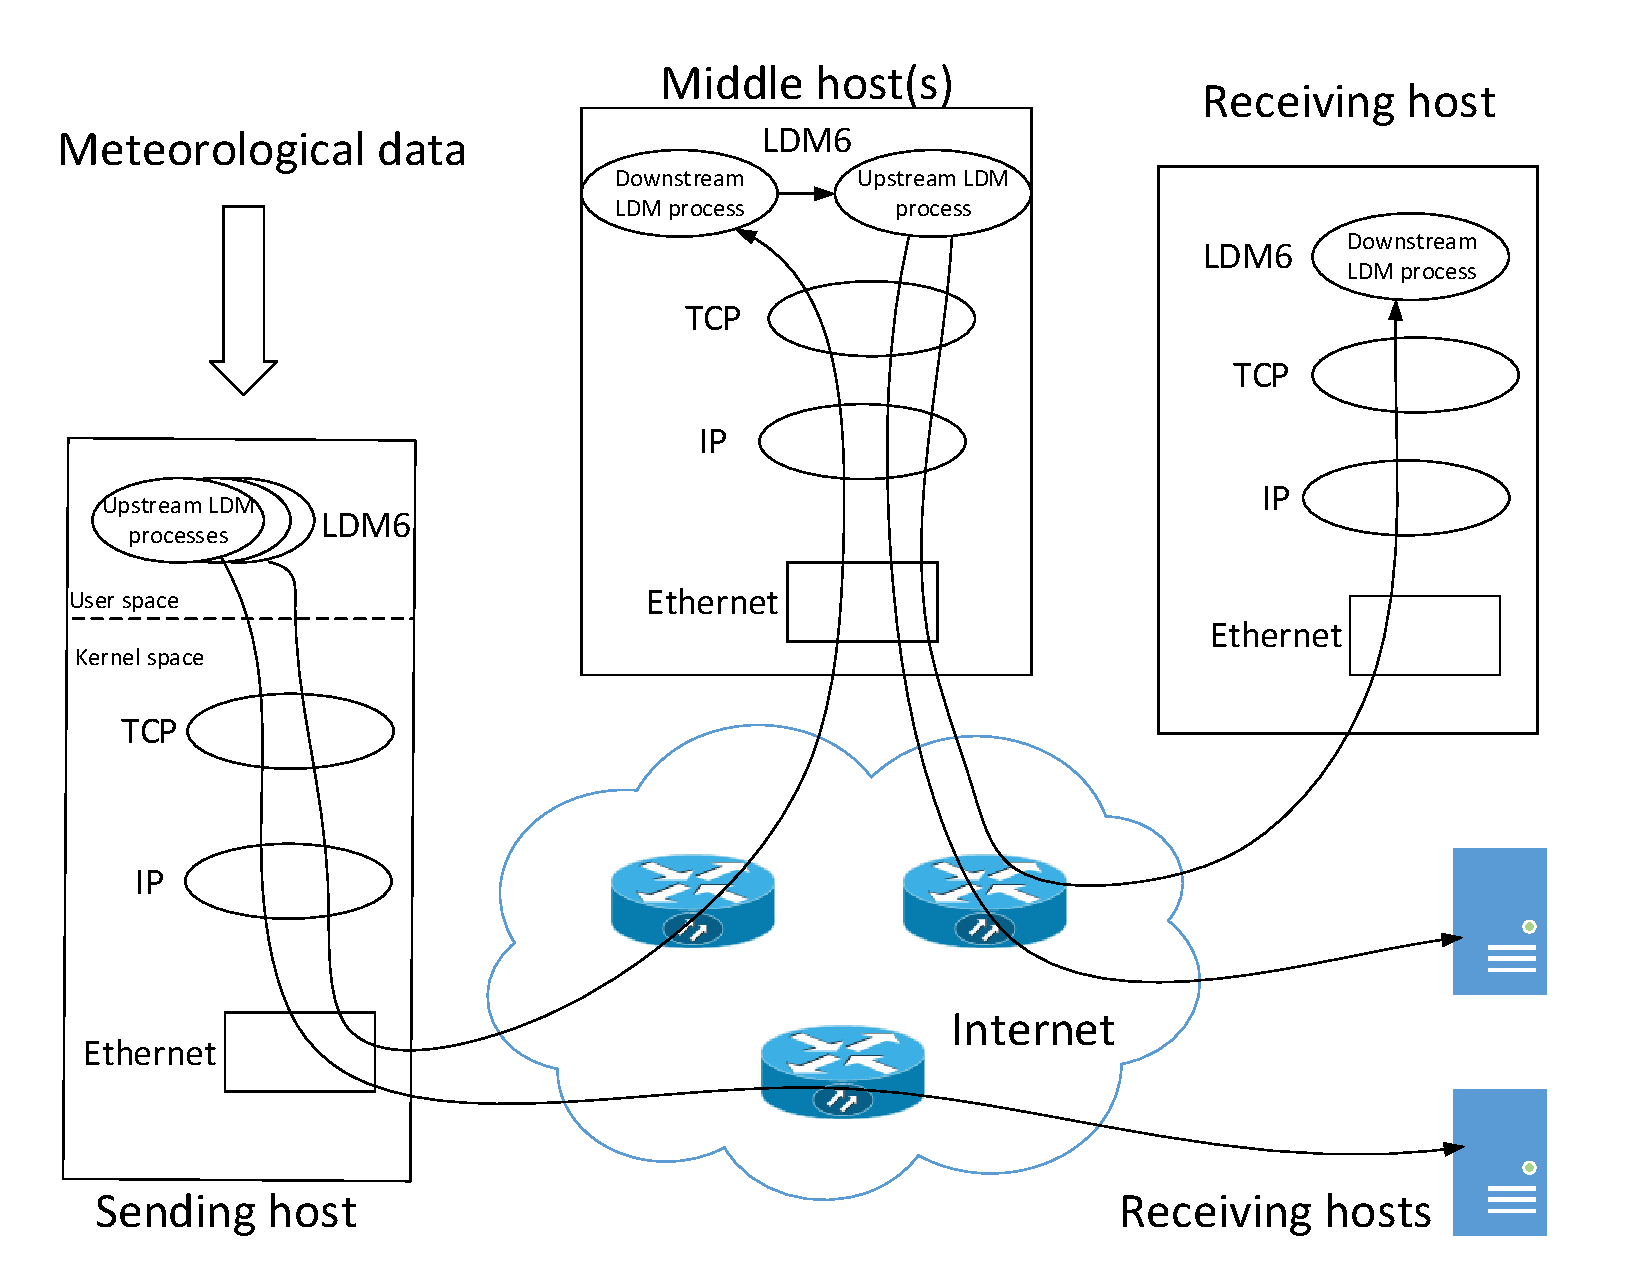
\includegraphics[width=0.60\textwidth]{figures/ALmulticast.pdf}
\caption{LDM6: Application-layer multicasting}
\label{fig:AL-multicast}
\end{figure*} 

\begin{figure*}[htbp!]
\centering
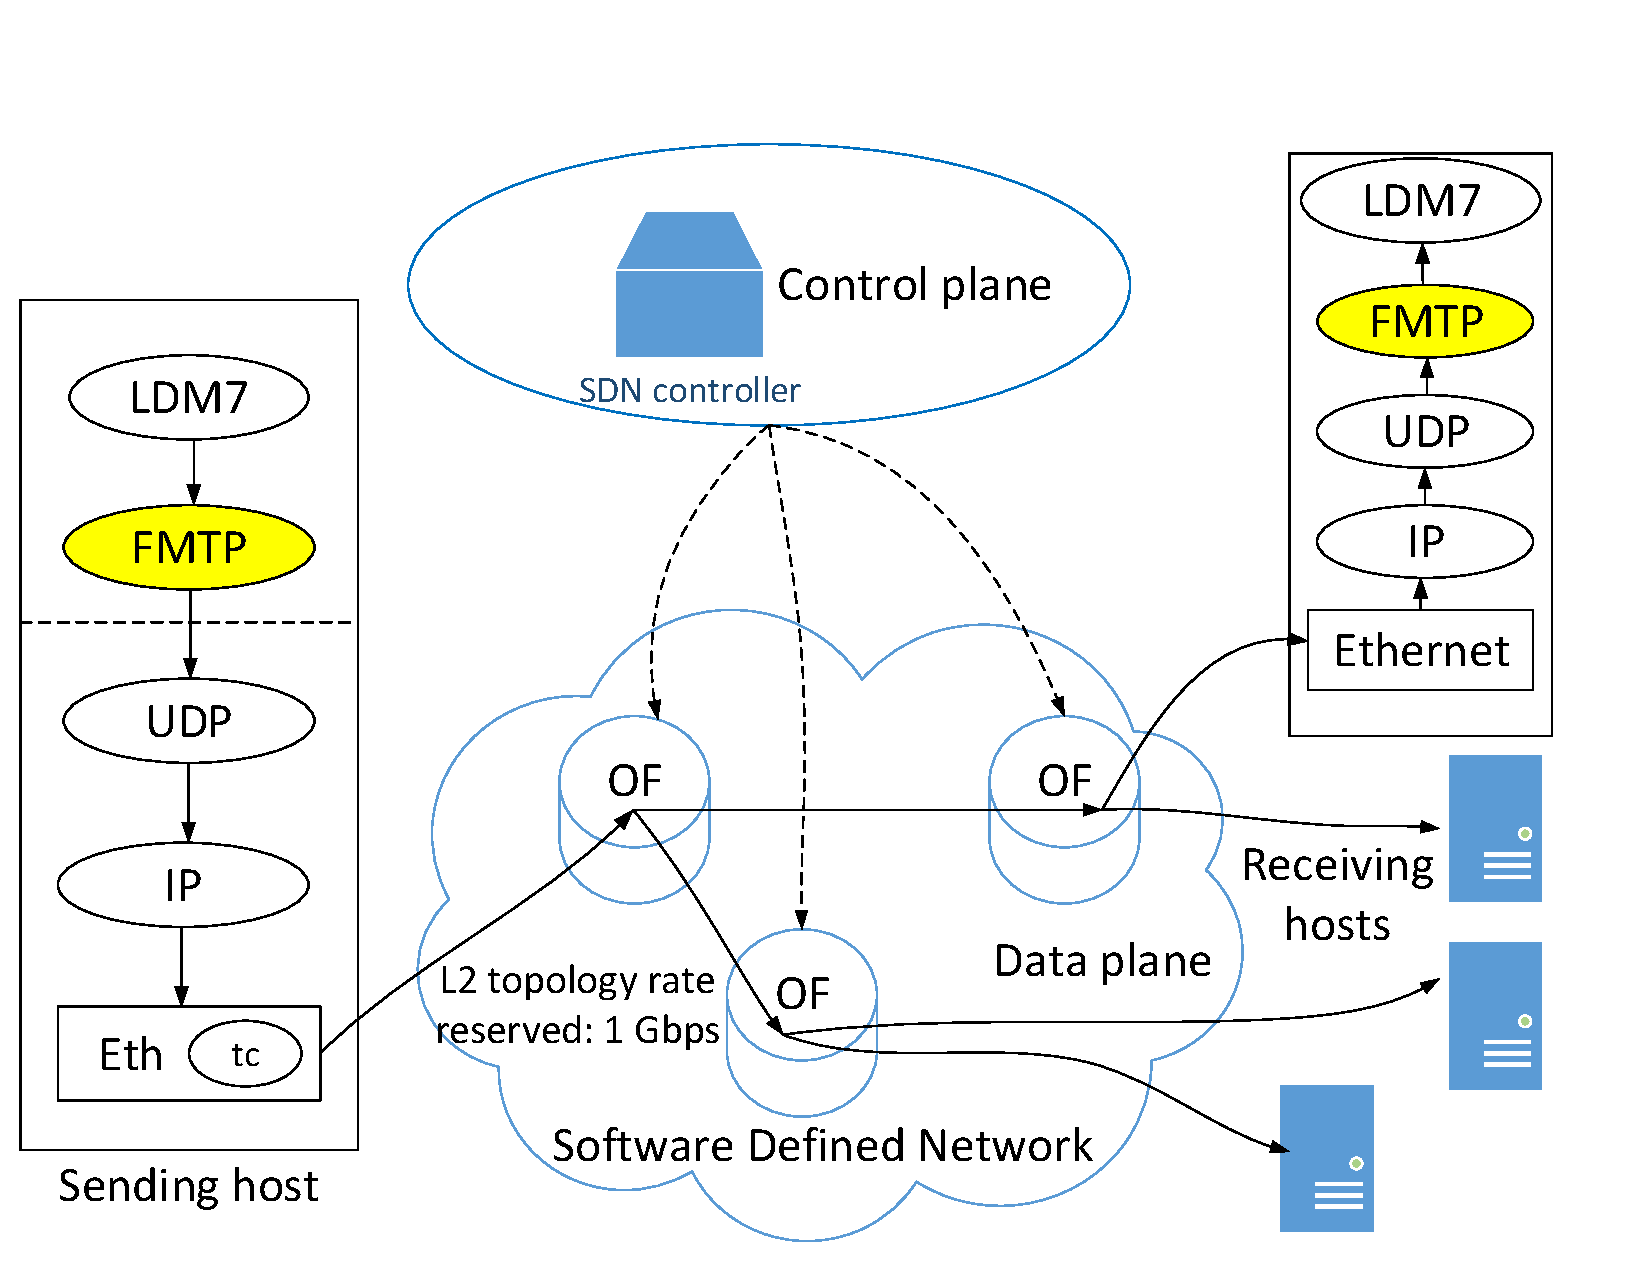
\includegraphics[width=0.60\textwidth]{figures/SDN.pdf}
\caption{LDM7: Layer-2 multicasting across an SDN}
\label{fig:SDN}
\end{figure*} 

\subsection{LDM7 solution for SDN: OpenFlow multicast}
\label{sec:LDM7}
The scalability problem can be solved by a solution in which network switches/routers perform the mulcasting action instead of servers. The availability of OpenFlow/SDN technologies has enabled the deployment of Layer-2 (L2) multipoint virtual topologies.There is a setup phase in which the SDN controller provisions the L2 virtual circuit. This phase is realized by OpenFlow control plane software,Open Exchange Software Suite (OESS) for intra-domain provision, and On-Demand Secure Circuits and Advance Reservation System (OSCARS) for inter-domain provision. Rate guarantees can be provided thus ensuring that there is no differential congestion levels on the paths from the sender to the multiple receivers. Therefore, the LDM7 which integrates the File Multicast Transport Protocol (FMTP) with the current version LDM is implemented for running over OpenFlow/SDN path-based virtual circuits networks, as shown in Fig.~\ref{fig:SDN}.

OpenFlow/SDN networks are now being deployed. For example,
Internet2, a core research-and-education network provider,
has deployed an Advanced Layer-2 Service (AL2S) on top of
a US-wide network of OpenFlow switches \cite{AL2S}.
Through an SDN controller, a multipoint L2 virtual topology can
be configured in the Ethernet switches to multicast Ethernet frames tagged with specific
Virtual LAN (VLAN) identifiers to multiple output ports. Comparing Figs~\ref{fig:AL-multicast} and \ref{fig:SDN}, we see that in the latter,
the OpenFlow switches are making copies of packets to multiple output
interfaces, unlike in the former, where the sending host and
middle hosts make the copies
at the application-layer (LDM6).
OpenFlow 1.3 supports
QoS features, which would allow for the L2 topology to be created with a specific
guaranteed rate. This concept is illustrated in Fig.~\ref{fig:SDN}.
The Linux \texttt{tc} (traffic control) utility can be used to set the rate
at which the Ethernet NIC transmits frames from the sending host. This rate
should be matched to the rate of the L2 multipoint virtual topology created by the
SDN controller. For example, if the NIC is 10 GE, but the rate used
in the setup phase is 1 Gbps, then the \texttt{tc} rate limit should be set to 1 Gbps.

Fig.~\ref{fig:SDN} shows the protocol layers between the application LDM7
and the Ethernet layer. File Multicast Transport Protocol (FMTP) is a reliable multicast transport protocol that we developed for use over rate-guaranteed L2 multipoint virtual topologies \cite{FMTP}.

As noted in Section~\ref{sec:intro}, there are silence periods between files
in the feedtypes. In other words, the file-streams are not continuous. Given
this traffic pattern,
it is challenging to determine an ideal rate for the L2 multipoint virtual topology. If the rate is too low, file-delivery latencies will be high.
If the rate is too high, then other requests for rate-guaranteed paths will be denied by the SDN controller. On the data-plane, QoS mechanisms for packet scheduling
allow the transmitter to send packets from other service classes during silence periods in the LDM file-streams. In other words, network resources are not being wasted during silence periods. This mode of
link sharing is called ``work conserving.'' Nevertheless, there is an incentive to choose a rate that is not too high, to accommodate other users' requests for rate-guaranteed paths. Therefore,
\emph{the problem statement of this thesis is to design a method for computing an ideal rate for the L2 multipoint virtual topology and the size for the buffer at the sending host given the characteristics of the file-stream, and latency and L2 path utilization goals.}
A buffer is used at the sending host to smooth out bursts of file arrivals. 


\section{Characterization of IDD feedtypes}
\label{sec:characterization}


We set up an LDM server on a host at the University
of Virginia (UVA) and configured the server to subscribe to just the
metadata (size and creation-time) for
the top five (from a  rate perspective) feedtypes \cite{IDD_Realtime}.
These are CONDUIT (\texttt{C}), NGRID (\texttt{NG}), NEXRAD2 (\texttt{N2}), NEXRAD3 (\texttt{N3}), and FSL2 (\texttt{F}).
Specifically, the \texttt{notifyme} utility was executed at the UVA LDM server
to receive the metadata for a week (June 2-8, 2014).
The \texttt{notifyme} utility allows a downstream LDM server to receive just the metadata about the files in a feedtype instead of the actual files.
The received metadata
was saved in log files. One entry row is saved in the log file
for each data product of each feedtype. The entry consists of the
creation-time when the product was injected into the IDD system for
distribution (which we refer to as ``arrival time''), and the product size.
The entries in the log files were sorted based on arrival time.
A Python script was implemented
to parse the metadata files and extract the size and arrival
instant of each data product (file).

\begin{table}[!ht]

\caption{Size (in KiB; unless otherwise stated) statistics; June 2, 2014; S: Skewness (R type-1); CV: Coefficient of Variation; M in size: MiB; K and M in last row: $10^3$ and $10^6$, respectively, for number of files.}
\label{tab:size-summary}
\begin{center}
    \begin{tabular}{|l|l|l|l|l|l|}     \hline
    \textbf{Size} & \textbf{\texttt{C}} &  \textbf{\texttt{NG}}  & \textbf{\texttt{N2}} & \textbf{\texttt{N3}} & \textbf{\texttt{F}}\\ \hline
    Min.                             & 0.17          & 0.06  		 & 0.1  		 & 0.15 		 & 0.21\\ \hline
    1st Q		        	      & 10       & 11.8 		& 35.33   		 & 5.18		 & 337.7\\ \hline
    Median                        & 26.7        & 30.3		& 56.3     	 & 9.3		 & 827.4\\ \hline
    Mean                           & 46.24        & 65.29 		& 71.24     	 & 18.88		 & 809.7\\ \hline
    3rd Q		               & 55.3        & 52.1		& 90.9  		 & 22.25		 & 1M\\ \hline
    Max                             & 510.2      & 23.7M    	& 498.5  	 & 206.7		 & 3M\\ \hline
    S		      & 3		 & 28.4	  	& 1.96	   	& 2.42		& 0.85\\ \hline
    CV			      & 1.3		  & 4.9	    	& 0.75	 	& 1.29		 & 0.75\\ \hline
    No.		      & 1.02M   &  526K 	& 1.02M   	& 1.02M	& 36K\\ \hline
\end{tabular}
\end{center}
\end{table}

\begin{table}
    \centering
      \caption{Inter-arrival time statistics; June 2, 2014} \label{tab:inter-arr-time-summary}
\begin{tabular}{|l|l|l|l|l|l|}     \hline
    \textbf{Time (ms)}            & \textbf{\texttt{C}} &  \textbf{\texttt{NG}}  & \textbf{\texttt{N2}} & \textbf{\texttt{N3}} & \textbf{\texttt{F}} \\ \hline
    Min.                             & 0        	   & 0 		& 0	 		 & 0	 		 & 0\\ \hline
    1st Q        	      & 0	           & 4 		& 15	   		 & 2			 & 7\\ \hline
    Median                        & 0	           & 10 		& 36		     	 & 4			 & 16\\ \hline
    Mean                           & 85      	  & 164 		& 85		     	 & 85			 & 2417 ms\\ \hline
    3rd Q                & 1	          & 23 		& 74   		& 11			 & 33\\ \hline
    Max                             & 3687s   & 68s    	& 2382s   	 & 2398s	 & 358s\\ \hline
    S		      & 301.2  & 23.1 	& 333.7   	& 271.3	& 11.6\\ \hline
    CV			      & 91.67  & 13.16    	& 53.10 	& 60.03	& 9.96\\ \hline
    \end{tabular}

\end{table}



\subsection{Size and inter-arrival time data}
\label{sec:size-arrtime}
Five IDD feedtypes are characterized 5 by making the histograms of size and inter-arrival time. We sort the data by ascending order and leave the 25\% data in the end so that the histograms present the distribution better.

% CONDUIT
\begin{figure}
\centering
    \begin{subfigure}{0.5\linewidth}
        \centering
        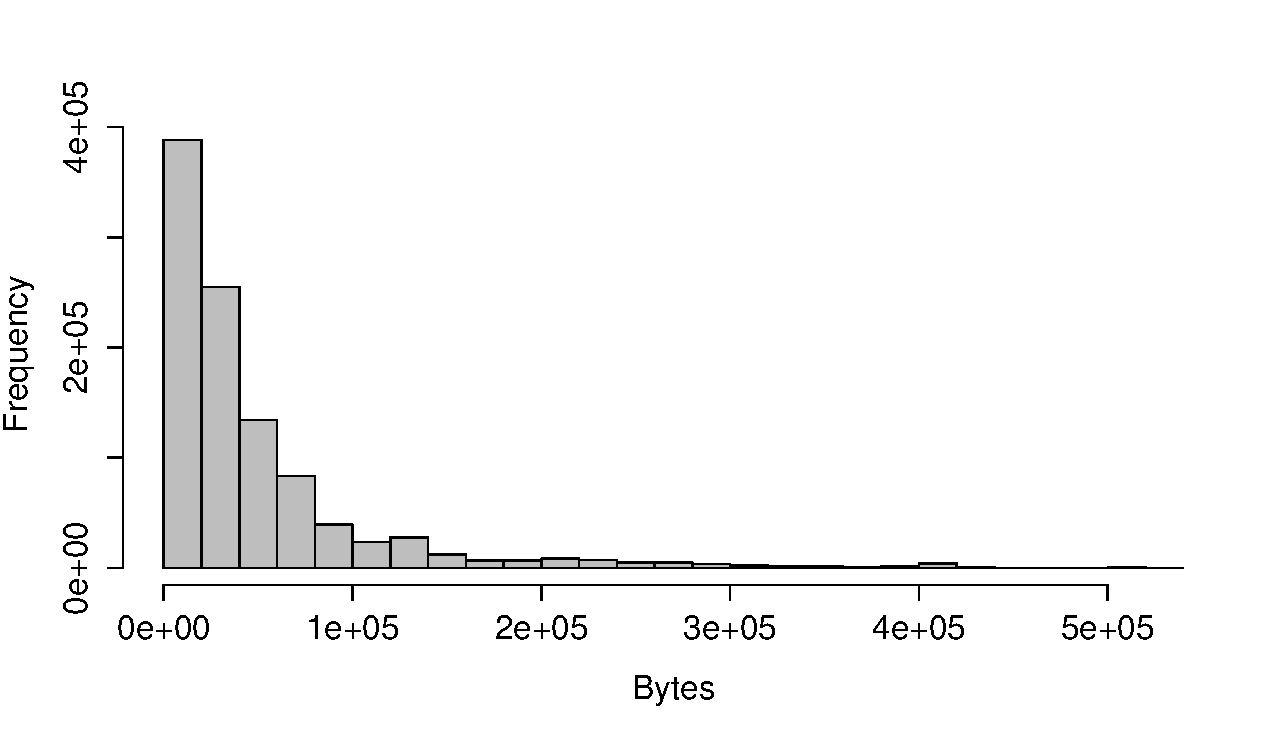
\includegraphics[width=2.2in]{figures/CONDUIT_20140602_Size_Hist.pdf}
        %\includegraphics[width=3.5in]{figures/CONDUIT_Size.eps}
        \caption{Whole size range; Count: 1017621}
        \label{CONDUIT_Size_Whole}
    \end{subfigure}\hfill
    \begin{subfigure}{0.5\linewidth}
	\centering
    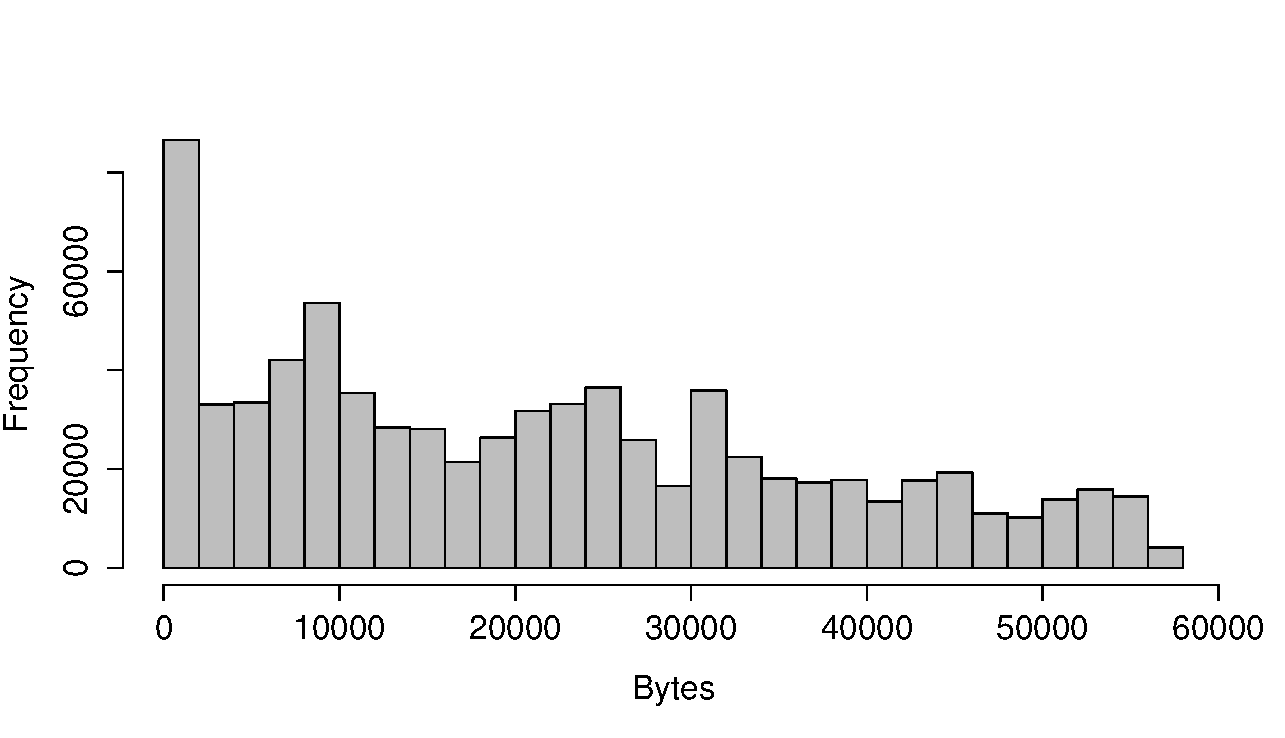
\includegraphics[width=2.2in]{figures/CONDUIT_20140602_Size_75percentile.pdf}
    %\includegraphics[width=3.5in]{figures/CONDUIT-size-75.eps}
        \caption{Top 75 percentile of size range; Count: 763216}
        \label{CONDUIT_Size_75}
    \end{subfigure}\hfill
\caption{Histogram of size of data products sent on June 02, 2014, for the CONDUIT feedtype}
    \label{CONDUIT_Size}
\end{figure}



For all the size and inter-arrival time of feedtypes, the distribution are highly right-skewed.
Fig.~\ref{CONDUIT_Size_75} zooms into the top 75\% data products (from a size perspective). Of the total number of data products, 1017621, as shown
in the last row of Table~\ref{tab:size-summary}, the number of products that fell in the range (0, 20000) bytes (B) was 388,228 (or 38\%). The largest size range (507, 510.2) KiB (1 KibiByte = 1024 B) had 25 data products.
The number of data products in the range (0, 2000) B is 86,520. In other words, 8.5\% of the products were
smaller than 2 KiB, and 38\% of the products were smaller than 20 KiB.

\begin{figure}
\centering
    \begin{subfigure}{0.5\linewidth}
        \centering
        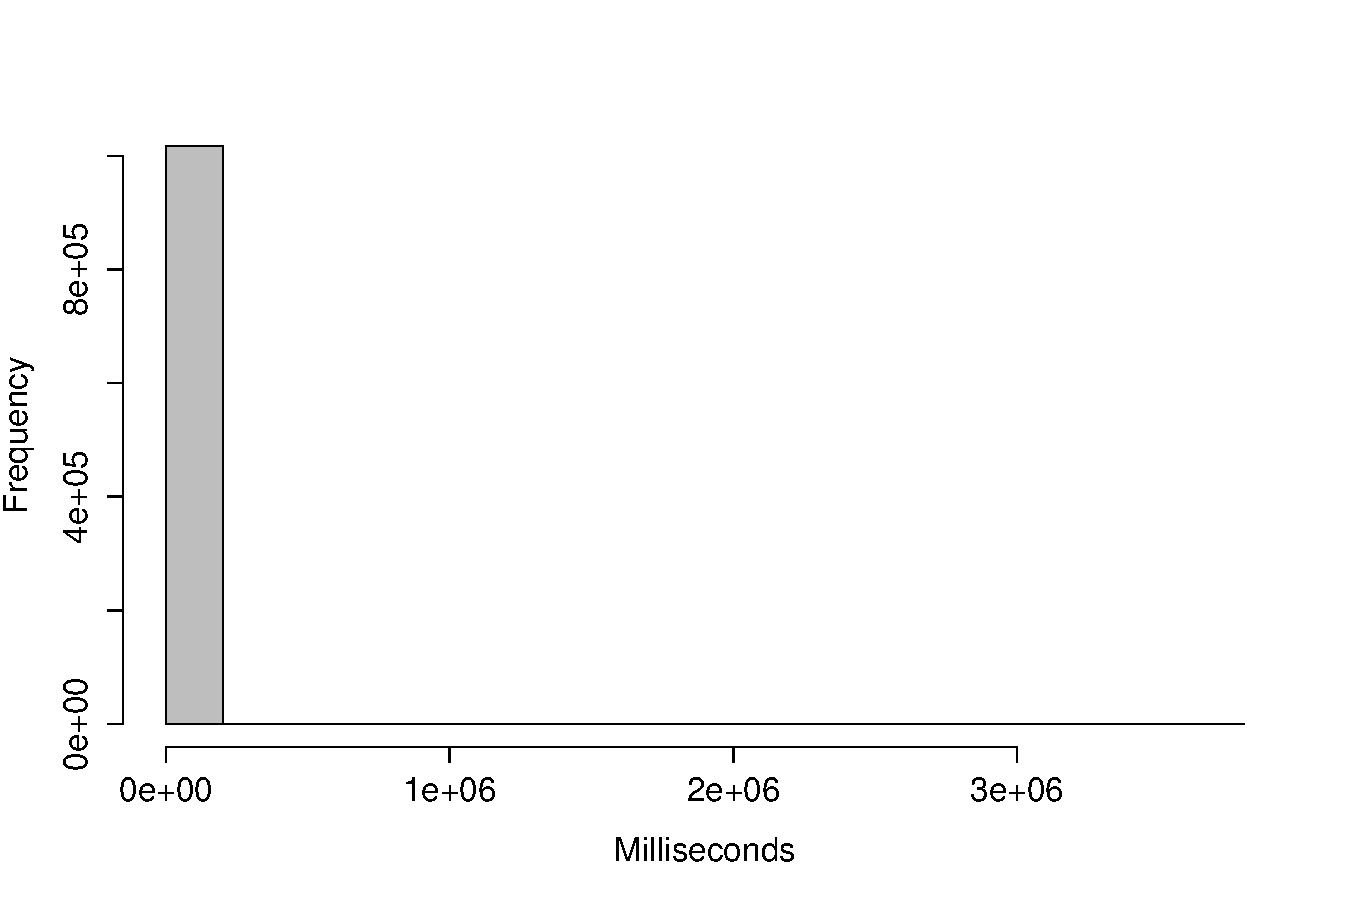
\includegraphics[width=2.2in]{figures/Inter-hist-CONDUIT0602.pdf}
        %\includegraphics[width=3.5in]{figures/CONDUIT_Size.eps}
        \caption{Whole inter-arrival time range; Count: 1017621}
        \label{CONDUIT_Inter_Whole}
    \end{subfigure}\hfill
    \begin{subfigure}{0.5\linewidth}
	\centering
    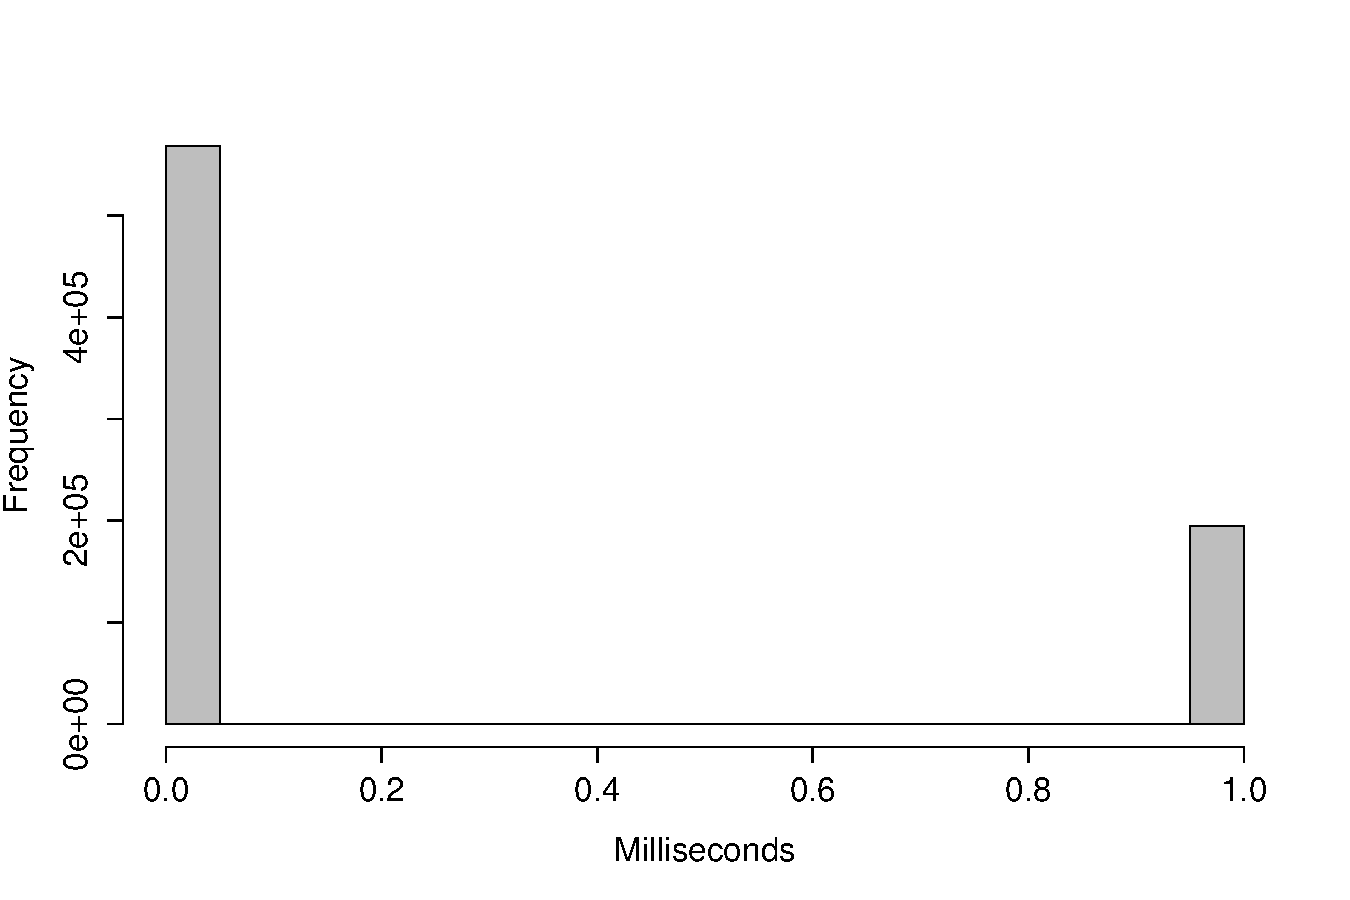
\includegraphics[width=2.2in]{figures/Inter-hist-CONDUIT0602-TOP75.pdf}
    %\includegraphics[width=3.5in]{figures/CONDUIT-size-75.eps}
        \caption{Top 75 percentile of inter-arrival time range; Count: 763216}
        \label{CONDUIT_Inter_75}
    \end{subfigure}\hfill
    \caption{Histogram of inter-arrival time of data products sent on June 02, 2014, for the CONDUIT feedtype}
    \label{CONDUIT_time}
\end{figure}

In the CONDUIT (\texttt{C}) feedtype, over 50\% of the products arrived in the same millisecond as their previous products, i.e., inter-arrival times for
these products was 0 ms (see Table~\ref{tab:inter-arr-time-summary}). Also, the maximum inter-arrival times were
quite large, e.g., maximum silence periods lasted more
than one hour for CONDUIT. (Also see per-min minute average rate figure of CONDUIT feedtype.)
Also, the Top 75\% inter-arrival time histogram indicates that over 25\% inter-arrival time are 1 millisecond.



Tables~\ref{tab:size-summary} and \ref{tab:inter-arr-time-summary} show statistics for sizes and inter-arrival times of data products
distributed in the five feedtypes on June 2, 2014. The NGRID (\texttt{N}) feedtype shows the most skewness for size (see Table~\ref{tab:size-summary}), and the inter-arrival time
coefficient of variation is high for all five feedtypes (see Table~\ref{tab:inter-arr-time-summary}).
Also the maximum-sized data product
is largest for the NGRID feedtype, while FSL2 (\texttt{F}) has the smallest number
of files and the files were generally larger than files in the other feed types.

For significant fractions of an hour
for NEXRAD2 (\texttt{N2}) and NEXRAD3 (\texttt{N3}). For example, as
CONDUIT data is generated by computer models,
this feedtype has silence periods when the models are not being executed.


\subsection{Rate data}
\label{sec:rate-results}
Fig.~\ref{fig:C-rate}, Fig.~\ref{fig:NG-rate}, Fig.~\ref{fig:N2-rate}, Fig.~\ref{fig:N3-rate}, Fig.~\ref{fig:FSL2-rate}  show a plot of per-min average rate, determined
by dividing the aggregate size of all files received in the minute by 60 sec,
as a function of time for 5 feedtypes. Both file-streams
show variable-rate arrivals. There are more silence periods and higher burstiness in the CONDUIT data than in the NGRID feedtype. 
The rate pattern for each day of the same feedtype is similar to each other. This finding is the basis for our problem statement of designing algorithms to determine the sending-host buffer size
and L2 virtual topology rate.

\begin{figure}
\centering
    \begin{subfigure}{0.5\linewidth}
        \centering
        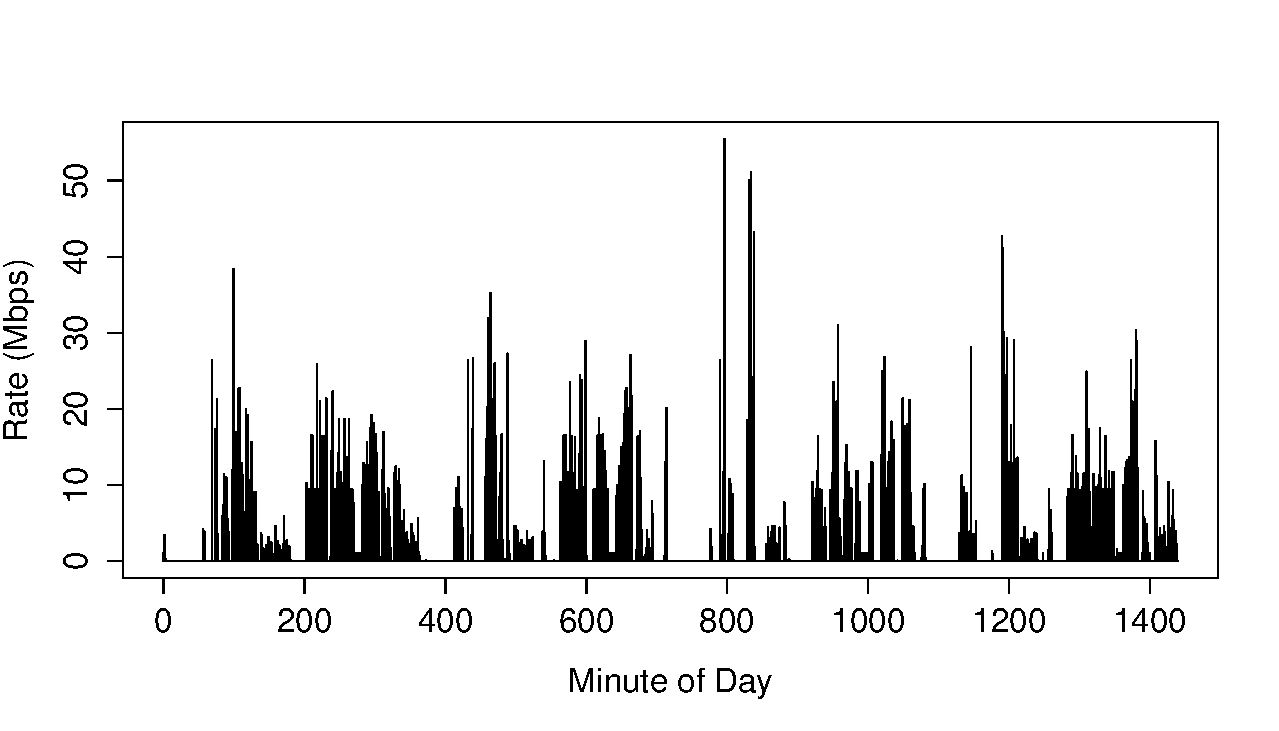
\includegraphics[width=2.2in]{figures/rate_time_CONDUIT0602.pdf}
        %\includegraphics[width=3.5in]{figures/CONDUIT_Size.eps}
        \caption{CONDUIT feedtype}
        \label{fig:C-rate}
    \end{subfigure}\hfill
    \begin{subfigure}{0.5\linewidth}
	\centering
    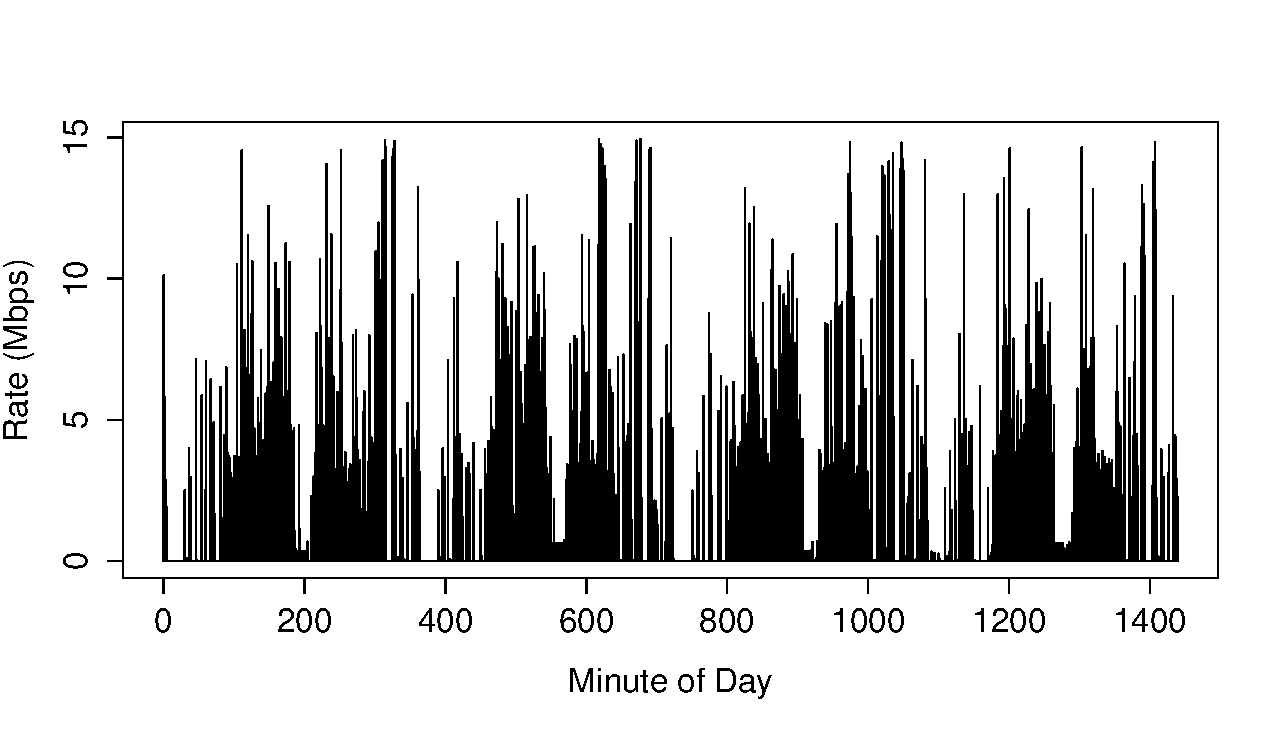
\includegraphics[width=2.2in]{figures/rate_time_NGRID0602.pdf}
    %\includegraphics[width=3.5in]{figures/CONDUIT-size-75.eps}
        \caption{NGRID feedtype}
        \label{CONDUIT_Inter_75}
    \end{subfigure}\hfill
    \caption{Rate vs. time of IDD feedtypes}
    \label{fig:NG-rate}
\end{figure}








\section{Rate selection algorithms for LDM7}
In Section~\ref{sec:LDM7}, we noted that LDM7 is currently
under development, and is designed to use software defined networks.
Further details of
this solution are described in this section.

Fig.~\ref{fig:software} illustrates the LDM7
architecture and operation. The LDM7 server sending host receives
meteorological data at a variable rate. Therefore, we use
a buffer of size $B$ to hold files as the lower protocol layers
(see Fig.~\ref{fig:SDN} for details) divide the files into blocks
and send them to the Ethernet NIC for transmission. The Linux \texttt{tc}
utility is configured to send data at rate $R$, which is equal to the rate
used by the SDN controller to establish the L2 multipoint virtual
topology.

The downstream LDM7 processes are configured to save metadata about the files in a feedtype while receiving the actual files. The metadata is saved in log files. Periodically,
the LDM7 controller shown in Fig.~\ref{fig:software}
reads the log files collected by the receivers, and runs an algorithm,
which is described in Section~\ref{sec:algorithm} to determine the
buffer size $B$ and rate $R$. If the newly computed rate is different
from the rate of the existing L2 multipoint virtual topology, the LDM7 controller
sends a request to the SDN controller to modify the L2 multipoint
virtual topology rate.
Additionally, the LDM7 controller sends a control-plane
message to the LDM7 server in the sending host to reconfigure the Linux \texttt{tc} settings to use the new $R$ value. If the buffer size $B$
also changes, the new buffer size is sent by the LDM7 controller to the sending host as shown in Fig.~\ref{fig:software}.

\begin{figure}
\centering
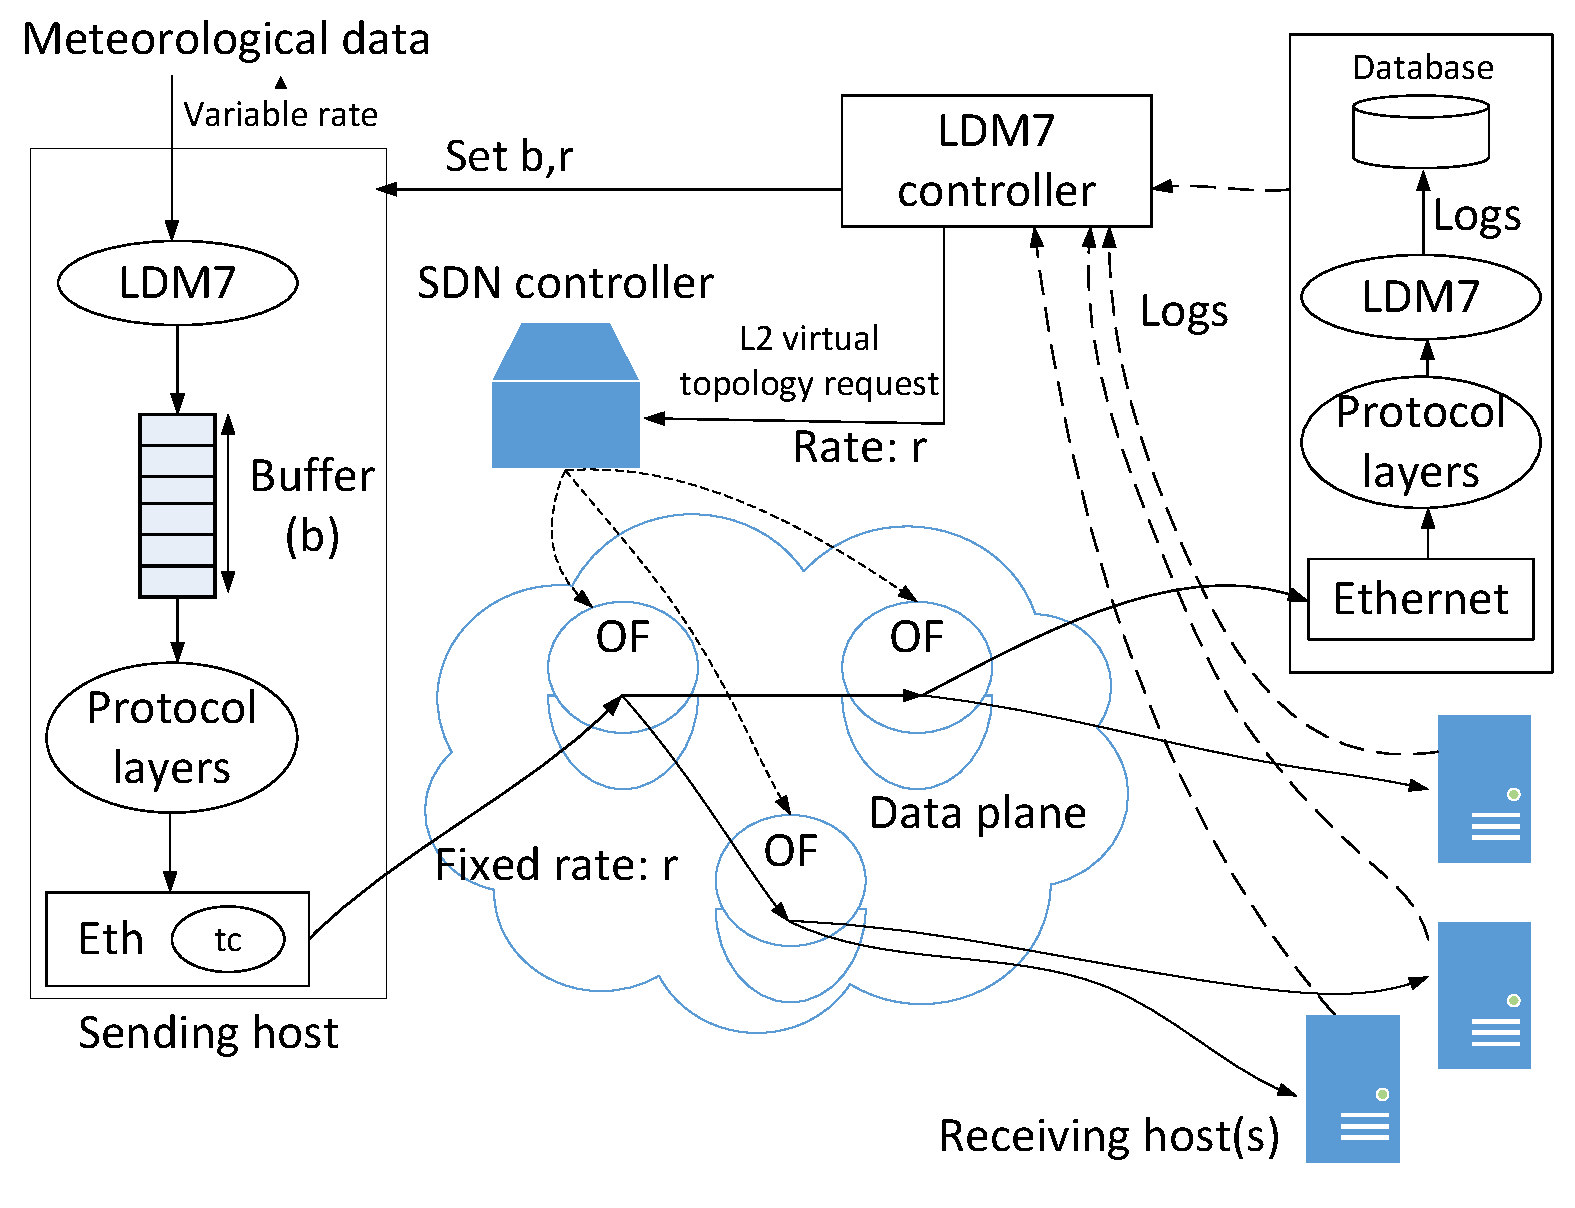
\includegraphics[width=0.5\textwidth]{figures/software.pdf}
\caption{LDM7 architecture and operation}
\label{fig:software}
\end{figure}

\subsection{Algorithms}
\label{sec:algorithm}
The \emph{objective} of the algorithm is to select a rate for the L2 multipoint virtual topology, and a size for the sending-side
buffer, given certain constraints. These constraints are
determined by the method used in the upstream LDM server for
scheduling file transmissions. Since inter-arrival times are short
(see Table~\ref{tab:inter-arr-time-summary}), the upstream LDM
server could be programmed to use of several options for  multiplexing
file transmissions.

In this thesis, we consider two modes: (i) Round Robin (RR), and
(ii) First-Come First Served (FCFS). In RR mode, as new files
arrive, they are immediately added to the buffer, and files in the
buffer are served out one packet at a time.
In FCFS mode, each file is fully transmitted before the next file is served.
In the RR mode, a threshold
$(\mathbb{G},\beta)$ is set such that only
a $\beta$ fraction of files experience multicast throughput less than $\mathbb{G}$.
In the FCFS mode, a wait-time threshold $(\mathbb{W},\alpha)$ is set such that only an $\alpha$ fraction of files experiences a wait time greater than $\mathbb{W}$.

\subsubsection{Overview}

The algorithm
is described for computing and rate and buffer for a single feedtype.
Table~\ref{tab:notation} describes the notation used.
\begin{table*}[!ht]
\centering
\caption{Notation}
\begin{tabular}{|l|p{12.5cm}|}
\hline
\multicolumn{2}{|c|}{Input parameters}\\ \hline
$i$ and $j$ & file indexes\\ \hline
$(t,t+k\tau)$ & $k^{th}$ holding interval \\ \hline
$a_i$ & arrival time of file $i$ \\ \hline
$s_i$ & size of file $i$\\ \hline
\multicolumn{2}{|c|}{System parameters}\\ \hline
$(\mathbb{G},\beta)$ & Fraction $\beta$ of files can experience multicast throughput less than $\mathbb{G}$ in RR mode\\ \hline
$(\mathbb{W},\alpha)$ & Fraction $\alpha$ of files can experience wait times greater than $\mathbb{W}$ in FCFS mode\\ \hline
$r_k$ & configured rate used in the $k^{th}$ holding interval\\ \hline
$b_k$ & configured buffer size used in the $k^{th}$ holding interval \\ \hline
\multicolumn{2}{|c|}{Intermediate values}\\ \hline
$R_k$ & ideal computed rate for the $k^{th}$ holding interval\\ \hline
$B_k$ & ideal computed buffer size for the $k^{th}$ holding interval \\ \hline
$q(t)$ & sending-host buffer (queue) occupancy at time $t$ in ideal case \\ \hline
%$n(t)$ & number of files in the sending-host buffer at time $t$ in ideal case \\ \hline
$d_i$ and $d^{\prime}_i$  & departure time of file $i$, actual and ideal, respectively\\ \hline
$w_i$ and $w^{\prime}_i$ & FCFS wait time experienced by file $i$, actual and ideal, respectively \\ \hline
$g_i$ and $g^{\prime}_i$ & multicast file-transfer throughput of file $i$, actual and ideal, respectively\\ \hline
$\textbf{A}_k$ & set of files that arrived in the $k^{th}$ holding interval \\ \hline
$\textbf{D}_k$ and $\textbf{D}^{\prime}_k $& set of files that departed in the $k^{th}$ holding interval, actual and ideal, respectively \\ \hline
$N_k$ and $N^{\prime}_k $ & number of files that arrived and departed in the $k^{th}$ holding interval, actual and ideal, respectively \\ \hline
$\textbf{M}_k$ and $\textbf{M}^{\prime}_k $ & RR: set of files that experienced multicast throughput lower than $\mathbb{G}$, actual and ideal, respectively\\ \hline
$\textbf{V}_k$ and $\textbf{V}^{\prime}_k $ & FCFS: set of files that experienced wait times greater than  $\mathbb{W}$, actual and ideal, respectively\\
\hline
$\textbf{L}_k$ & set of files that were dropped due to lack of space in the sending-host buffer in the $k^{th}$ holding interval \\ \hline
\multicolumn{2}{|c|}{Output metrics}\\ \hline
$U_k$ & path utilization in the $k^{th}$ holding interval \\ \hline
$\Theta_k$ & mean multicast throughput of files that arrived and departed  in the $k^{th}$ holding interval\\ \hline
$\delta_k$ & dropped file rate in the $k^{th}$ holding interval\\ \hline
$\eta_k$ & RR: throughput-violation rate in the $k^{th}$ holding interval\\ \hline
$\gamma_k$  & FCFS: waiting-time violation rate in the $k^{th}$ holding interval\\ \hline
\end{tabular}
\label{tab:notation}
\end{table*}




First we define a term called \emph{Holding interval}, which is the
period for which the assigned rate and buffer size (as illustrated in
Fig.~\ref{fig:software}) are held unchanged. The $k^{th}$ holding interval is
denoted $(t,t+k\tau)$ in Table~\ref{tab:notation}. The arrival time and
size of file $i$ are denoted $a_i$ and $s_i$, respectively. The file index $i$ is reset to 1 for the first file arriving in each holding interval.

The sizes and arrival times
of all files that arrived and departed in the holding interval are used
to compute the ideal (post-facto) rate $R_k$ and buffer size $B_k$ that should have been used for the $k^{th}$ holding interval, given
the $(\mathbb{G},\beta)$ and $(\mathbb{W},\alpha)$
thresholds, for the RR and FCFS schemes, respectively. The
ideal rate $R_k$ and buffer size $B_k$ values are combined with the current
rate $r_k$ and buffer size $b_k$ that are in use in the $k^{th}$ holding interval to determine rate $r_{k+1}$ and buffer size $b_{k+1}$
for use in the $(k+1)^{th}$ holding interval.
In other words this solution is an empirical method
for determining the rate and buffer size based on traffic characteristics. An Exponential Weighted
Moving Average (EWMA) scheme such as that used for TCP Round-Trip Time (RTT) estimation to compute Retransmission Time Out (RTO) at the TCP sender is used here to modify the rate/buffer setting from one holding
interval to the next.

Table~\ref{tab:notation} lists the thresholds, $(\mathbb{G},\beta)$ and $(\mathbb{W},\alpha)$, and the configured rate $r_k$ and buffer size $b_k$ as system parameters. Next, Table~\ref{tab:notation} lists a number of intermediate values
computed by the algorithm, and the output metrics.
The reader is referred
to Table~\ref{tab:notation} for details of these values
and metrics.

In the next three subsections~\ref{sec:buffer}, \ref{sec:rate-RR}, and \ref{sec:rate-FCFS},
we describe how the ideal buffer size  $B_k$ and ideal rate $R_k$
can be computed post-facto, i.e., with knowledge of sizes and
arrival times of all files received within a holding interval
$(t,t+k\tau)$. Subsection~\ref{sec:output} describes how
the output metrics are computed, and finally Subsection~\ref{sec:EWMA} shows how the rate and buffer
size settings for the next holding interval are set.

\subsubsection{Ideal buffer size computation}
\label{sec:buffer}

Buffer size can be specified using the same notation for both RR and FCFS modes. Using an ideal path rate $R_k$, buffer occupancy at the time of arrival of each
file is as follows:
\begin{eqnarray}
q(a_1) & = & q(t+(k-1)\tau) \nonumber \\
q(a_2) & = & \max\{0, q(a_1)+s_1 - R_k \times (a_2 -a_1)\} \nonumber \\
q(a_i) & = & \max\{0, q(a_{i-1}) +s_{i-1} - R_k \times (a_i -a_{i-1})\}
\end{eqnarray}
The buffer occupancy at the time of arrival of the first file
of the $k^{th}$ holding interval is the buffer occupancy at the starting instant of
the holding interval, which is $(t,t+(k-1) \tau)$.
The buffer would be drained at rate $R_k$ and hence at the time of arrival
of the second file $a_2$, the buffer is either empty, or has some leftover
bytes from the previous files if those files could not be served out completely before the second file of the $k^{th}$ holding interval arrived. Similar reasoning can be
applied to the buffer occupancy at the time of arrival of an arbitrary
file $i$.

To ensure 0 loss in the $k^{th}$ holding interval, the buffer size $B_k$ should ideally be
\begin{equation}\label{eqn:ideal-buffer}
B_k = \max_{1 \leq i \leq \left\vert\textbf{A}_k\right\vert)} q(a_i)
\end{equation}
where $\textbf{A}_k$ is the set of files that arrived in the
$k^{th}$ holding interval as shown in Table~\ref{tab:notation}. The ideal buffer size $B_k$ depends
on the ideal path rate $R_k$, which in turn is selected for the two modes,
RR and FCFS, as described in the next two subsections, respectively.

\subsubsection{Ideal path rate computation in RR mode}
\label{sec:rate-RR}
The algorithm starts with a configured initial value for $R_k$.
If this value is too small, then the minimum multicast throughput
threshold $\mathbb{G}$ will not be met for at least $(1-\beta)$ fraction of the files. Therefore the algorithm keeps increasing $R_k$ until
$(\mathbb{G},\beta)$ is met.
If the starting value chosen for $R_k$ is too large, and this threshold is not exceeded, the algorithm will
keep decreasing $R_k$ until this threshold is violated. In other words, the algorithm finds the minimum $R_k$ value while simultaneously ensuring that not more than a $\beta$ fraction of the files experience a multicast throughput less than $\mathbb{G}$.

The departure times, $d^{\prime}_i$, assuming the ideal
rate and buffer size can be computed by having the algorithm
track packet emission delays. With these departure times,
the ideal multicast file-transfer throughput for file $i$ would be
\begin{equation} \label{eqn:file-throughput}
g^{\prime}_i = \frac{s_i}{(d^{\prime}_i - a_i)}
\end{equation}

Ideal path rate $R_k$ for the $k^{th}$ holding interval is the smallest value at which the following inequality holds:
\begin{equation} \frac{\left\vert{\textbf{M}^{\prime}_k}\right\vert}{N^{\prime}_k}  \le \beta
\end{equation}
where $i \in \textbf{M}^{\prime}_k$ if $g^{\prime}_i < \mathbb{G}$
and $t \leq a_i, d^{\prime}_i \leq t+k\tau$.
The set of files that would have experienced multicast throughput lower than $\mathbb{G}$ in the $k^{th}$ holding interval is $\textbf{M}^{\prime}_k$, and $N^{\prime}_k$ is the number of
files that would have arrived and departed in the $k^{th}$ holding interval, under ideal assumptions of rate and buffer size.
$N^{\prime}_k = \left\vert\textbf{A}_k \cap \textbf{D}^{\prime}_k\right\vert$.


\subsubsection{Ideal path rate computation in FCFS mode}
\label{sec:rate-FCFS}
Each newly arriving file $i$ will experience a waiting
time that is dependent on the buffer occupancy at the time of its arrival $a_i$,
and the ideal path rate $R_k$, since, in
FCFS mode, each file is transmitted in its entirety before
the next file is served.
Thus, waiting time for file $i$ in FCFS mode is:
\begin{equation} \label{eqn:ideal-wait}
w^{\prime}_i = \frac{q(a_i)}{R_k}
\end{equation}
Ideal path rate $R_k$ for the $k^{th}$ holding interval is the smallest value
at which the following inequality holds:
\begin{equation}
\frac{\left\vert\textbf{V}^{\prime}_k\right\vert}{N^{\prime}_k} \leq \alpha
\end{equation}
where $i \in \textbf{V}^{\prime}_k$ if $w^{\prime}_i < \mathbb{W}$
and $t \leq a_i, d^{\prime}_i \leq t+k\tau$.
The set of files that would have experienced wait times in the sending-host buffer greater than $\mathbb{W}$  in the $k^{th}$ holding interval is $\textbf{V}^{\prime}_k$ under ideal assumptions of rate and buffer size.

In FCFS mode, the ideal departure time for file $i$ would be
\begin{equation}\label{eqn:FCFS-wait}
d^{\prime}_i= (w^{\prime}_i + s_i/R_k) + a_i
\end{equation}
where $w^{\prime}_i$ is given by \eqref{eqn:ideal-wait}.

\subsubsection{Output measures}
\label{sec:output}

Five output measures are considered: (i) mean multicast throughput,
(ii) L2 multipoint virtual topology utilization, (iii) dropped-file
rate, (iv) RR: throughput-violation rate and (v) FCFS: waiting-time violation rate. The output measures under the actual rate $r_k$ and
buffer size $b_k$ used in the $k^{th}$ holding interval are computed
below.

The multicast file-transfer throughput for file $i$ is given by
\begin{equation} \label{eqn:file-throughput}
g_i = \frac{s_i}{(d_i - a_i)},
\end{equation}
where $d_i$, the departure time of file $i$, is computed
under RR and FCFS mode assumptions using the actual rate and buffer
size. For example, under FCFS mode, $d_i$ is computed
using \eqref{eqn:FCFS-wait} with
the actual rate $r_k$ instead of the ideal rate $R_k$,
and with $w^{\prime}_i$ replaced by $w_i$, which can be computed
using \eqref{eqn:ideal-wait} but with $r_k$ instead of $R_k$.

The mean multicast throughput for the files that arrived and departed in the $k^{th}$ holding interval is:
\begin{equation}
\Theta_k = \frac{1}{N_k} \sum_{i=1}^{i=N_k} g_i
\end{equation}
where $N_k$ is the actual number of files that arrived and
departed in the $k^{th}$ holding interval, i.e.,
$N_k = \left\vert\textbf{A}_k \cap \textbf{D}_k\right\vert$.
We use the term ``multicast throughput'' instead of the term
``throughput'' as the latter should reflect time for retransmissions,
if any. Packet loss, which can occur at the receiver buffers
even in rate-guaranteed networks, and the corresponding mechanism for retransmssions, are addressed in our reliable multicast transport protocol \cite{FMTP}.

The path utilization in the $k^{th}$ holding interval is given by:
\begin{equation} \label{eqn:util}
U_k \approx \frac{\sum_{i=1}^{i=N_k} s_i}{r_k \times \tau}.
\end{equation}
In other words, utilization is the fraction of time that the path is in use. The reason for the approximate sign is that some parts of the files that were in the sending-side buffer at time $(t+(k-1)\tau)$ (start of the
$k^{th}$ holding interval), and parts of the files that remain in the buffer at time $(t+k\tau)$ (end of the $k^{th}$ holding interval),
would also have been served during
that interval, and therefore the utilization will be greater than
estimated by \eqref{eqn:util}. The longer the holding interval the more
accurate the approximation.

If there is insufficient space in the sending-host buffer to hold file $i$ at the time of its arrival $a_i$, then the file will be dropped, i.e., if
$q(a_i) + s_i > b_k$, the file index $i$ is added to set
$\textbf{L}_k$. Dropped file rate in the $k^{th}$ holding interval is:
\begin{equation}
\delta_k = \frac{\left\vert\textbf{L}_k\right\vert}{N_k}
\end{equation}
With the ideal rate and buffer values
($R_k$ and $B_k$), there will 0 dropped files because the ideal buffer size was selected using \eqref{eqn:ideal-buffer}, but with the actual rate and
buffer settings ($r_k$ and $b_k$), a file will be dropped if
there is insufficient space in the buffer to hold the file
at the time of its arrival.

Similarly with the ideal rate and buffer values, the $(\mathbb{G},\beta)$ and $(\mathbb{W},\alpha)$ thresholds for RR and FCFS, respectively,
will not be violated because these thresholds were considered while determining
the ideal values. However, with the actual rate and buffer size, these thresholds could be violated.
Using sets $\textbf{M}_k$ and $\textbf{V}_k$ to represent the
set of files that experienced multicast throughput lower than $\mathbb{G}$ in the RR mode, and experienced
wait times greater than $\mathbb{W}$ in the FCFS mode, respectively,
we define the RR-mode throughput
violation rate $\eta_k$ and FCFS-mode waiting-time violation rate $\gamma_k$.

RR-mode throughput violation rate is:
\begin{equation}
\eta_k = \frac{\left\vert\textbf{M}_k\right\vert}{N_k}
\end{equation}

FCFS-mode waiting-time violation rate is:
\begin{equation}
\gamma_k = \frac{\left\vert\textbf{V}_k\right\vert}{N_k}
\end{equation}

\subsubsection{EWMA procedure to compute actual rate and buffer size}
\label{sec:EWMA}

An empirical approach is used to compute the L2 multicast path
rate and sending-host buffer size based on the observed metadata
in each holding interval.
Using EWMA, controlled with a weight parameter $W$, the rate used
in the $(k+1)^{th}$ holding interval, $r_{k+1}$ is computed from
the rate  $r_{k}$ used in the $k^{th}$ holding interval, and the ideal
rate, $R_k$, computed for the $k^{th}$ holding interval, as follows:
\begin{equation}\label{eqn:EWMA}
r_{k+1} = \frac{W}{(W+1)} r_k + \frac{1}{(W+1)}  R_k
\end{equation}

%Using EWMA with a weight factor of $\alpha$,
%\begin{equation}
%b_{k+1} = (1-\alpha) b_k + \alpha B_k
%\end{equation}

For the buffer size at the sending host, it is important to
keep dropped-file rate as close to 0 as possible. Therefore,
our approach is to choose the bigger of two values, the buffer
size, $b_k$, used in the $k^{th}$ holding interval, and the newly
computed ideal buffer size, $B_k$, for the buffer size for the next
holding interval. Therefore:
\begin{equation}
b_{k+1} = max(B_k,b_k)
\end{equation}
Administrative procedures can be used to monitor the $b_k$ value
and lower the buffer size if the ideal buffer size computed
on several consecutive holding intervals is considerably lower. 



\section{Numerical results}
The one-week data for the five feedtypes characterized
in Section~\ref{sec:characterization} is used for an application
of the algorithm described in Section~\ref{sec:algorithm}.
Section~\ref{sec:rate-buffer}
shows results
obtained by applying the ideal buffer-size and ideal
rate computation methods, described in Sections~\ref{sec:buffer} and \ref{sec:rate-RR} for the RR-mode,
to one-day's data (holding interval is 1 day) for the five feedtypes. 
Section~\ref{sec:FCFS-RR-comparison} discusses the differences
in results obtained for the ideal buffer size and rate
under the assumptions of RR mode and FCFS mode.
The output metrics, as described in Section~\ref{sec:output},
are presented. Section~\ref{sec:EWMA-results}
presents results for the CONDUIT feedtype
when applying the EWMA method
described in Section~\ref{sec:EWMA} for six consecutive days.

\subsection{Computing ideal rate and buffer size for RR mode}
\label{sec:rate-buffer}

We used threshold values, $\mathbb{G}=10$ kbps, $\beta=0.05$,
to run the RR-mode algorithm first and found the minimum path
rate and buffer size for each of the five
feedtypes using the June 2, 2014 metadata.
Table~\ref{tab:RR-rate-buffer} shows the results.
\begin{table}
\caption{June 2, 2014; Ideal path rate and buffer size in RR mode; $\mathbb{G}=10$ kbps; $\Theta$: mean multicast throughput; $\beta=0.05$}
\centering
\begin{tabular}{| c | p{0.5in} | p{0.4in} | p{0.3in} |p{0.6in}|} \hline
Feedtype & Rate (Mbps) & Buffer size (MiB) & Util. (\%) & $\Theta$ (kbps)\\ \hline
CONDUIT & 36 & 248 & 12.4 & 535.2 \\ \hline
NGRID &10 & 315 & 32.6 &436.6  \\ \hline
NEXRAD2 & 16& 38 &42.9 &7370.2   \\ \hline
NEXRAD3 &6 & 19 &30.4 &661.6 \\ \hline
FSL2 & 4 & 306 &68.6 &54.4  \\ \hline
% FSL2 (G=20) & 6 &244 &45.7&119.3  \\ \hline
\end{tabular}
\label{tab:RR-rate-buffer}
\end{table}
The ideal rate computed for the CONDUIT feedtype is 36 Mbps,
and the ideal buffer size is 248 MiB. Had these rate and buffer
settings been used, no files would have been dropped.

The utilization and mean multicast throughput values shown
in Table~\ref{tab:RR-rate-buffer} are computed using the methods
described in Section~\ref{sec:output} but with the ideal rate and buffer
size settings, not the actual rate and buffer size settings as described
in that section. In other words, the mean multicast throughput across the 1.02 M files (see last row
of Table~\ref{tab:size-summary}) received that day for the CONDUIT feedtype
would have been 535.2 kbps had the ideal rate and buffer settings been used. The L2 multicast path would have been
only utilized at only 12.4\%.
As noted in Section~\ref{sec:LDM7}, utilization is not a concern per-se
because the link is shared in work-conserving mode. The CONDUIT traffic
is bursty (see Fig.~\ref{fig:C-rate}), and therefore, 36 Mbps is the smallest rate at which the
$(\mathbb{G},\beta)$ threshold values can be met. On the other hand,
the utilization of a 4 Mbps path is 68.6\% for the FSL2 feedtype
as seen in the last row of Table~\ref{tab:RR-rate-buffer}.

\subsection{Comparing the two modes, RR and FCFS}
\label{sec:FCFS-RR-comparison}
We executed the FCFS-mode algorithm described in Sections~\ref{sec:buffer} and ~\ref{sec:rate-FCFS} to find the ideal buffer size and rate. For
the FCFS $(\mathbb{W},\alpha)$ constraint, we assumed
$\alpha=0.2$, but experimented with different values of
$\mathbb{W}$ until we found a setting
for which the mean multicast throughput $\Theta$ values were approximately the same as those computed by the RR-mode
algorithm and shown in Table~\ref{tab:RR-rate-buffer}.

Table~\ref{tab:FCSF-rate-buffer} shows the computed
values of $\mathbb{W}$, ideal rate and ideal buffer size, using June 2, 2014 metadata.
\begin{table}
\caption{June 2, 2014; Ideal path rate and buffer size in FCFS mode; $\Theta$: mean multicast throughput; $\alpha = 0.2$}
\centering
\begin{tabular}{| c| p{0.25in} | p{0.4in} | p{0.4in} | p{0.3in}| p{0.5in}|} \hline
Feedtype & $\mathbb{W}$ (s) & Rate (Mbps) & Buffer size (MiB) & Util. (\%) & $\Theta$ (kbps)\\ \hline
CONDUIT  & 15 &26 &348 & 17 & 543 \\ \hline
NGRID &34 &10 &330 & 33 &604  \\ \hline
NEXRAD2 &1 & 16&49 &43 &8490   \\ \hline
NEXRAD3 &16&6 & 17 &30 &744  \\ \hline
FSL2 &145&6 & 255 &46 &258  \\ \hline
\end{tabular}
\label{tab:FCSF-rate-buffer}
\end{table}
Since this is the ideal rate/buffer size computation, no files are dropped
and the threshold values are met. The
output metrics, utilization and mean multicast throughput ($\Theta$), are
also shown in Table~\ref{tab:FCSF-rate-buffer}.

A comparison of Tables~\ref{tab:RR-rate-buffer} and \ref{tab:FCSF-rate-buffer} shows that for the \emph{NGRID}, \emph{NEXRAD2} and \emph{NEXRAD3} feedtypes, the rate and buffer size values computed for RR mode and FCFS mode are approximately the same. Utilization and mean multicast throughput values are also similar.

For the \emph{CONDUIT} feedtype, the RR mode requires a higher path rate to achieve approximately
the same mean multicast throughput as the FCFS mode. Studying the inter-arrival time
distribution for CONDUIT from Table~\ref{tab:inter-arr-time-summary}, we see
that more than 50\% of the files arrived at the same millisecond as their previous files. Since all files in the buffer are served simultaneously in RR mode, to ensure
that the percent of files for which the multicast throughput is less than $\mathbb{G}$ does not exceed $\beta$, a higher path rate is required.

Finally, for the \emph{FSL2} feedtype, the ideal rate (4 Mbps) and buffer size (306 MiB) computed for the RR mode resulted in a much lower mean multicast throughput (54.4 kbps) than the mean
throughput (258 kbps) obtained at the ideal rate (6 Mbps) and buffer
size (255 MiB) values computed for the FCFS mode.
There is less skew in
the size distribution for FSL2 than in the other feedtypes, files are
generally larger, and spread in inter-arrival times is small (coefficient
of variation at 9.96, as seen in Table~\ref{tab:inter-arr-time-summary}, is the smallest among all feedtypes). These characteristics
make FCFS a better choice for FSL2.

\begin{figure}
\centering               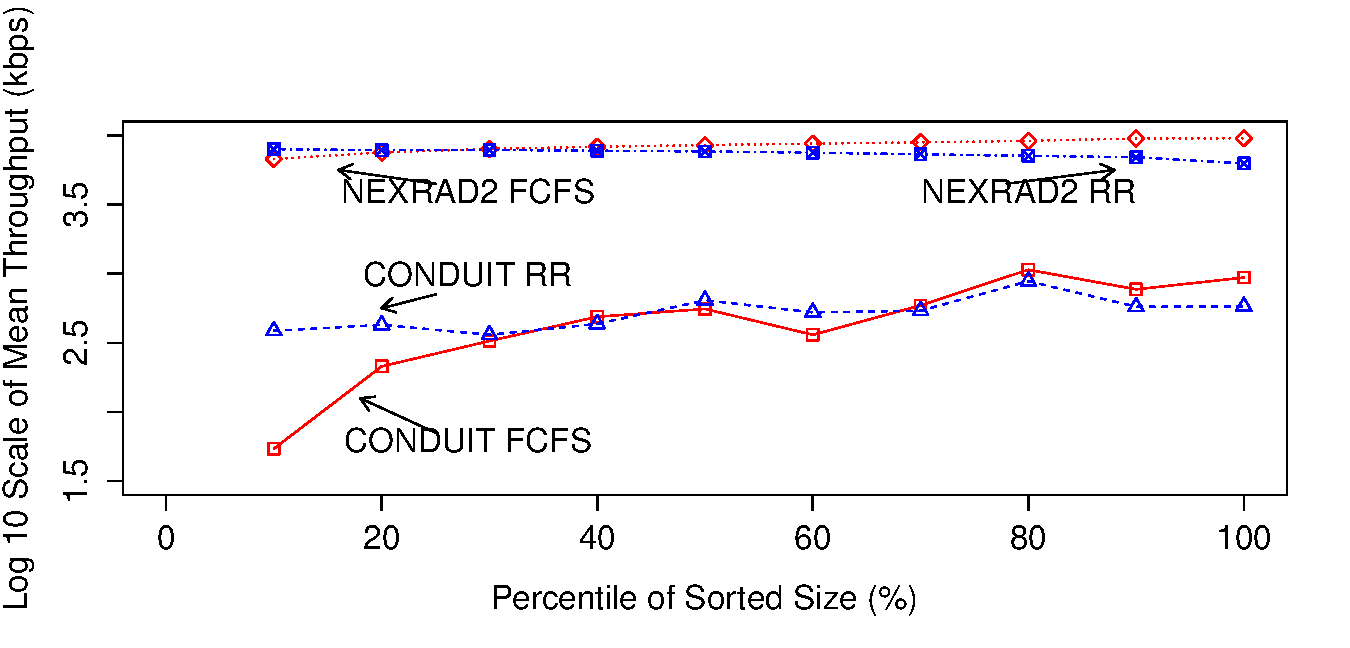
\includegraphics[width=0.5\textwidth]{figures/FCFS-vs-RR.pdf}
\caption{A comparison of per-bin mean multicast throughput values where each bin has 10\% of the files sorted by size}
\label{fig:FCFS-vs-RR}
\end{figure}

The utilization levels in Tables ~\ref{tab:RR-rate-buffer} and \ref{tab:FCSF-rate-buffer} are low, but as explained in Section~\ref{sec:LDM7}, packet scheduling
can be configured to operate in work-conserving mode, which means
that if the queue serving packets for a provisioned path is empty, the scheduler
will serve best-effort IP packets. The L2 path service is offered
on the same infrastructure as best-effort IP service in university campuses
and RENs. Therefore, network resources are not wasted during silence periods in the file-streams.

Finally, to gain a further understanding of FCFS and RR modes, we studied mean multicast throughput as a function of file size by dividing the size range
into 10 bins such that all bins had an equal number
of files. The per-bin mean multicast throughput values
for two feedtypes, CONDUIT and NEXRAD2, are plotted against size
percentile in Fig.~\ref{fig:FCFS-vs-RR}. As expected, smaller files fare better
in the RR mode, while larger files fare better in the FCFS mode
as can be seen in Fig.~\ref{fig:FCFS-vs-RR}. 

\subsection{Application of EWMA method for multiple days}
\label{sec:EWMA-results}
The EWMA scheme described in Section~\ref{sec:EWMA} is applied
to the week-long data for the CONDUIT feedtype when served using the RR mode. But before presenting the results computed using the actual rate
and buffer size set with the EWMA scheme,
Table~\ref{tbl:ideal-week} shows the ideal rate and buffer
size that should have been used each day. These numbers
are computed using the methods described in Sections~\ref{sec:buffer} and \ref{sec:rate-RR}.
\begin{table}[ht]
\caption{Ideal RR rate and buffer size computed with each day's data (post-facto); $\mathbb{G}=10$ kbps; $\beta=5\%$}
\centering
\begin{tabular}{| c | p{0.4in} | p{0.3in} | c | c| c |} \hline
Date & Rate (Mbps) & Buffer size (MiB) & Util. (\%) &  $\Theta$ (kbps) & $\eta_k$ (\%)\\ \hline
June 2 & 36 &248 & 12.4 & 535.2 &4.8 \\ \hline
June 3 & 30 & 362 & 14.3 &270.0 &4.8 \\ \hline
June 4 & 30&269 &15.0 & 424.7 & 4.9 \\ \hline
June 5 &30 & 249 &15.8 &695.5 &4.6 \\ \hline
June 6 &24 & 244 &18.6 &360.3 &4.6 \\ \hline
June 7 & 30 & 290 & 15.0 &514.1 & 4.8 \\ \hline
June 8 & 26 & 244& 16.8 &382.4 & 4.9 \\ \hline
\end{tabular}

\label{tbl:ideal-week}
\end{table}
In all rows of Table~\ref{tbl:ideal-week}, the RR throughput-violation rate
$\eta_k$ is smaller than the threshold $\beta$ value of 5\%.
The ideal rates computed for each day varies as the CONDUIT
model data is not exactly the same from day-to-day. Also, we see
a variation in the ideal buffer size required at the sending host
to achieve 0 loss. The utilization and mean multicast throughput values shown
in Table~\ref{tbl:ideal-week} are computed using the methods
described in Section~\ref{sec:output} but with the ideal rate and buffer
size settings, not the actual rate and buffer size settings.

Next, we present results from the application of the EWMA scheme
of Section~\ref{sec:EWMA}.
Two values of $W$ in \eqref{eqn:EWMA} are used to generate numerical
results.
Table~\ref{tbl:yesterday} shows results when $W=0$ and Table~\ref{tbl:W7} shows results
when $W=7$. With $W=0$, the ideal rate computed in the $k^{th}$ holding
interval is used directly in the $(k+1)^{th}$ holding interval.
With $W=7$, the ideal rate computed is given a weight of 0.125, while the running average rate is given a weight of 0.875.
\begin{table}
\caption{System performance with rate and buffer size computed using EWMA with $W=0$}
\centering
\begin{tabular}{| c | p{0.4in} | p{0.3in} | p{0.3in} | p{0.3in}| p{0.3in} |p{0.3in}|} \hline
Date & Rate (Mbps) & Buffer size (MiB) & Util. (\%) &  $\Theta$ (kbps) & $\eta_k$ (\%) & $\delta_k$ (\%)\\ \hline
June 3 & 36 & 248 & 12.0 &397.2 &3.2 &0.034\\ \hline
June 4 & 30 &362 &15.0 & 424.7 & 4.9&0 \\ \hline
June 5 &30 &362 &15.8 &695.5 &4.6&0 \\ \hline
June 6 &30 & 362 &14.9 &591 &3.4&0 \\ \hline
June 7 & 24 & 362 & 18.8 &309 & 7.2 &0.037\\ \hline
June 8 & 30 & 362& 14.6 &536 & 3.9 &0\\ \hline
\end{tabular}
\label{tbl:yesterday}
\end{table}
\vspace{-0.1in}
\begin{table}[!ht]
\centering
\caption{System performance with rate and buffer size computed using EWMA with $W=7$}
\begin{tabular}{| c | p{0.4in} | p{0.3in} | p{0.3in} | p{0.3in}| p{0.3in} |p{0.3in}|} \hline
Date & Rate (Mbps) & Buffer size (MiB) & Util. (\%) &  $\Theta$ (kbps) & $\eta_k$ (\%) & $\delta_k$ (\%)\\ \hline
June 3 & 36 & 248 & 12.0 &397.2 &3.2 &0.034 \\ \hline
June 4 & 35.3&362 &12.7 & 598.7 & 4.3&0 \\ \hline
June 5 &34.6 & 362 &13.7 &952.2 &3.7 &0\\ \hline
June 6 &34 & 362 &13.1 &780 &2.6&0 \\ \hline
June 7 & 32.8 & 362 & 13.8 &626 & 4.1&0 \\ \hline
June 8 & 32.4 & 362& 13.5 &643 & 3.8&0 \\ \hline
\end{tabular}

\label{tbl:W7}
\end{table}

In Table~\ref{tbl:yesterday}, we see that the rate used for June 3, which is 36 Mbps, is the  ideal rate computed for June 2, as seen in Table~\ref{tbl:ideal-week}. A similar pattern is observed in subsequent rows when comparing rates of Tables~\ref{tbl:ideal-week} and \ref{tbl:yesterday}. The
buffer size in Table~\ref{tbl:yesterday} increases to 362 MiB, but
stays at that level, which means the traffic on subsequent days did
not cause a larger backlog than it did on June 4. The only day
in which the EWMA scheme with $W=0$ violated the RR throughput-violation
rate is on June 7, when $\eta_k$ reached 7.2\%, exceeding the $\beta$
threshold of 5\%. Correspondingly, there were dropped files, with the dropped-file rate $\delta_k$ reaching 0.037\%. For
all days, the actual rates used, as indicated in Table~\ref{tbl:yesterday}
are higher or equal to the ideal rates presented in
Table~\ref{tbl:ideal-week}, except for June 7, when the ideal rate
was 30 Mbps, but the actual rate used was only 24 Mbps.

The second $W$ setting of 7 worked well. On June 7, as seen in Table~\ref{tbl:W7}, the actual rate used was 32.8 Mbps, while
the ideal rate as seen in Table~\ref{tbl:ideal-week} was only 30 Mbps.
Table~\ref{tbl:W7} shows that there were dropped files ($\delta_k = 0.034\%$) on June 3, which being the first day, did not have the benefits of rate averaging and buffer maximization.


The results presented here are examples of how the EWMA scheme works.
In a practical deployment, the particular $W$ value will need to be
selected for each feedtype, as the day-to-day variation in traffic
depends on the feedtype.

\section{Related work}
A MultiPath MultiCast (MPMC) algorithm to distribute a file to multiple receivers, with segments of files being transmitted
on multiple paths, is proposed and evaluated on OpenFlow networks \cite{6630542}.
The problem statement of this work is different from ours, i.e., unlike in our work, path rate computation is not an objective in the MPMC algorithm development.

A paper on Layer-2 multicast in OpenFlow networks for multimedia distribution
(VLC streaming) \cite{6799481} compares the ease of using of OpenFlow-enabled
Layer-2 multicasting with IP multicasting and application-layer multicasting.
The path setup phase in OpenFlow-controlled L2 multicasting negates the need for distributed multicast routing protocols, which has proven to be challenging but necessary for IP multicasting. A method for dynamic path adjustment of OpenFlow-controlled multicast trees is presented by Ge et al. \cite{6681003}.

An interesting use of OpenFlow control to isolate elephant flows, which are termed ``significant flows'' and hence worthy of per-flow setup actions, was proposed \cite{Curtis:2011:DSF:2018436.2018466}. It is related to our work because it uses OpenFlow for path setup for particular flows, but the issue of rate computation is not addressed.
The use of QoS controls in OpenFlow networks is explored in a testbed \cite{6385057}, and proposed for video streaming \cite{6116083}.

Finally seminal work on how to compute rate for a virtual circuit
for a given traffic model was done by Guerin et al. \cite{103545}.
This work was applied for audio and video streams for which the modeling
assumptions held. These assumptions do not hold for our file-stream traffic. 

\section{Summary and conclusions}
This work identified an exciting new problem
of rate determination for L2 multipoint virtual topologies
to serve variable-rate file streams to multiple receivers. Prior work
on rate computation methods were designed for audio/video
streams, not file streams. The problem is based on the need
for scalability in a real deployment as data volumes and
number of receivers have grown. Our solution was based, not
on models, but on actual traffic characteristics. These
characteristics, such as right-skewed file size and file
inter-arrival times, and variability from day-to-day,
are likely to hold for other types of file-streams. 
Our solution, based on a empirical method and an exponential weighted moving average scheme, was designed
to have broad applicability, not customized for the IDD feedypes.
Evaluation of our method with real traffic (from five IDD feedtypes) showed that
while throughput constraints can be met by selecting a suitably high
rate, utilization varies based on the burstiness of each file-stream.
However, if rate-guaranteed L2 services are offered
on the same network as best-effort IP services, and packet schedulers
are configured to operate in work-conserving mode, the utilization levels
of the L2 multipoint topologies are not of significant concern.


%\chapter{Local Data Manager Performance Measurement}
\label{sec:ldm}
\section{Introduction}
The main goals of this work are to develop
tools and techniques to quantify LDM-6 performance
across WAN-paths. Specifically, various input parameters
were controlled and LDM-6 throughput and resource requirements
were measured. The objective is to have the shell scripts
and log parsers in place for the LDM-6 vs. LDM-7 comparison.


\section{Evaluation of LDM-6 across WANs experiments}

Two testbeds were used to characterize LDM-6 performance and resource requirements: DYNES and GENI.

For the DYNES experiments, the following sites were used: UVA, Rutgers, UWisc, IU, MAX, and I2 Labs. Each DYNES site has a high-performance host called Fast Data Transfer (FDT) host
for running applications, a perfSONAR
host, an Inter-Domain Controller (IDC) that runs OSCARS and optionally OESS, and an OpenFlow (or CLI
controlled) switch. The high-performance hosts have two 10G NICs connected to the DYNES switch,
and 1G NICs connected to the campus networks. The latter were used in our LDM-6 testing. The reason for choosing these 1G NICs was to measure LDM-6 performance
across IP-routed paths. For the DYNES experiments, the LDM6 sender was run at UVA FDT, and the receivers
were located at Rutgers, UWisc, IU, MAX, and I2Labs FDT servers. LDM-6 uses
unicast TCP connections.  Specifically the DYNES FDT hosts were configured to use HTCP.

For the tests on GENI, the following ExoGENI racks were used: UFL (sender), and TAMU, WSU, UMass, and OSF
(for the receivers). Since GENI slices include L2 VLANs between hosts, we executed LDM6 over Circuit TCP (CTCP),
which is our implementation of a null congestion control module that plugs into Linux kernel. CTCP has three parameters: Bandwidth-Delay Product (BDP), which was computed and set to 150 packets, rate was set to 20 Mbps (suitable for the NGRID taffic) and scale was set to 1.2. The scale factor is multiplied by the BDP value to set the unchanging congestion window. The Linux tc TBF parameters were set as follows: rate: 80 Mbps, burst: 50 KB, and limit: 1.4 Mbits.

Steve Emmerson implemented a software tool called \texttt{pqinsert} to read the NGRID metadata, and populate a memory-mapped product queue with dummy-bits filled data-products.  The metadata needed to be
sorted according to creation time before it could be read by \texttt{pqinsert}. 

The measure of throughput was an aggregate value
computed for groups of data-products, each of which had a total size of 200 MB. A Python program was coded
to parse LDM-6 logs to extract creation time, arrival time, and product size for each product,
and then compute the aggregate throughput for each 200-MB sized group of data-products.

Next, to obtain resource requirements, a monitoring shell script was written to start a \texttt{ps-script} and \texttt{tcpdump}
for collecting CPU usage, and bandwidth usage measurements, respectively. The \texttt{ps-script} ran the Linux \texttt{ps} utility with appropriate arguments to collect CPU-usage every min. This monitoring shell-script
was started before the LDM-6 processes.  Upon completion of the 7-hour run, a Python program was run
to parse \texttt{ps-script} output and find the per-min CPU usage. The \texttt{tshark} program is used to
parse the \texttt{pcap} file collected by \texttt{tcpdump} to determine bandwidth usage by each
LDM-6 TCP flow.  A Python program is currently under development to parse the \texttt{tshark} output
to visualize bandwidth usage as a function of time.

Input parameters that influence LDM-6 throughput and resource requirements are (i) number of receivers, (ii) rate (ii) packet loss, and (iv) sender and receiver hosts (RTT and differences in host characteristics affect results).
For the DYNES and GENI tests, metadata for the first 7 hours of the 24-hour collected NGRID metadata was used. 

\section{Results}

\subsection{LDM6 per-file throughput and aggregate size throughput}

Fig.~\ref{fig:single-file-throughput} shows that single products can enjoy close to 1Gbps throughput,
but most products experience about 10 Mbps.  The RTT on this path is 9.3 ms.  Given the impact
of file arrival times and file sizes, the aggregate throughput is a better measure than single-file throughput.
Fig.~\ref{fig:DYNES-throughput} shows the dependence of aggregate throughput on RTT. The RTT values from
UVA FDT host to the FDT hosts at I2-Labs, IU, MAX, Rutgers and U.Wisc. are 38.4, 36.8, 4.4, 9.3 and 47.4ms,
respectively. As UVA-MAX path has the smallest RTT, this connection enjoys the highest throughput. 
\begin{figure*}
\centering
\begin{subfigure}[b]{0.47\textwidth}
\centering
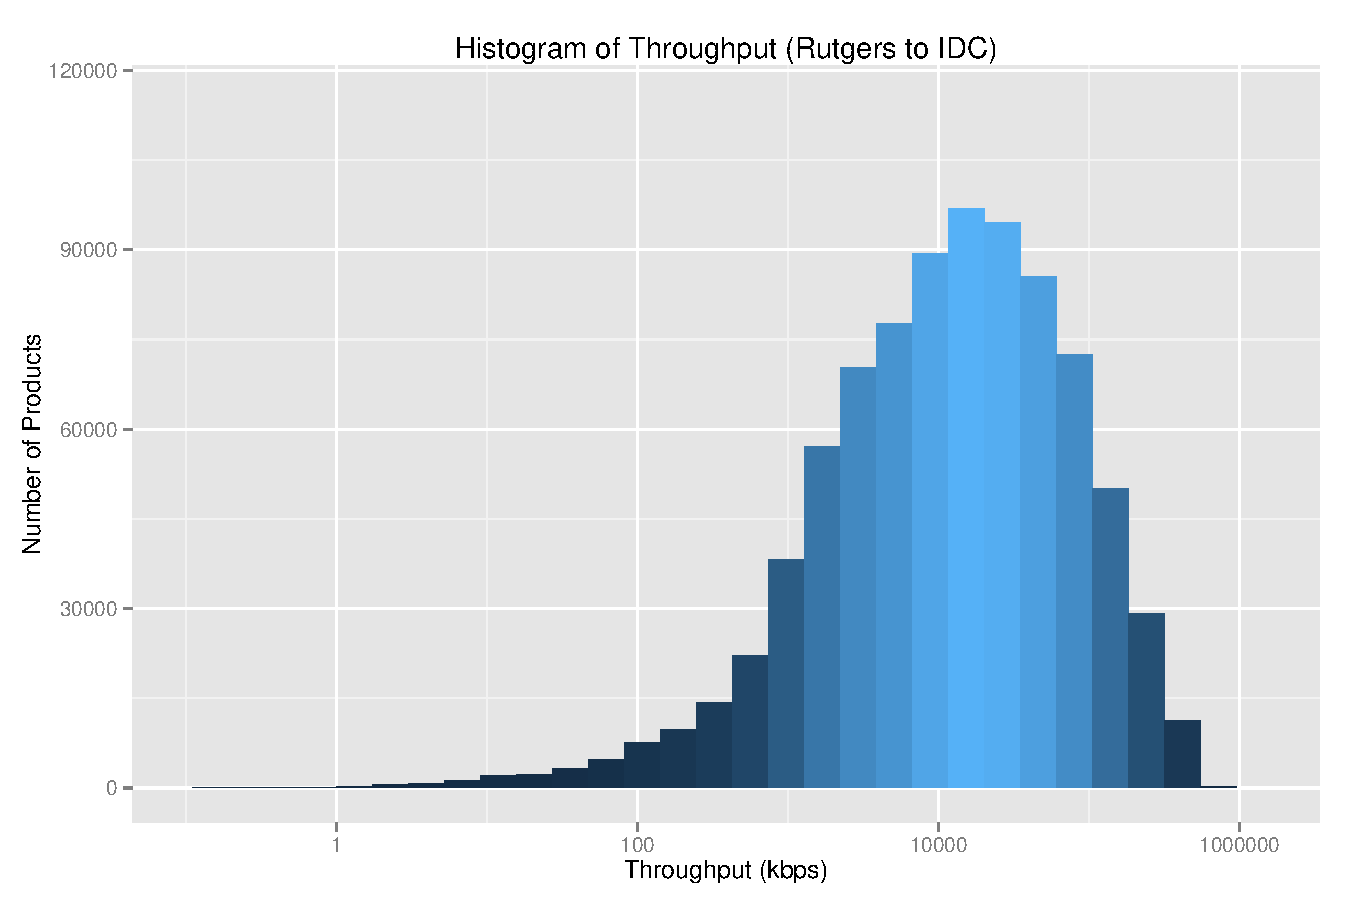
\includegraphics[width=0.9\textwidth]{figures/1-day-1-rcv-single-product-throughput.pdf}
\caption{Histogram of single file throughput measurements for LDM6 transfer from Rutgers FDT to UVA IDC}
\label{fig:single-file-throughput}
\end{subfigure}
\begin{subfigure}[b]{0.47\textwidth}
\centering
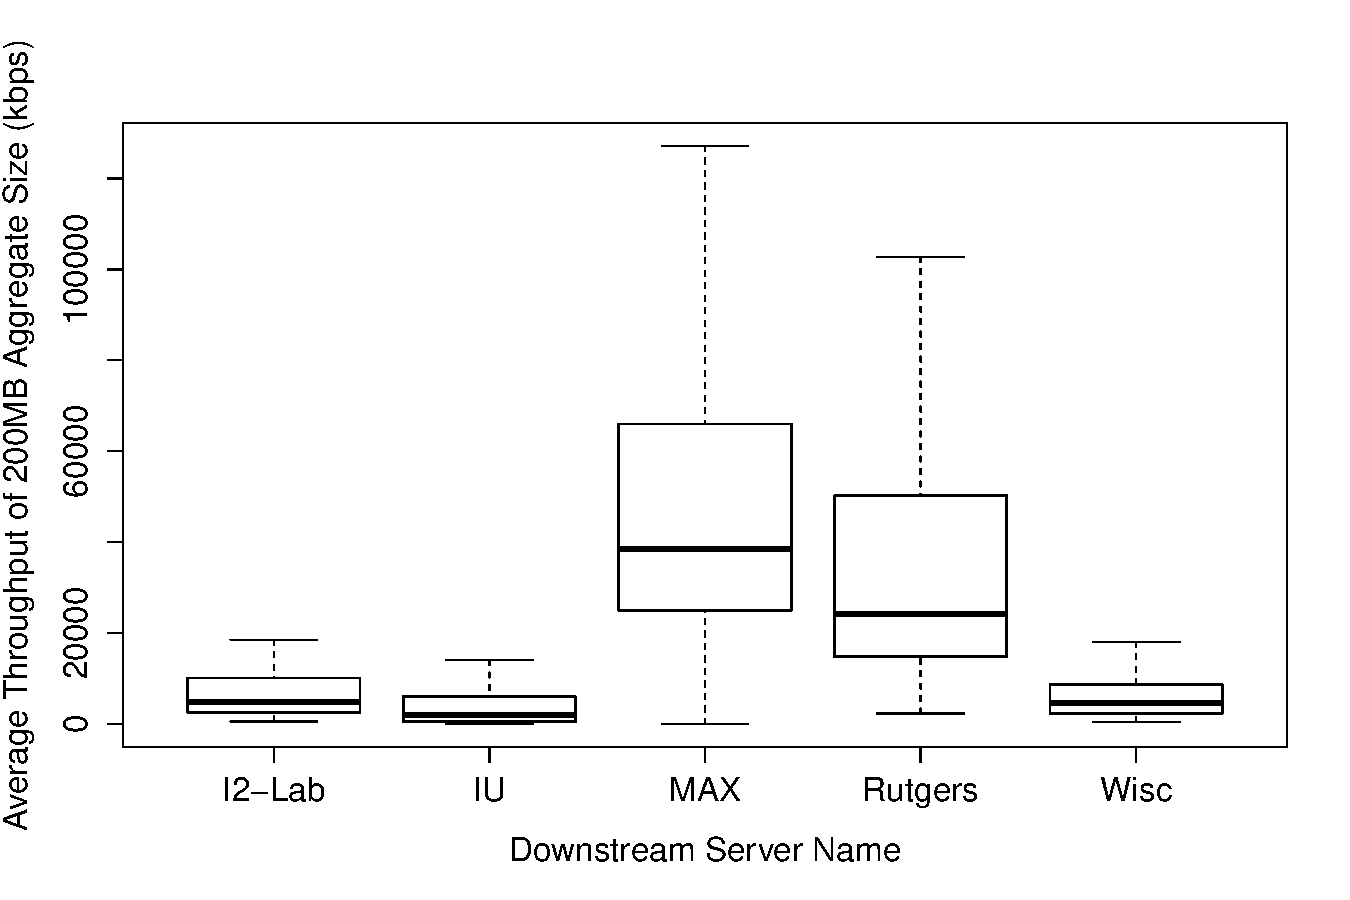
\includegraphics[width=0.9\textwidth]{figures/DYNESThroughput_IP_Path.pdf}
\caption{Sender at UVA; Receivers at the five listed sites}
\label{fig:DYNES-throughput}
\end{subfigure}
\caption{LDM-6 throughput in DYNES experiments}
\label{fig:marking-rate-effects}
\end{figure*}

\begin{figure*}
\centering
\begin{subfigure}[b]{0.47\textwidth}
\centering
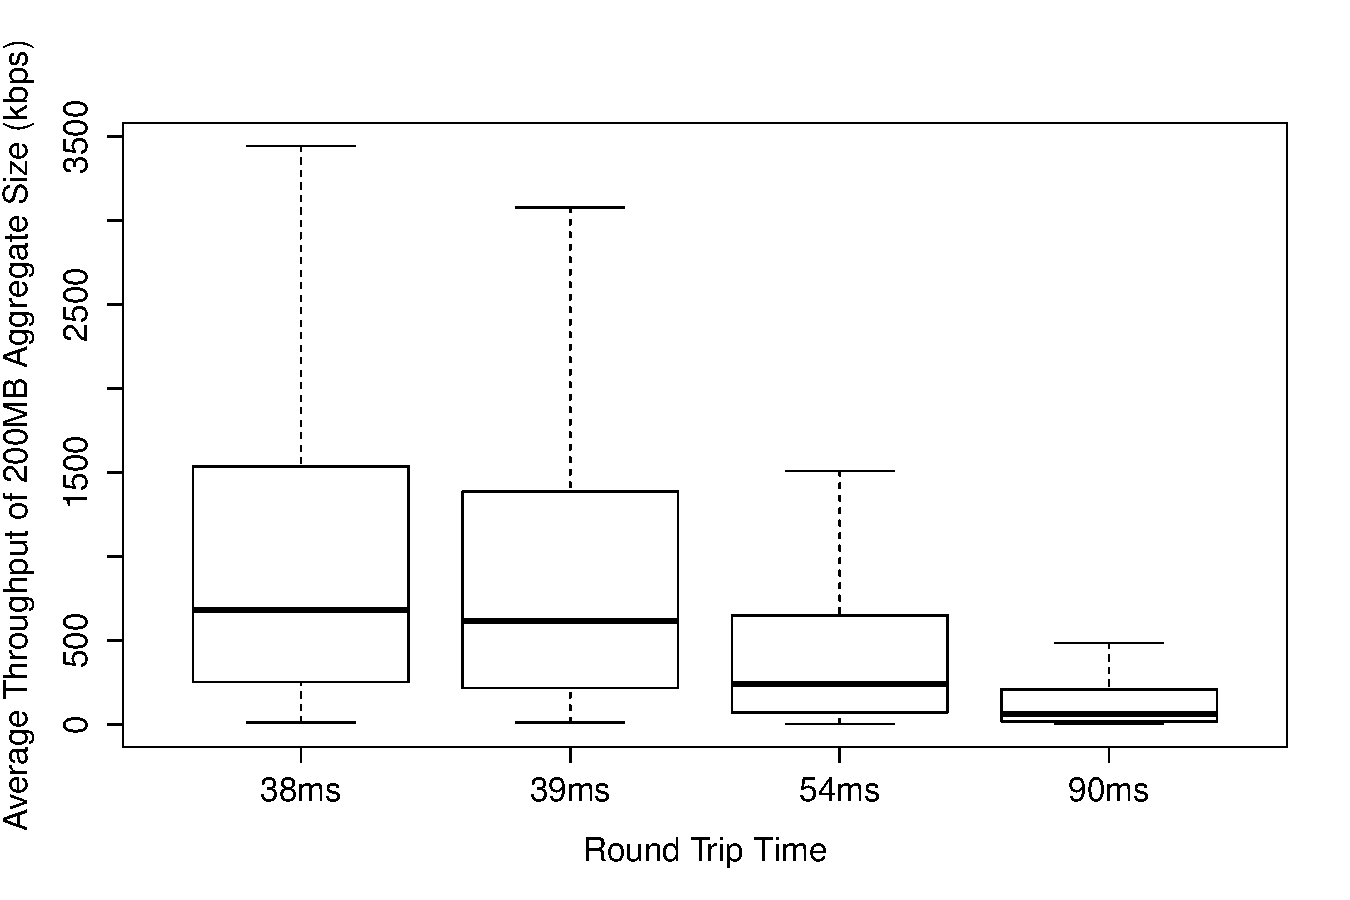
\includegraphics[width=0.9\textwidth]{figures/GENI_Throughput_BoxPlots_RTT.pdf}
\caption{Boxplots comparing aggregate throughput on paths to 4 receivers}
\label{fig:GENI-4-rcv-boxplots}
\end{subfigure}
\begin{subfigure}[b]{0.47\textwidth}
\centering
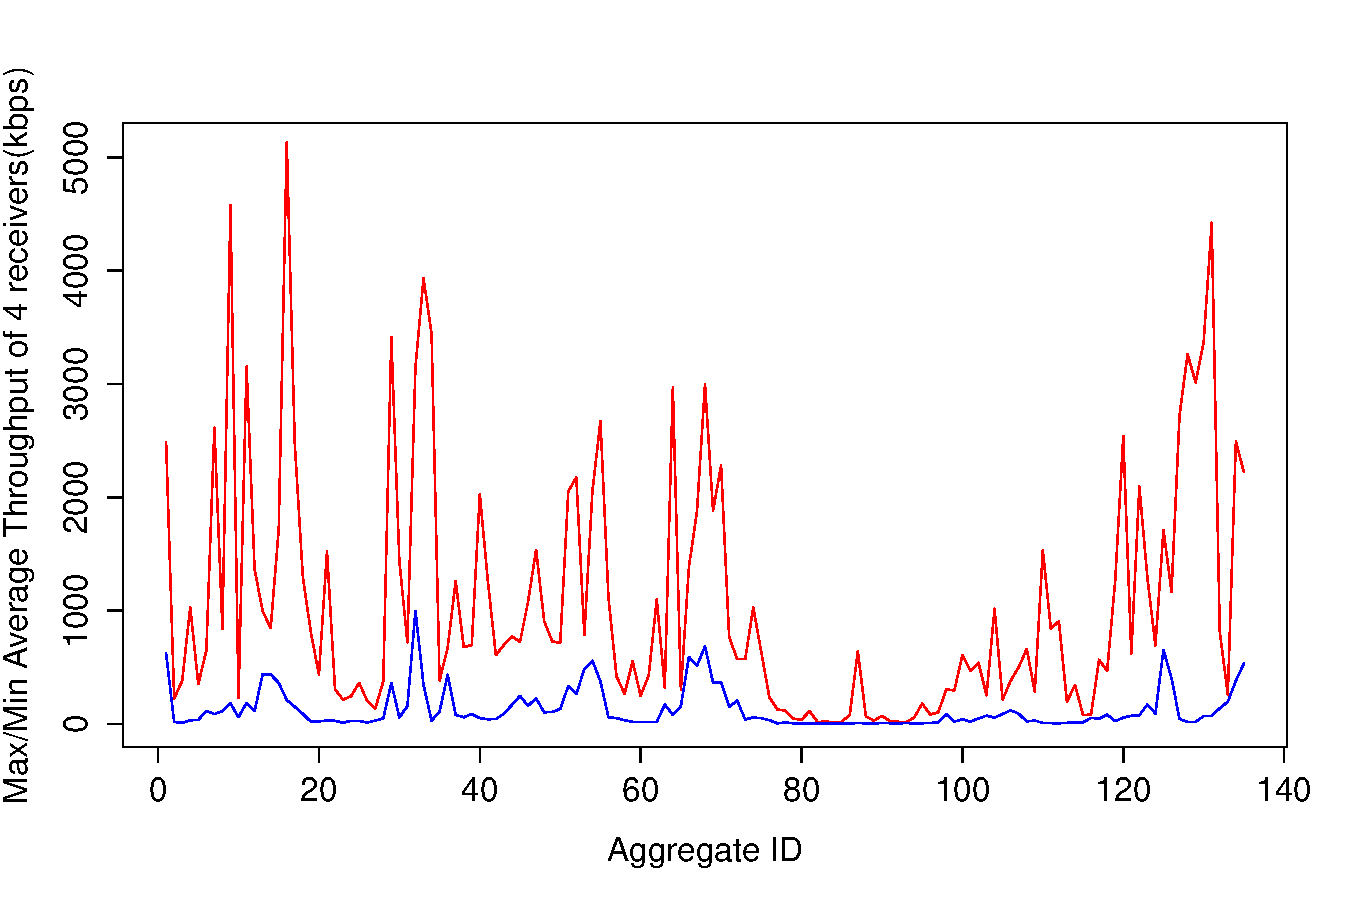
\includegraphics[width=0.9\textwidth]{figures/GENI_Throughput_vs_AggregateID.pdf}
\caption{Min and Max aggregate throughput among the four paths}
\label{fig:min-max-throughput-GENI-LDM6}
\end{subfigure}
\caption{LDM-6 throughput in GENI experiments}
\label{fig:GENI-LDM6}
\end{figure*}

Fig.~\ref{fig:GENI-LDM6} shows the the aggregate throughput measurements obtained in the GENI
experiments. Fig. ~\ref{fig:GENI-4-rcv-boxplots} compares the aggregate throughput on the paths
to 4 receivers. The RTTs on the paths from  UFL (sender) to the receivers at UMass, WSU, TAMU, and OSF, were 38, 39, 54 and 90 ms, respectively. Since CTCP was used in these GENI experiments, we did not expect a dependency on RTT.
However, the mean data product size is 65 KB for NGRID, and with the 20 Mbps sending/path rate, the mean transmission delay for products in each aggregate is only 26 ms. Thus, the RTT lowers the average throughput significantly.

Fig.~\ref{fig:min-max-throughput-GENI-LDM6} shows the minimum and maximum throughput for each aggregate
from the measurements obtained for the four paths. These results show that there is significant dependence of
the aggregate throughput on the inter-arrival times and sizes for files within each aggregate.

With respect to resource requirements, we found that the CPU usage at the sender host was 0.4\% 
when there were 4 receivers, and the usage increased linearly with the number of receivers. We are currently generating the bandwidth usage results.

\subsection{LDM CPU usage}

\subsection{LDM6 throughput for constant aggregate size, from UCAR to UVA}

\subsection{LDM Measurement of Packet loss}

\section{TCP restart measurement}

\section{Topology changing of IDD feedtypes}
\subsection{Experimental setup}
Steve setup a cron job at \emph{uni16.unidata.ucar.edu} which is one of the LDM upstream servers, the cron job executes a uldbsend command every hours to send uldbutil report to \emph{fdt-uva.dynes.virginia.edu}.

At UVA FDT site, two configuration file, ldmd.conf and pqact.conf need to be set, the detail setup is in \emph{https://github.com/XiangJi/CC-NIE-LDM/tree/master/uldbutil}. These configurations will make sure UVA FDT hosts can receive any data from UCAR servers and save the data as file locally. 

\subsection{uldbutil report}
uldbutil (Upstream LDM database utility) report provides the subscribers information for that hosts. Sample entry like: $12948 6 feeder awipsops.nsstc.uah.edu$ $20160106205353.878 TS_ENDT (CONDUIT,  .*) primary$ shows that the subscription instance 12948 whose hostname is \emph{awipsops.nsstc.uah.edu} using LDM 6 requested CONDUIT feedtype data from 20160106205353.878.

\subsection{Scripts for tracking the receivers changing for Top 5 feedtypes}
A Python script is written for counting how many receivers are requesting Top 5 feedtypes from the uldbutil report and writing the results into a csv file. This program will be executed every hour for tracking how do the subscribers change.

\section{Results}
\begin{figure*}[htb!]
\centering 
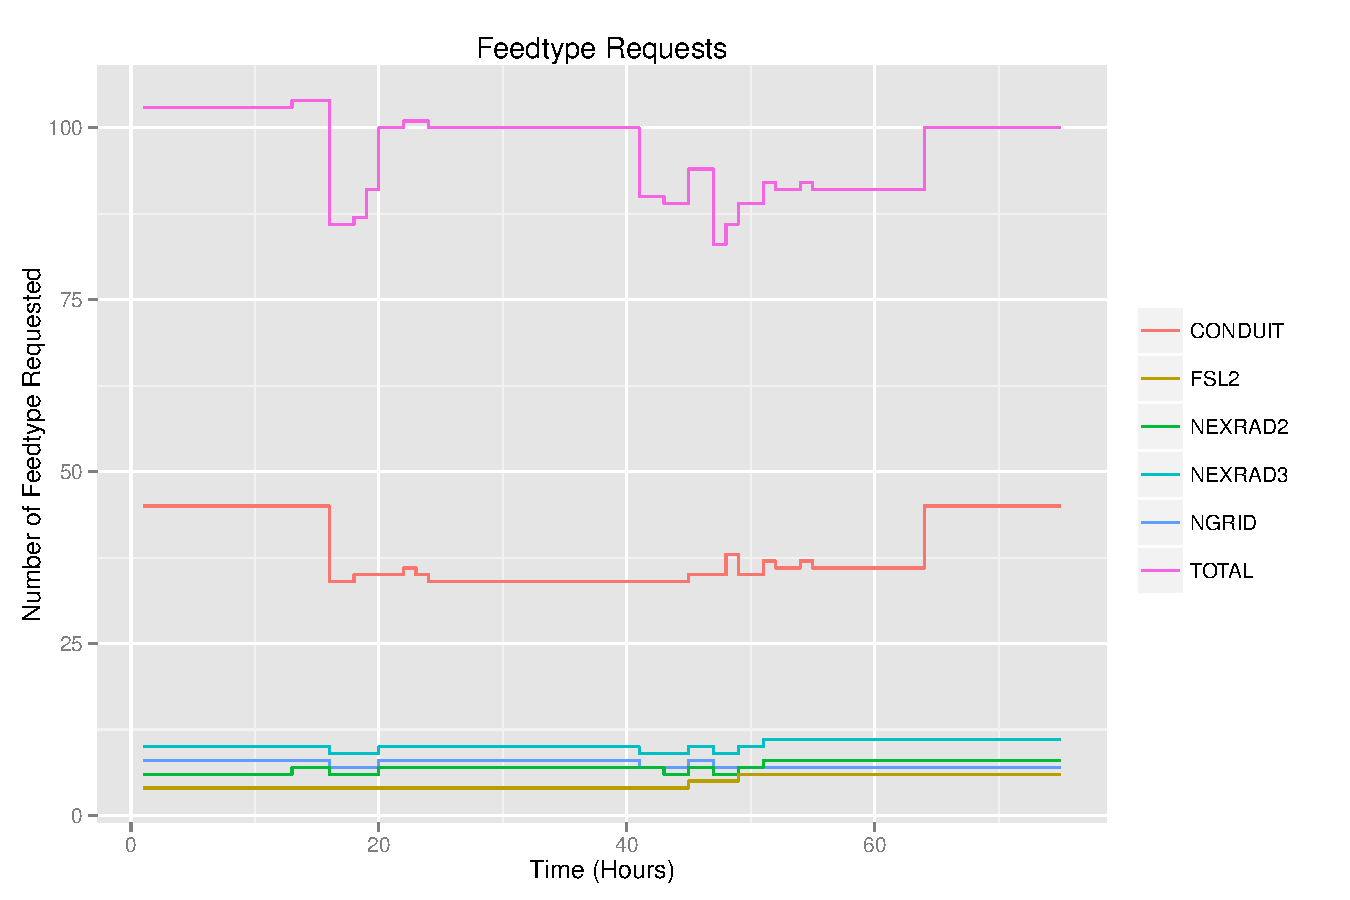
\includegraphics[width=0.96\textwidth]{figures/uldb_track.pdf}
\caption{Tracking subscibers for Top 5 feedtypes, number of subscibers for each feedtype}
\label{fig:uldb}
\end{figure*}

Fig.~\ref{fig:uldb} shows that how do the subscribers number change in 3 days for Top 5 feedtypes. It indicates that CONDUIT is the major feedtype the weather data research institutions are subscribing. By using the uldbutil report, we can record which receiver is requesting which feedtypes data. This report can inform the LDM control to use OESS to change the OpenFlow path with corresponding endpoints and bandwidth need to be reserved.  



\section{Conclusions}
The monitoring tools have been developed, shell scripts have been coded, and Python and R programs have been implemented to execute a systematic set of experiments on GENI and LDM to obtain measurements for throughput and resource
consumption. Preliminary results have been obtained on both testbeds. Rutgers (Slezak and Decker)
are working with us on LDM6 experiments, and U. Wisc (Robaidek) is working with us on LDM7 testing and evaluation. Rutgers will also test LDM7.

\chapter{A Multi-Domain SDN for Dynamic Layer-2 Path Service}
\label{sec:DYNES}

The term ``domain'' is used to represent a network that is owned and operated by
a single organization, e.g., University of Virginia's domain, AT\&T's domain.
To establish and release layer-2 VLANs that traverse multiple domains requires sophisticated
control-plane operations.

\section{Introduction}

Over the past decade, the high-performance research-and-education (R\&E) networking
community that supports scientific computing has invested in developing architectures,
protocols, and
software controllers to support rate-guaranteed
dynamic Layer-2 (L2) path services \cite{1541694,4444698,4374315,1497551,4146687,OSCARS,OESS,1742-6596-396-4-042065}.
Applications include
(i) large dataset transfers \cite{UVA-CTRQ2013},
(ii) reliable multicast of file stream \cite{ji2015file},
(iii) high-rate delay-sensitive interactive
applications such as remote visualization and remote
instrument control, and (iii) resource isolation in virtualized networks \cite{GENI}.

To support rate-guaranteed dynamic L2 path services,
two components are required. \emph{First},
switches/routers should have data-plane support for classifying packets into flows, policing flows on ingress ports to ensure that they do not exceed their rate allocations, and scheduling packets on egress ports according to their flow-rate allocations. \emph{Second}, control-plane support
is required for admission control to check whether sufficient bandwidth resources are available before accepting a path-setup request, provisioning the path prior to usage (which means setting label mappings in switches for data-plane packet forwarding), and releasing resources and label mappings upon completion of usage. The introduction of OpenFlow/SDN technologies reduces the barriers to deploying dynamic rate-guaranteed L2-path service since the required control-plane software can be implemented in an external SDN controller rather than in switches.

Considerable advances have been made in enabling dynamic L2-path service.
\emph{First}, control-plane protocols have been specified and are being standardized. These
include Inter-Domain Controller Protocol (IDCP) \cite{IDCP} and the
Open Grid Forum Network Service Interface Connection Services (NSI CS) version 2.0 \cite{NSI}. Both protocols support
inter-domain signaling for advance-reservation and provisioning of rate-guaranteed
dynamic L2 paths. \emph{Second}, Internet2 and ESnet, the two major US backbone Research-and-Education
Network (REN) providers, have
deployed SDN controllers and Layer-2 switches to
support dynamic L2 path service. These controllers
include Open Exchange Software Suite (OESS)\cite{OESS} and
On-Demand Secure Circuits and Advance Reservation System (OSCARS)\cite{OSCARS}. OESS is an intra-domain
SDN controller that controls switches via OpenFlow, while
OSCARS supports inter-domain service.

The \emph{contributions} of this work are that we leveraged an existing deployment
called Dynamic Network System (DYNES) \cite{1742-6596-396-4-042065}, in which small SDNs were deployed
in multiple university campuses and regional RENs, to test multi-domain dynamic L2 path service. This thesis
offers insights into the complex issues that we encountered in deploying OESS and OSCARS in multiple domains (organizations), and describes the problems we encountered while provisioning inter-domain dynamic L2 paths. These problems can be solved to continue growing this dynamic L2-path service. The work presented in this chapter was
published in ACM NDM 2015 \cite{tepsuporn2015multi}.

The \emph{novelty} of this work is that it reports on a multi-domain SDN service in
which an inter-SDN-controller protocol is used for cooperative dynamic L2-path reservation and provisioning. Prior papers on SDN, e.g., Google B4  \cite{Jain:2013:BEG:2486001.2486019} and Microsoft's SWAN \cite{Hong:2013:AHU:2486001.2486012} are single-domain deployments. The GENI stitching approach
\cite{GENI-stitching} uses a tree model
that is designed to support network researchers. Our objective is to create
a scalable solution for a broader range of use cases.
Previous work on DYNES \cite{1742-6596-396-4-042065} described the use of OSCARS, and data-plane experiments. Our work builds on this prior work and makes the new contributions listed above.

The \emph{impact} of this work can be far-reaching. Our dynamic L2 service deployment is comparable to the early ARPAnet deployment of IP-routed service in 1970, when there were fewer than 10 connected universities. Just as ARPAnet grew into today's Internet with its IP-routed (L3) service, our seed deployment of a multi-domain rate-guaranteed dynamic L2 path service reaching 8 campuses could grow into a global-scale service, offering an opportunity for new delay-sensitive applications that are not supported well on today's best-effort IP service.

Section~\ref{sec:control-plane} describes the control plane software OESS and OSCARS, the provisioning process of the integrated system.
Section~\ref{sec:mdsdn} describes our experience of equipment setup, OESS GUI for reserving an OpenFlow path, hosts configuration for path provisioning.
Section~\ref{sec:insights} describes the lessons we learned from the experiments, the scalability of the system, and the troubleshooting process.
Section~\ref{sec:mdvlan} describes my experiments from an inter-domain multi-point VLAN, basically the process of provisioning by AL2S OESS and data plane work. 



\section{Background}
\label{sec:control-plane}
This section describes the two control-plane software systems, OESS and OSCARS. OESS is an OpenFlow controller
that accepts user advance-reservation requests for L2 paths
(in which start time, rate, duration, and endpoints are specified), performs intra-domain path computation, and configures rules in the switches along the path for VLAN based
packet forwarding using OpenFlow. OSCARS performs similar functions, and additionally supports inter-domain path
reservations and provisioning. Also, it can communicate
with a variety of switches/routers including some that do not
implement OpenFlow. Both OSCARS and OESS offer users
a Web Browser User Interface (UI) and a programmatic Web Service Interface for applications. In this section, we briefly
review the functionality offered by these controllers.
OESS supports integration with OSCARS, specifically to support inter-domain circuits.

\subsection{On-Demand Secure Circuits and Advance Reservation System (OSCARS)}
We review the overall OSCARS architecture, describe how trust/peering relationships are established between neighbouring OSCARS, and how topology is discovered before presenting how OSCARS reserves resources and provisions and releases paths (which is its main role). We end with a short review of path computation, which is executed during resource reservation \cite{OSCARS}.

\paragraph{Software architecture}
The OSCARS software consists of 11 modules that have distinct functions such as authentication, authorization, path finding, messaging, hardware mediation, and process coordination. Today, OSCARS supports inter-domain L2 paths using both the Inter-Domain Controller Protocol (IDCP) \cite{IDCP} and Network Service Interface Connection Services (NSI CS) version 2.0 \cite{NSI} protocols. The authorization (i.e., policy enforcement) of guaranteed bandwidth reservation requests are domain specific and can be enforced using the policy path computation modules within the OSCARS v0.6 Path Computation Engine (PCE) framework.

\paragraph{Trust/peering relationships}
The current trust model for
inter-domain dynamic paths is based on transitive peer-to-peer authentication and authorization. This work-flow mimics the telecommunication industry model; neither require downstream providers to know anything about the originating caller.

\paragraph{Topology discovery}
Each domain is responsible for discovering and pushing its topology to the perfSONAR Topology Service (pS-TS). The distributed pS-TS maintains
global topology information, and OSCARS servers can pull
the latest information from pS-TS as needed in real-time.
Topology information must be formatted in either the Open
Grid Forum Network Markup Language (NML) \cite{van2013network} or the NM-Control Plane \cite{IDCP} schemas to support the NSI CS v2.0
and the IDCP protocols, respectively.

\paragraph{Inter-domain L2 path reservation, provisioning, and
release}
When the OSCARS server in a domain receives an inter-domain VC reservation request, it reserves resources within its
own domain and sends a \texttt{createReservation} message
with endpoints, rate, start time (advance-reservation support)
and duration, to the OSCARS in the next domain, which is
selected based on the computed path. The procedure is executed in a daisy-chain fashion, as shown in Fig.~\ref{fig:daisychain},
until the OSCARS of the last domain on
the end-to-end path is reached. If successful, \texttt{Confirmation}
events are sent from one domain’s OSCARS server to the next
in the reverse direction. Provisioning of the VC occurs either
automatically or upon receiving a \texttt{createPath} message
from the user just before the reservation start-time. This procedure also uses a daisy-chain of signaling messages between
OSCARS servers. Each OSCARS server communicates with
the switches in its domain to provision the VC across the
domain. Finally, when the reservation end-time is reached a
\texttt{teardownPath} message is sent in daisy-chained mode to
release the VC.

The current trust model for inter-domain dynamic paths is based on transitive peer-to-peer authentication and authorization. This work-flow mimics the telecommunication industry model; neither require downstream providers to know anything about the originating caller.
\begin{figure}
\centering
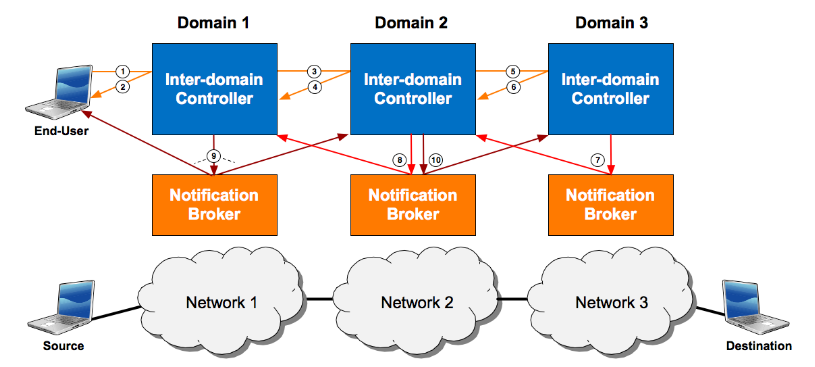
\includegraphics[width=0.6\textwidth]{figures/daisychain.png}
\caption{Daisy-chain model used by OSCARS for inter-domain circuit reservation, provisioning, and release}
\label{fig:daisychain}
\end{figure}

\paragraph{Path computation} In OSCARS v0.6, path computation
executed using ``atomic" Path Computation Engine (PCE) modules that can be
arbitrarily linked together. Each PCE module typically addresses a
specific constraint and prunes the graph accordingly. For example, a bandwidth PCE would discard all links that do not
have sufficient bandwidth, and a policy PCE would remove
all resources that the requester is not authorized to use.
While the PCE methods surveyed by Paolucci et al. \cite{6422287} are
for immediate-request paths, the OSCARS PCE supports
advance-reservation paths.


\subsection{Open Exchange Software Suite (OESS)}
\label{sec:OESS}

The Open Exchange Software Suite (OESS) is an OpenFlow
controller used to configure and control dynamic L2 paths
across a network of OpenFlow-enabled switches. OESS provides sub-second circuit provisioning, automatic circuit failover, per-interface permissions, and automatic per-VLAN
statistics.

\paragraph{OpenFlow path provisioning}
When a user wishes to provision an L2 path in OESS, the user must first select the endpoints (at least 2), rate, start time, duration, VLAN IDs, and optionally specify a path (with possibly a backup path) that connects all endpoints. In this context, endpoints are OpenFlow switch ports. For example, in Fig.~\ref{fig:oscarsoess}, consider the two numbered ports: port 19 of the DYNES switch in the University 1 network, and port 20 of the DYNES switch in the University 2 network. These two ports are the endpoints specified in a request for an end-to-end L2 path between the FDT hosts at University 1 and University 2.

Once the user has specified all the parameters in the request, the OESS UI sends the request to a Forwarding Controller. The Forwarding
Controller then calculates the \texttt{OFFlowMods}, which is a specification of the OpenFlow rules required to provision the path.
Each switch will receive at least 2 \texttt{OFFlowMods} (in cases of
multiPoint VLANs, there can be more than 2 \texttt{OFFlowMods}).
Each \texttt{OFFlowMod} is broken up into a \texttt{Match} and an \texttt{Action}.
The OpenFlow Match is applied to all packet headers, and
if a packet matches all of the fields in the OpenFlow \texttt{Match},
all of the OpenFlow \texttt{Actions} for the \texttt{OFFlowMod} are then
applied to the packet.

OESS has implemented a specific set
of OpenFlow \texttt{Matches} and \texttt{Actions}. All OESS \texttt{OFFlowMods}
for a VC consist of a \texttt{Match} that contains the input port
(\texttt{IN\_PORT}) and input VLAN ID (\texttt{DL\_VLAN}) fields. The
\texttt{Actions} consist of \texttt{SET\_VLAN\_ID} and OUTPUT (to a port)
actions. In some cases, the \texttt{STRIP\_VLAN} action is also used
(for untagged circuits). OESS uses NOX \cite{gude2008nox} to send \texttt{OFFlowMods} to the OpenFlow switches as shown in Fig.~\ref{fig:ControlPlane}.

In a network with QoS support, the controller would issue commands to configure filters, policing and scheduling in the OpenFlow switches so that flows do not violate the rates specified during path reservation. OpenFlow 1.3.0 supports QoS features, but the OESS implementation used in this study supported only OpenFlow 1.0 because Internet2 AL2S, for which OESS was initially designed, had only OpenFlow 1.0 switches when this study was carried out.

\paragraph{Topology discovery}
OESS learns the topology for its domain,
through a protocol similar to Link Layer Discovery Protocol (LLDP), called OpenFlow Discovery Protocol (OFDP) \cite{OFDP}.
OFDP functions by having the controller generate a packet
and send the packet out on every interface of an OpenFlow
switch using the \texttt{OFPacketOut} mechanism. The packet that
is sent out on each interface is tagged with the \texttt{DataPathID}
(a unique identifier for each OpenFlow Switch that is usually
based on a management MAC address) and number of the
interface on which the packet was sent. A rule is configured on
all switches to ``punt'' these topology-discovery packets to the
controller through an \texttt{OFPacketIn} event. The \texttt{OFPacketIn}
event sends the packet that arrived at the switch along with the
port and \texttt{DataPathID} of the switch that received the packet.
When this procedure occurs in both directions of an inter-switch link, an adjacency
is detected and OESS creates a link between the two devices on
the specified ports. OESS can also detects link failures and
node insertions, allowing for the OESS to automatically move
thousands of VLAN VCs with minimal human intervention.

% \paragraph{OESS software architecture}
% Fig.~\ref{fig:ControlPlane} shows the software architecture of OESS. OESS provisions an intra-domain circuit by using the NOX \cite{gude2008nox} API. NOX %is an OpenFlow controller that offers a programmatic interface to other controllers and applications. The module marked ``OSCARS''
% inside OESS is an interface to OSCARS. In addition to this interface, OESS has implemented
% a native module for NSI, the newer inter-domain control-plane protocol.

\begin{figure*}[htbp!]
\centering
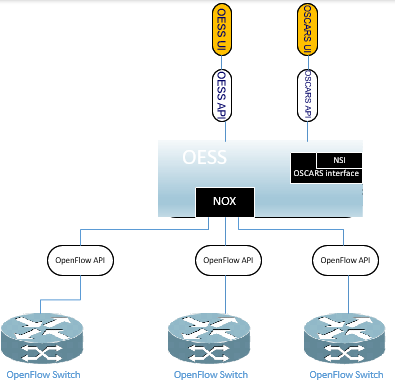
\includegraphics[width=0.6\textwidth]{figures/ControlPlane.PNG}
\caption{OESS software architecture}
\label{fig:ControlPlane}
\end{figure*}

\paragraph{OESS-OSCARS integration}
OESS includes an OSCARS interface module as shown in Fig.~\ref{fig:ControlPlane}. OESS automatically generates a
topology file for its domain and uploads it to the OSCARS
topology service as shown in Fig~\ref{fig:oscarsoess}. Only interfaces and VLAN IDs for which
users have granted OSCARS access appear in the OSCARS
topology file.

When a user requests an inter-domain circuit
via the OESS UI, the UI loads all topologies located in the
OSCARS topology service, and presents them to the user.
Once the endpoints have been selected and the user requests
that a VC be provisioned, the OESS UI submits a request to
OSCARS via the OSCARS SOAP API on behalf of the user.
At this point, the request has been turned over to OSCARS to
complete its path computation, and inform the other domains
of the request. When it is time for OSCARS to provision the
circuit in the local domain, it contacts the Path Setup Service
(PSS). When OESS is deployed in a domain, the OSCARS
PSS is replaced with the OESS PSS. The OESS PSS takes
the provisioning request from OSCARS, as shown in Fig~\ref{fig:oscarsoess}, and provisions an
OpenFlow path as described earlier. The OESS then reports the
success or failure of the provisioning procedure to OSCARS.
In cases where a user request for an inter-domain VC is sent
directly to OSCARS, the OESS PSS is nevertheless involved
to check the validity of the VC request and to carry out the
OpenFlow path provisioning.

\begin{figure}
\centering
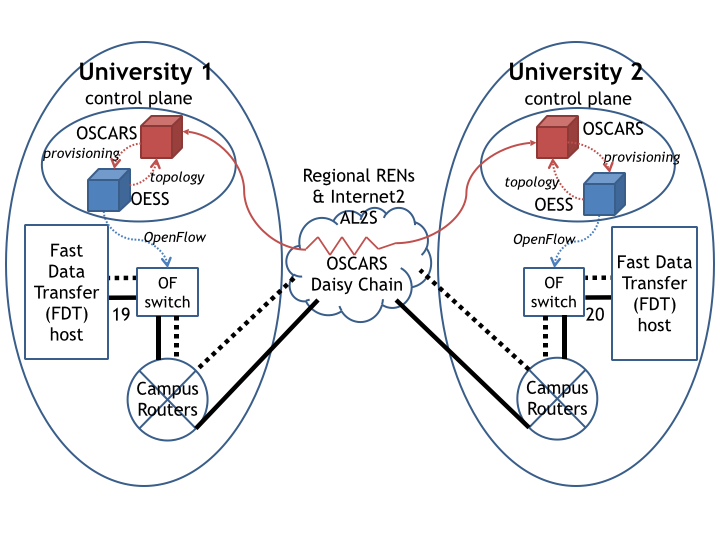
\includegraphics[width=0.6\textwidth]{figures/oscarsoess.png}
\caption{OSCARS and OESS integration}
\label{fig:oscarsoess}
\end{figure}


\section{Multi-domain SDN}
\label{sec:mdsdn}
Section~\ref{sec:multidomain-SDN-deploy-and-config} describes the equipment,
Section~\ref{sec:multidomain-SDN-path-provisioning} describes control-plane
operations for path provisioning, and Section~\ref{sec:multidomain-SDN-FDT-access} describes the actions required
in the hosts at the ends of an L2 path to support our use case (dataset transfers).
Section~\ref{sec:multidomain-SDN-data-plane-expts} describes a simple experiment
to test data-plane connectivity across the dynamically configured inter-domain L2 VLAN paths.

\subsection{Equipment}
\label{sec:multidomain-SDN-deploy-and-config}

In a project called Dynamic Network System (DYNES) \cite{1742-6596-396-4-042065}, distributed instruments were deployed in 40 universities and 11 regional RENs. Our work
used the DYNES instruments in the following universities:
(i) U. Virginia (UVA), (ii) MAX GigaPoP (MAX), (iii) U. Wisconsin, Madison (UWisc), (iv) University of New Hampshire (UNH), (v) Internet2 Lab (I2Lab), (vi) Rutgers University,  (vii) Indiana University (IU), and (viii) Colorado University (CU). These university
networks are interconnected via their corresponding regional RENs, and Internet2 Advanced Layer 2 Service (AL2S) \cite{AL2S}. Fig.~\ref{fig:network} illustrates the setup using just two university domains as an example.
\begin{figure}
\centering               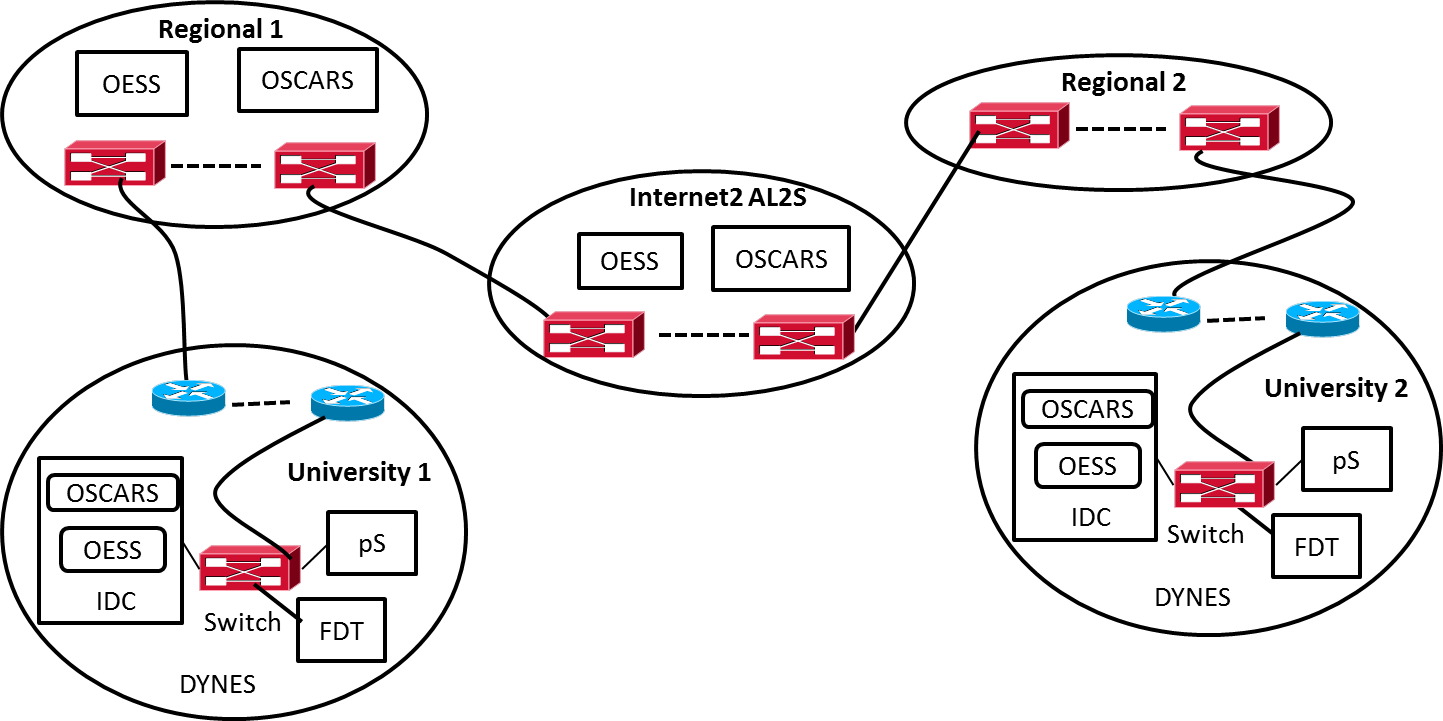
\includegraphics[width=0.7\textwidth]{figures/multi-domain-network.png}
\caption{An illustration of our multi-domain dynamic L2 path service deployment; Fast Data Transfer (FDT) server; Inter-Domain Controller (IDC); perfSONAR (pS) host; Open Exchange Software Suite (OESS); On-Demand Secure Circuits and Advance Reservation System (OSCARS); Advanced Layer 2 Service (AL2S)}
\label{fig:network}
\end{figure}

Each university
campus DYNES equipment, as shown in Fig.~\ref{fig:network},
consists of three hosts: Fast Data Transfer (FDT) server, Inter-Domain Controller (IDC) host, perfSONAR (pS) \cite{perfSONAR} host,
and one Ethernet switch (which is OpenFlow enabled in some sites). The FDT server runs data-transfer applications, the IDC host runs the control-plane software (OSCARS, and OESS at sites with an OpenFlow-enabled switch), and the pS host runs active-measurement tools for monitoring network performance.

Some regional RENs such as Regional 1 in Fig.~\ref{fig:network}
run OSCARS and OESS controllers to offer dynamic
L2 path service while others such as Regional 2 in
Fig.~\ref{fig:network} offer only static L2 path service and
hence do not deploy OESS and OSCARS.
As can be expected with the roll-out of a new networking
service, organizations will slowly deploy the service
one-at-a-time. Static L2 path service is available from most RENs
and university campus networks, and can be used to bridge gaps in the
dynamic L2 service offering.

Internet2's Advanced Layer-2 Service (AL2S) network has 39 OpenFlow-enabled
Ethernet switches, as shown in Fig~\ref{fig:AL2S}, and is operated in L2 Virtual LAN (VLAN) mode.
AL2S delivers a strategic advantage for leaders in research and education (R$\&$E) by providing effective and efficient wide area 100 gigabit Ethernet technology. AL2S allows users to create their own VLANs on the Internet2 AL2S backbone. Static or Dynamic, point-to-point or multipoint, intra-domain or inter-domain, AL2S puts control of the backbone VLANs into the users' hands for the creation of purpose-built private circuits using infrastructure already in place. AL2S is available to 279 higher education institutions include Univeristy of Virginia. AL2S uses OESS for controlling the OpenFlow switches, and OSCARS for inter-domain L2 paths.
\begin{figure*}[htbp!]
\centering 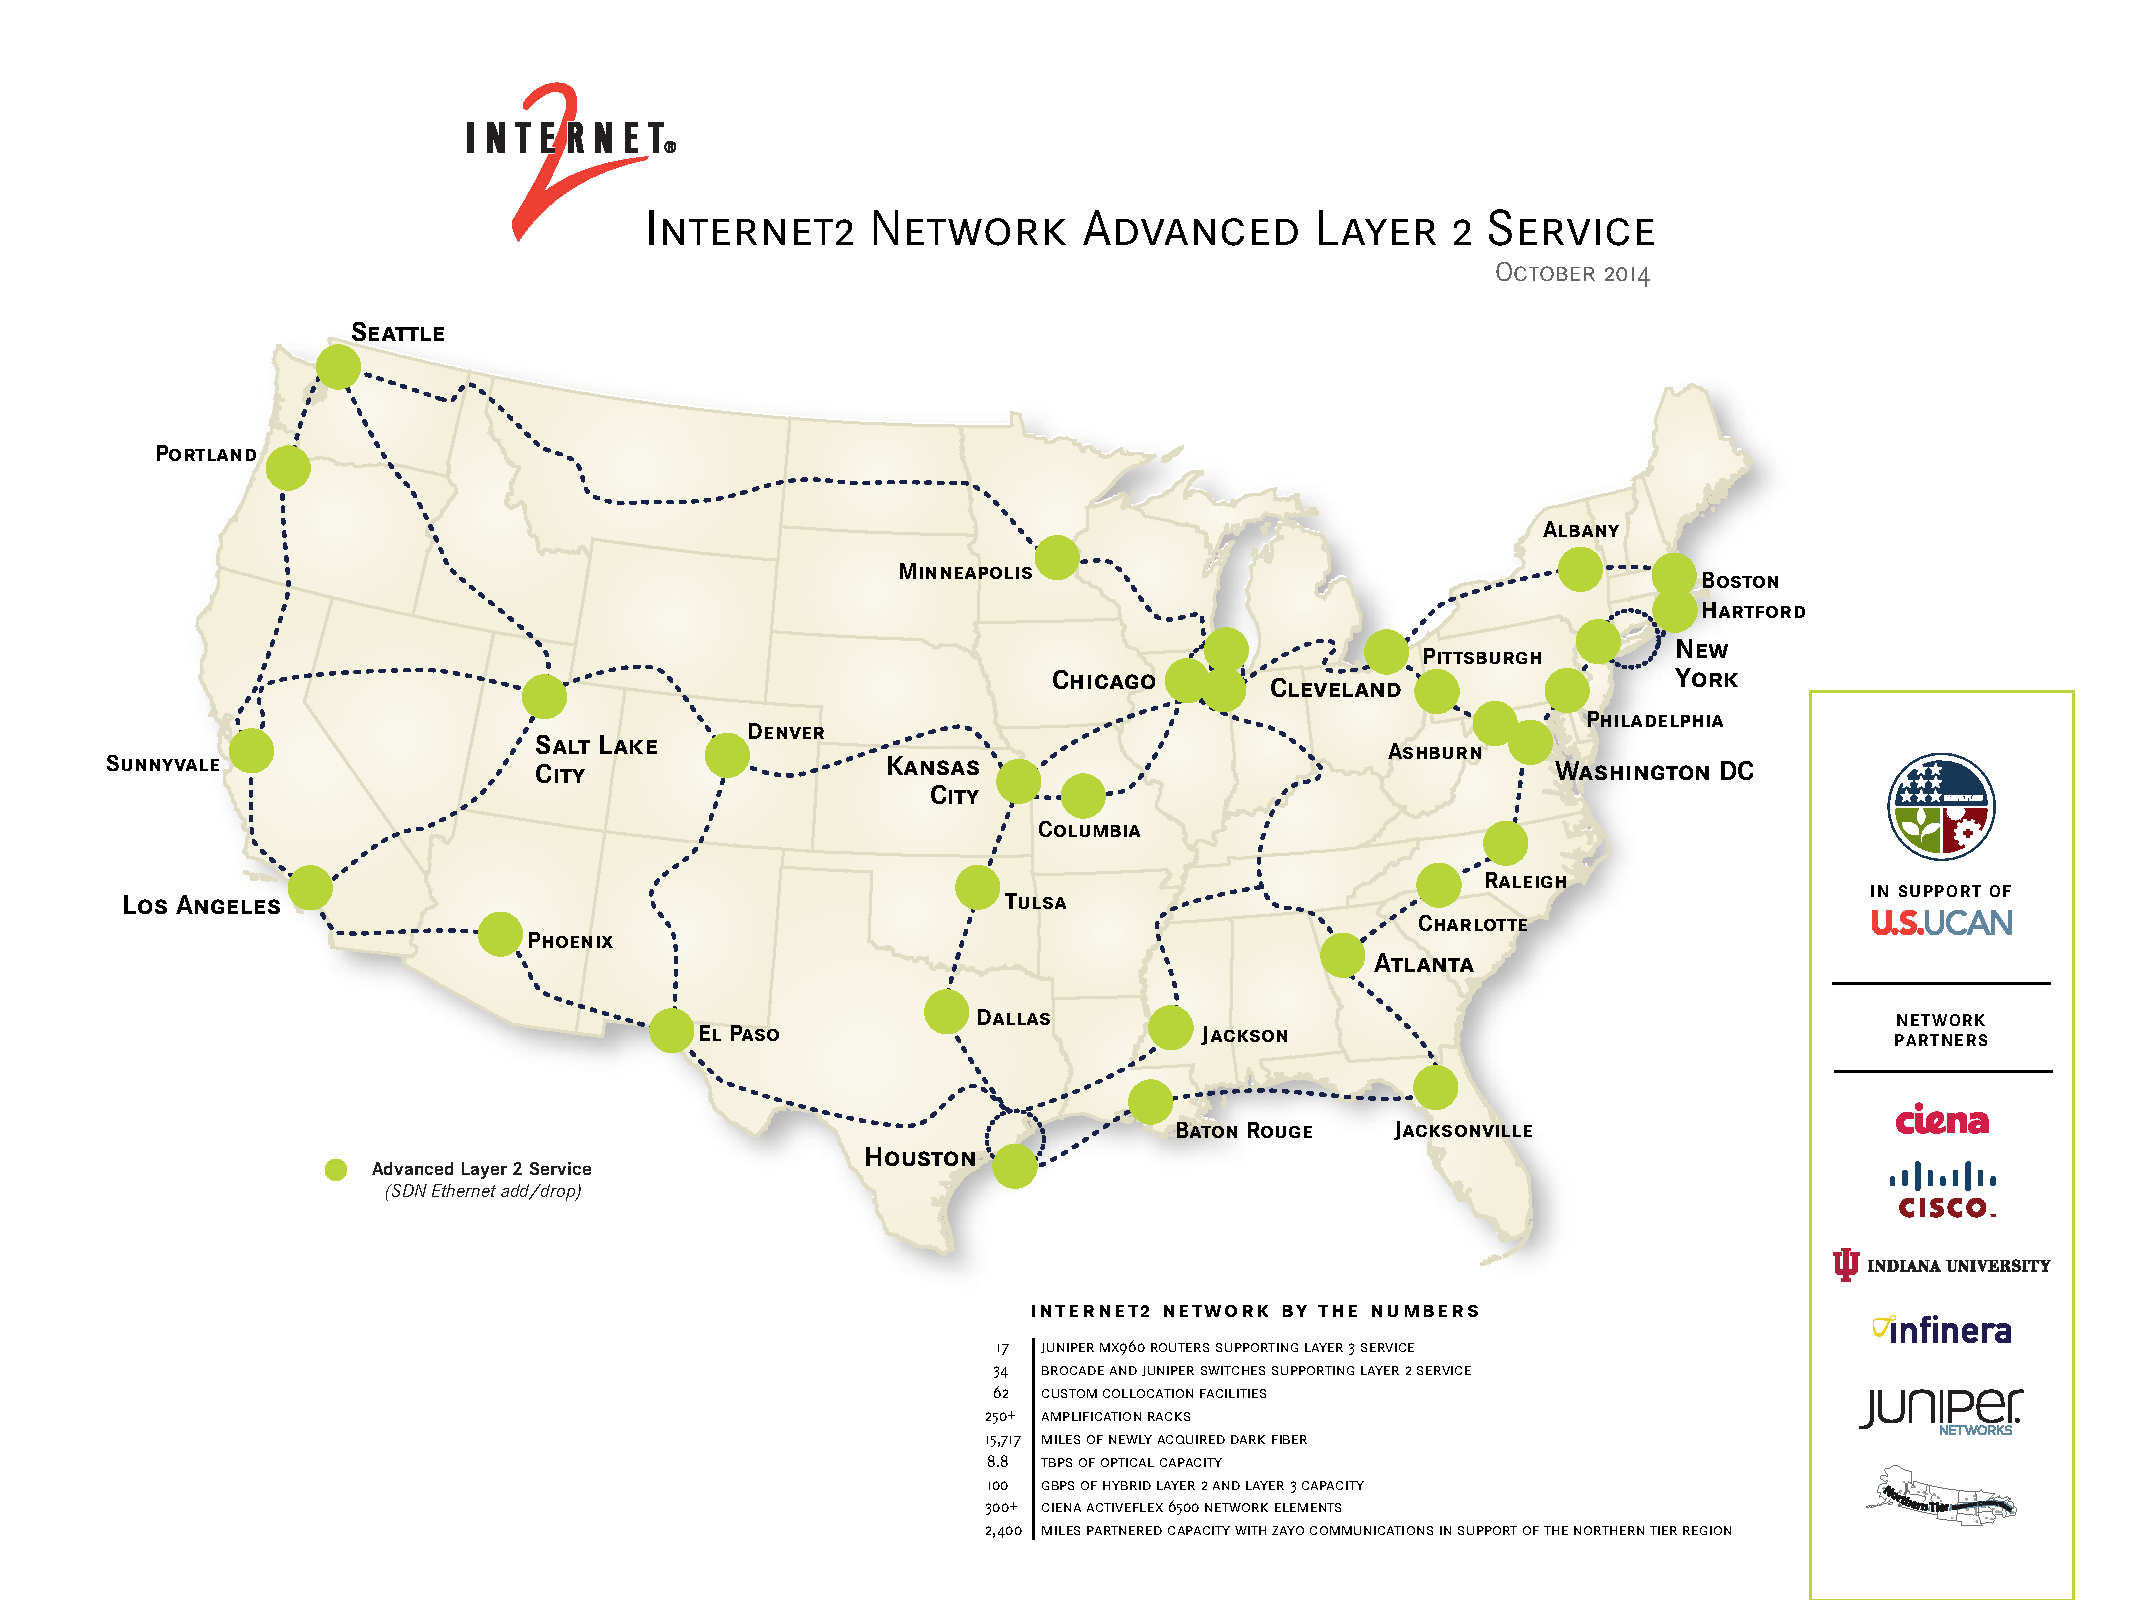
\includegraphics[width=0.80\textwidth]{figures/AL2S.pdf}
\caption{Internet2 Advanced Layer 2 Service (AL2S) Network}
\label{fig:AL2S}
\end{figure*}

We \emph{first} describe how the
DYNES equipment was configured at each site.
\emph{Next}, we describe the actions needed within campuses between the
location of the DYNES equipment and the campus edge. \emph{Finally},
we describe the actions required from regional RENs
that did not deploy this dynamic L2 path service.

\textbf{Step 1.} At each DYNES site, we logged in to the OpenFlow
enabled switch, configured the IP address of the IDC host
on which the OESS (OpenFlow controller) is being run, and
added the set of ports to be controlled by the OESS into
the switch's OpenFlow instance (only one instance is used).
The OpenFlow switch models used by the DYNES project
support \emph{hybrid-switch} mode in which OpenFlow controlled
and traditionally configured ports can co-exist on the switch.
However, these switches do not support \emph{hybrid-port} mode in
which each individual port can be controlled by both the
OpenFlow controller and traditional configuration methods.

The next set of operations at each DYNES site consisted of
(i) initiating OESS and OSCARS on the IDC host, (ii) providing the OESS with the switch's control-port IP address,
and (iii) configuring OESS and OSCARS through their Web
UIs. Specifically, the OESS UI is used to set the remote-link
information for the data-plane port of the peering network.
For example, the UVA DYNES switch port 1 is connected
to say port 1 of a UVA campus router. A static VLAN was
configured from port 1 of this UVA campus router through
the other UVA campus routers, and through the regional
REN (MARIA) routers to the MARIA router port that is
connected to port et-3/0/0.0 on the Internet2 AL2S switch
in Ashburn, VA. This static VLAN serves as the remote
link between UVA DYNES network and Internet2 AL2S.
Information about this remote link is entered into the UVA
DYNES OESS to identify the peering domain, node, and
port. The counterpart action was performed at Internet2's
OESS for the UVA DYNES switch remote link. This remote-link information was provided manually to Internet2. The
OESS UI is also used to configure the set of allowed VLANs
on each port of the DYNES switch.

UVA DYNES OSCARS needed to be configured with a server certificate, and the certificate owner and issuer information needed to be manually communicated to Internet2's administrator for configuration of Internet2's AL2S OSCARS. These certificates are used in the authentication
process for inter-domain L2 path requests.

\textbf{Step 2.} Most of the involved campus networks and regional
RENs support static L2 path services. This allowed us to request and obtain provisioned L2 paths with a specified set of
VLAN IDs from campus network administrators. These L2
paths cut across the campus switches/routers between the
DYNES equipment and the campus edge router. Having the
capability to establish static L2 paths allows for a gradual
introduction of OpenFlow switches under OESS control into
campus networks.

\textbf{Step 3.} Similarly, we contacted regional REN administrators to obtain static L2 paths with specified VLAN IDs
across their networks to Internet2. Again this capability of using static L2 paths allows for a gradual addition of
dynamic L2 path service by different regionals at different
times, and yet support dynamically created end-to-end L2
paths.

The above experience shows the various steps required to
configure OSCARS and OESS in each organization that is
ready to support dynamic L2 service, as well as the feasibility of using static L2 paths through networks whose organizations are not as-yet ready for the dynamic service.

\subsection{Path/VLAN provisioning through switches}
\label{sec:multidomain-SDN-path-provisioning}

This section describes the process of establishing a new VLAN via the OESS UI \cite{OESS}. We use the term ``path'' if the VLAN has just two
endpoints, and the term ``multipoint VLAN'' if there are multiple endpoints.

After user authentication in the OESS UI through the login process, the OSCARS IDC workgroup should
be selected. Then in the Actions tab, the user should select the \texttt{Create a New VLAN} option. The system then guides the user through a 6-step procedure to provision a VLAN.

\paragraph{Step 1:  Basic characteristics}
Fig.~\ref{fig:oessbasic} shows a screenshot of the first step for a local circuit, and Fig.~\ref{fig:oessbasic-interdomain} shows a screenshot of the first step for an inter-domain circuit.
In both cases, the user should enter a human-readable name for the VLAN being created in the
\texttt{Description} field. For inter-domain paths, the user is offered the option of specifying
bandwidth for the circuit (see Fig.~\ref{fig:oessbasic-interdomain}), but not for intra-domain (local) paths (see Fig.~\ref{fig:oessbasic}).
 If the user wants a failed VLAN that had been automatically routed to a backup path to be restored to the primary path, the \texttt{Restore to Primary} field should be enabled. If the VLAN can stay routed on the backup path, this field can left in the \texttt{Off} state. The \texttt{Multipoint Static MAC Routing} field allows a user to associate a destination MAC addresses with each endpoint of a multipoint VLAN. Packets destined to such a configured MAC address will be forwarded to only the corresponding endpoint rather than to all endpoints as would happen if this feature was left disabled, or for packets with destination MAC addresses that were not attached to any endpoints of the multipoint VLAN.
 This field is only offered for local (intra-domain) paths (see Fig.~\ref{fig:oessbasic}), and
 not for inter-domain paths (see Fig.~\ref{fig:oessbasic-interdomain}). The \texttt{Type of Circuit} field should be set by the user to \texttt{Local}, if the VLAN traverses the single domain controlled by the particular OESS whose UI is being accessed. If the VLAN will
need to traverse multiple domains, the user should select the \texttt{Interdomain} option. This
option will cause the OESS to obtain all accessible endpoints from the
OSCARS topology service as described in Section~\ref{sec:OESS}, and load these into the UI in the next step for endpoint selection.

\begin{figure}[htb!]
\centering
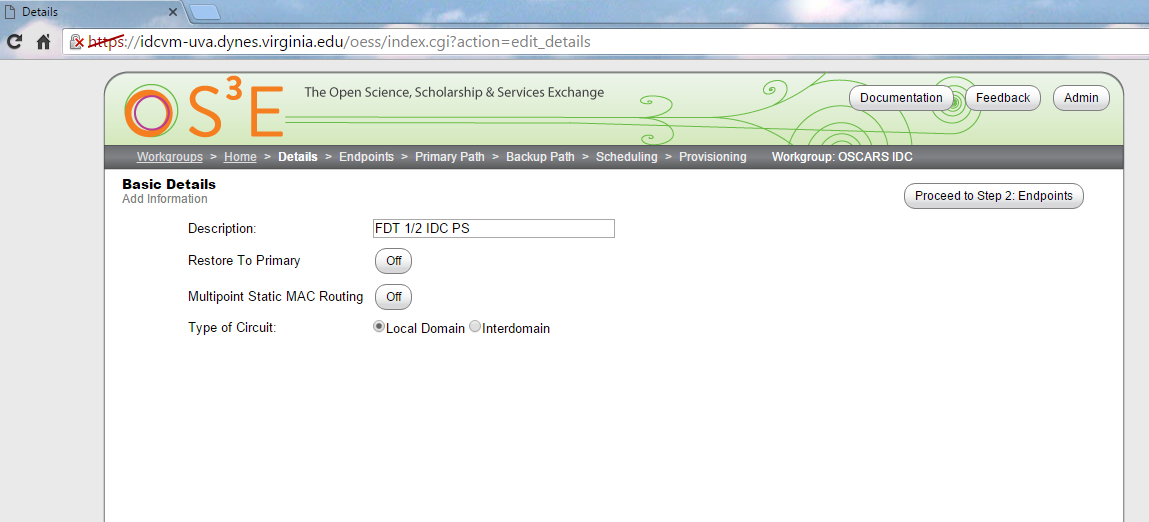
\includegraphics[width=0.8\textwidth]{figures/oess-basic.png}
\caption{OESS UI Step 1: Choose basic characteristics for an intra-domain path}
\label{fig:oessbasic}
\end{figure}

\begin{figure}[htb!]
\centering
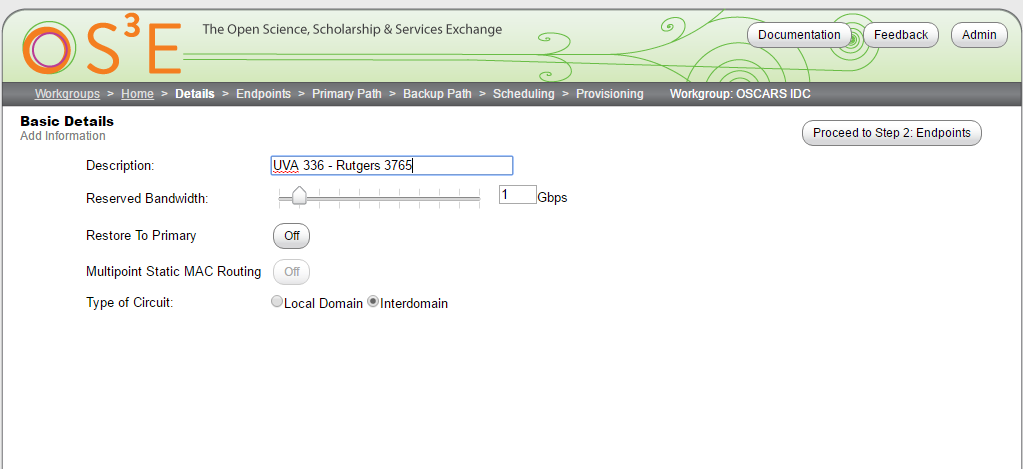
\includegraphics[width=0.8\textwidth]{figures/oess-basic2.png}
\caption{OESS UI Step 1: Choose basic characteristics for an inter-domain path}
\label{fig:oessbasic-interdomain}
\end{figure}



\paragraph{Step 2: Endpoints and VLAN IDs}
Fig.~\ref{fig:oesspoints} shows Step 2, in which the user selects the endpoints of the VLAN.
For each endpoint, the user needs to provide a corresponding VLAN ID. The user starts by clicking on the dot in the map displayed on the screen. In this example, the single dot represents the UVA DYNES switch. Since the \texttt{Type of Circuit} field was set to \texttt{Local} in Step 1,
OESS displays just the seven endpoints of the UVA DYNES network (on the bottom right corner). Specifically, these endpoints are ports on the single UVA DYNES switch served by the OESS being used for this provisioning process. When the user clicks on a port that should be an endpoint in the VLAN, OESS displays a window in which the user is required to provide a specific VLAN ID. Each workgroup is provided rights to use specific VLAN IDs for each endpoint. Hence
authorization is run by OESS allows before a particular VLAN ID is used for provisioning. In this
example, the user has selected four interfaces, specifically ports 0/19, 0/24, 0/22, and 0/20,
of the UVA DYNE switch,
and hence these interfaces are displayed under \texttt{Endpoints} in the main part of the screen.
The user has selected the same VLAN ID 332 for all four endpoints.
\begin{figure}[htb!]
\centering
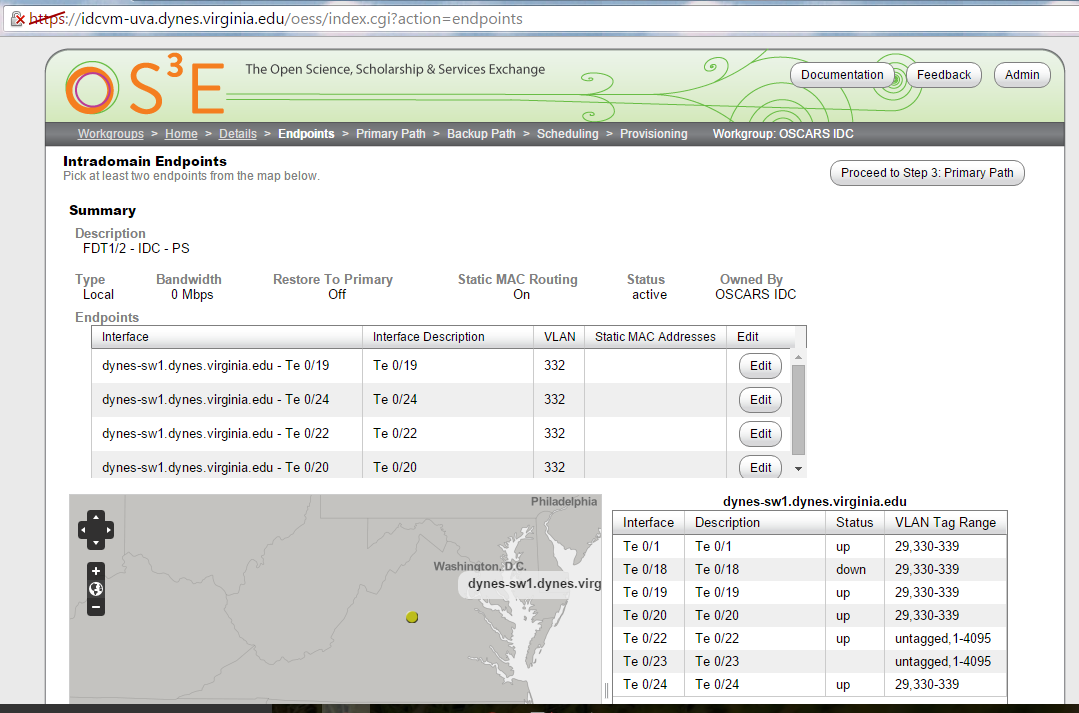
\includegraphics[width=0.8\textwidth]{figures/oess-points.png}
\caption{OESS UI Step 2: Selection of endpoints and VLAN IDs}
\label{fig:oesspoints}
\end{figure}

\paragraph{Step 3: Select primary path}
Fig.~\ref{fig:oessprimary} shows the OESS UI screenshot for Step 3 in which the user can select a path or ask OESS to suggest the shortest path. If a user is not particular about the selected path, users can click on the\texttt{ Suggest Shortest Path} button, and OESS will find the shortest path between the selected endpoints. Alternatively, a users can click on links to add or remove them from a path. The path must connect the endpoints and must not have any loops. For the example show, since the three interfaces are on the same UVA DYNES switch, there is only one possible multipoint VLAN.
\begin{figure}[htb!]
\centering
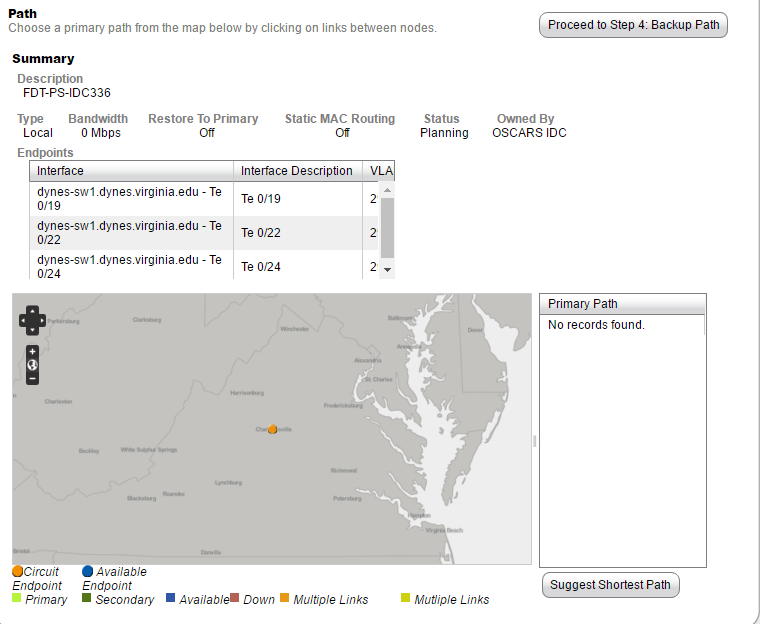
\includegraphics[width=0.8\textwidth]{figures/oess-primary.png}
\caption{OESS UI Step 3: Primary path selection}
\label{fig:oessprimary}
\end{figure}

\textbf{Step 4: Select backup path}
In Step 4, a user can select a backup path for automatic switch-over from the primary path in case of
failures. If the user clicks on the \texttt{Suggest Shortest Path} button, the OESS will attempt to find an path that has minimal overlap with the primary path.  Selection of a backup path is optional. Fig.~\ref{fig:oessbackup} shows a screenshot of the OESS UI Step 4.
\begin{figure}[htb!]
\centering
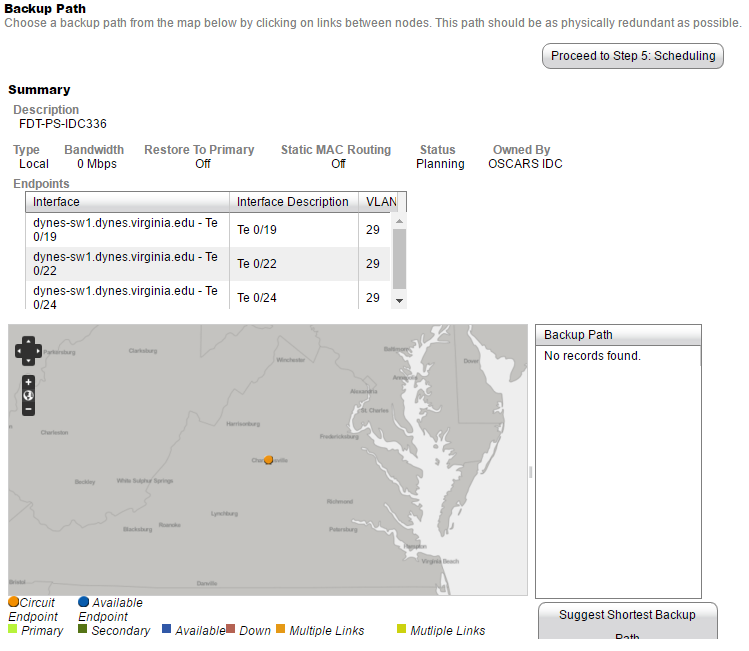
\includegraphics[width=0.8\textwidth]{figures/oess-backup.png}
\caption{OESS UI Step 4: Backup path selection}
\label{fig:oessbackup}
\end{figure}

\textbf{Step 5: Scheduling}
\begin{figure}[htb!]
\centering
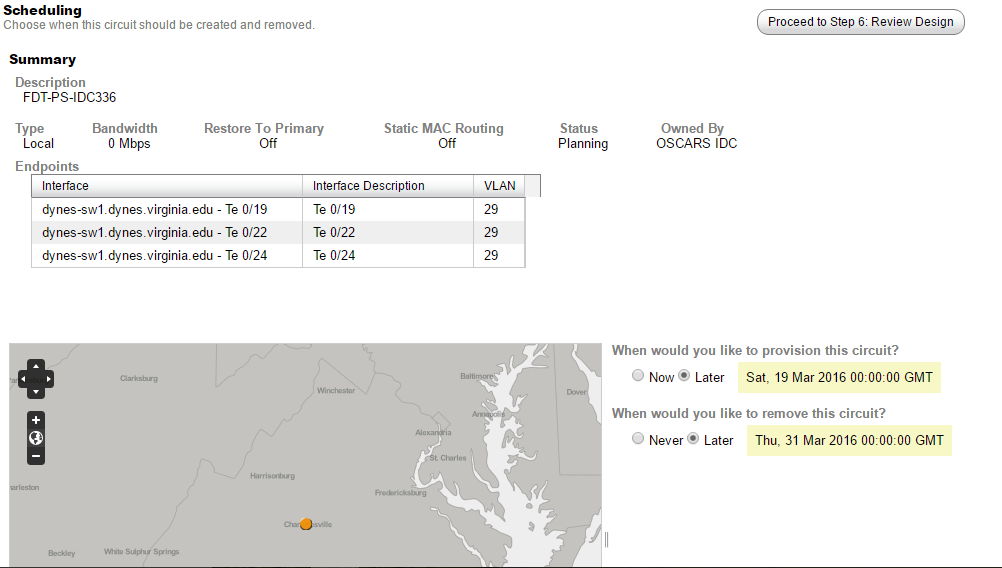
\includegraphics[width=0.8\textwidth]{figures/oess-schedule.png}
\caption{OESS UI Step 5: Circuit scheduling}
\label{fig:oessschedule}
\end{figure}
Fig.~\ref{fig:oessschedule} shows a screenshot of the OESS UI Step 5, in which a user can specify
a start time and release time for the circuit. In the example shown, the user
has requested a later
start time (not ``now''), and has specified a particular future date when the circuit should be released.

\paragraph{Step 6: Review design and submit circuit request}
Users are given an opportunity to review the design before selecting
the \texttt{Submit Circuit Request}.
Fig.~\ref{fig:oessreview} shows the corresponding OESS UI screenshot.
\begin{figure}[htb!]
\centering
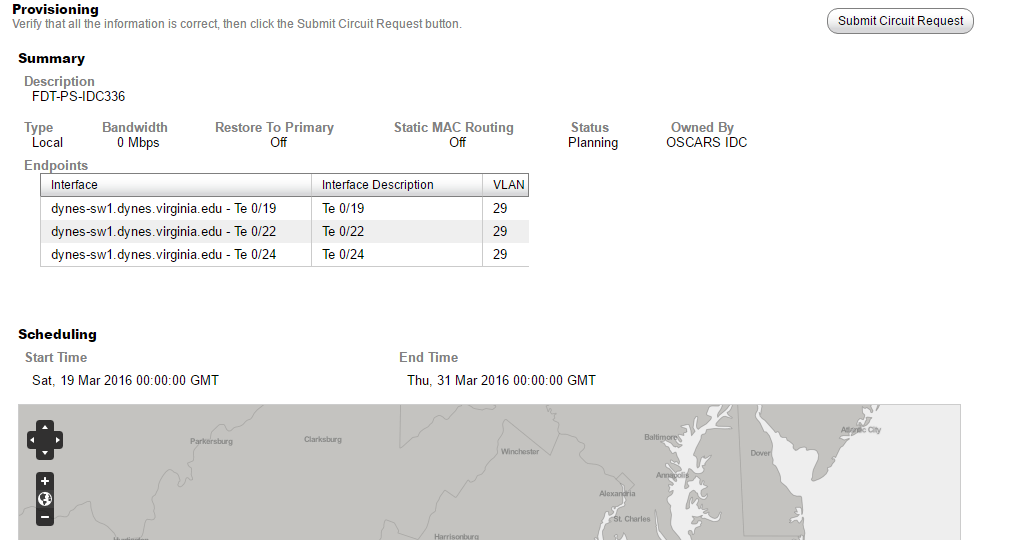
\includegraphics[width=0.8\textwidth]{figures/oess-review.png}
\caption{OESS UI Step 6: Review design}
\label{fig:oessreview}
\end{figure}

If the OESS is successful in setting up the circuit between the selected endpoints
at the specified rate, in the time interval specified in Step 4, a success message
is displayed to the user through the UI. If not, a failure message is displayed.
One of the drawbacks of the current software is that failure messages do
not offer a cause for the failure.

\subsection{Path Configuration at Hosts}
\label{sec:multidomain-SDN-FDT-access}
Three steps are required to configure the FDT hosts at the
ends of an L2 path: (i) a VLAN with the appropriate VLAN
ID is configured on the FDT NIC that is connected to the
DYNES switch, (ii) IP addresses on the same subnet are
assigned to the VLANs configured at the two FDT hosts,
and (iii) the traffic control (\texttt{tc}) Linux utility is configured
to rate limit outgoing traffic to the L2-path rate used in the
path-reservation phase.
\begin{figure}
\centering
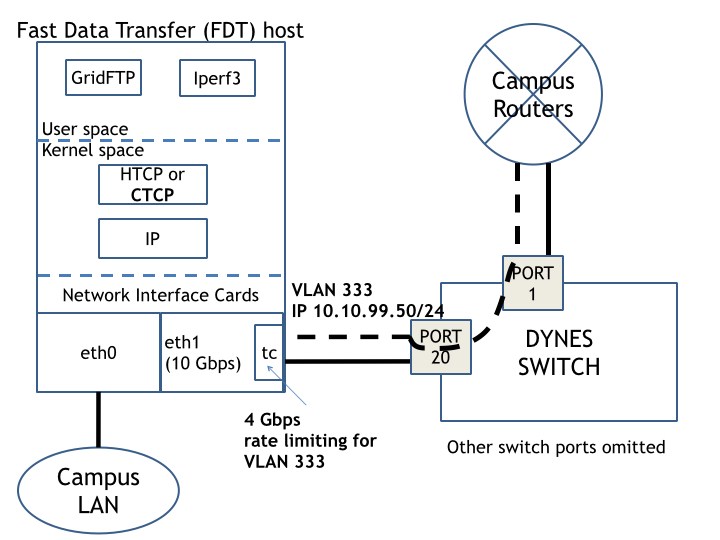
\includegraphics[width=0.6\textwidth]{figures/uvadynes.png}
\caption{Configuring the Fast Data Transfer (FDT) host for the L2 path}
\label{fig:uvadynes}
\end{figure}

Fig.~\ref{fig:uvadynes} illustrates the UVA DYNES data-plane with a configured VLAN for the end-to-end L2 path to the IU FDT.
However before discussing the details of Fig.~\ref{fig:uvadynes}, recall the example end-to-end L2 path described in Fig.~\ref{fig:AL2S} between
port 19 of the DYNES switch in the University 1 network,
and port 20 of the DYNES switch in the University 2 network of Fig.~\ref{fig:AL2S}. While the endpoints specified in the request
to the OESS are the two switch ports, the L2 path essentially
extends between the FDTs at University 1 and University 2
as the specified switch ports are connected to the FDTs.

Therefore, the VLAN ID used on the interface from the FDT
to the DYNES switch in the request to the OESS needs to
now be configured in the FDT. In the example shown in
Fig.~\ref{fig:uvadynes}, the VLAN ID used in the request to the OESS for
port 20 of the UVA DYNES switch for the L2 path to the
IU FDT was 333. Now, using the Linux \texttt{vconfig} command
in the UVA FDT, the user or application needs to configure
VLAN 333 on the \texttt{eth1} NIC, which is the one connected to
port 20 of the DYNES switch.

The second step that needs to be executed on the FDT is a
configuration of an IP address associated with the newly created VLAN. For this purpose the Linux \texttt{ifconfig} command
is used. Fig.~\ref{fig:uvadynes}shows that private IP address 10.10.99.50
is assigned to VLAN 333 on \texttt{eth1}. IP packets sent out
with source IP address equal to 10.10.99.50 will be carried
in tagged Ethernet frame headers with VLAN ID set to 333.

Fig.~\ref{fig:uvadynes} also shows that the FDT host has another NIC, \texttt{eth0}
for connectivity to the campus LAN. This interface for logging into the FDT remotely using an ssh client.

The reason for needing to configure IP on the VLAN is to allow for the usage of existing applications, such as GridFTP
and \texttt{nuttcp}, and transport-layer protocols such as HTCP \cite{HTCP}
as illustrated inside the FDT in Fig.~\ref{fig:uvadynes}. Packets sent on the
end-to-end L2 path are not subject to L3 (IP) header based
packet forwarding because all switches on the path have
been provisioned to execute packet forwarding based on the
VLAN ID. IP headers are nevertheless included/extracted at
the FDT servers because of the applications' use of TCP/IP
sockets.

Furthermore, the private IP addresses configured for the
FDT VLANs at the two ends need to belong to the same
subnet to avoid having to add destination-specific routes to
the IP-routing table in the FDTs. For this L2 path, the
VLAN ID used on the port of the IU DYNES switch was
2399 and the IP address assigned to VLAN 2399 on the
Ethernet NIC in the IU FDT host was 10.10.99.40.

In our usage of these L2 paths,
we manually executed these VLAN and IP address configuration commands at the FDT hosts, having procured privileged access for the execution of these commands. However, for general-purpose use of L2 path-based networking, applications should be integrated (through shell scripts or with
modifications) with a signaling-client module that issues requests for paths to OESS, handles responses, and additionally configures VLANs and IP addresses at the FDTs. Further, an end-to-end session protocol is required to exchange
subnet identifier/mask information to ensure that the private IP addresses assigned to the VLANs at the two end
FDTs match. Since the FDT and IDC servers have multiple Ethernet interfaces, one of which is connected to the campus IP-routed
infrastructure, e.g., \texttt{eth0} in the FDT shown in Fig.~\ref{fig:uvadynes}, L3 IP
service is used for all signaling messages.

Finally, Fig.~\ref{fig:uvadynes} shows that the Linux \texttt{tc} utility is used in the
FDT host to limit the rate at which the 10Gbps \texttt{eth1} NIC
transmits frames. The example VLAN shown was created
with a 3 Gbps rate request; therefore, \texttt{tc} would have been
configured to rate limit VLAN-333 Ethernet frames to 3
Gbps.

\subsection{Data plane Experiments}
\label{sec:multidomain-SDN-data-plane-expts}

This section describes the methodology used to test a newly provisioned VLAN.
It not only verifies that the VLAN has been successfully provisioned across the network(s), 
but also verifies the configuration actions at the end hosts.
\begin{figure}[htb!]
\centering
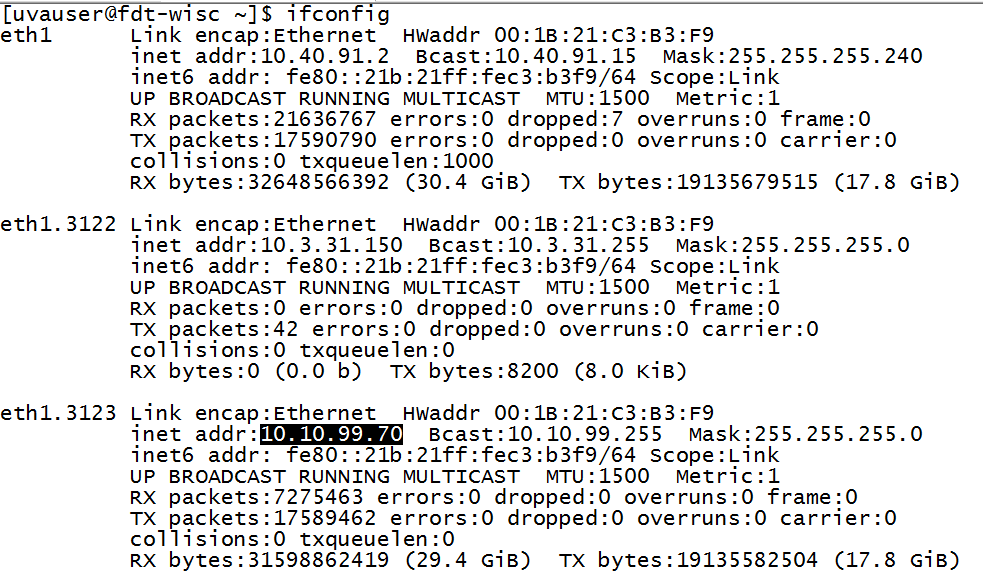
\includegraphics[width=0.8\textwidth]{figures/ifconfig.png}
\caption{Linux utility \texttt{ifconfig}}
\label{fig:ifconfig}
\end{figure}
An interdomain circuit was configured from the FDT at UWisc to the FDT at UVA. The VLAN ID
at the UWisc FDT was 3123, and at the UVA FDT, it was 336. The IP addresses/subnet masks 10.10.99.70/24 and 10.10.99.50/24 were assigned to the UWisc FDT VLAN and UVA FDT VLAN,
respectively.

Before running an end-to-end data-plane test, the Linux utility \texttt{ifconfig} was used to check the configuration of the VLANs at both ends. Fig.~\ref{fig:ifconfig} shows the UWisc interface \texttt{eth1} was configured with a VLAN with ID 3123, and this VLAN was
 assigned IP address 10.10.99.70 with subnet mask /24.

Next, the \texttt{ping} command was executed to test the reachability across this newly configured VLAN path from UWisc FDT to UVA FDT.
 Fig.~\ref{fig:ping} shows that the UVA FDT VLAN was reachable from the UWisc FDT,
 as the latter receives a reply to the ping command sent to IP address 10.10.99.50, which is
 the address that was assigned to VLAN 336 at the UVA FDT interface. Success of this
\texttt{ping} execution verifies that the L2 path was successfully setup across all five domains,
UWisc, CIC OmniPoP (regional REN for UWisc), Internet2 AL2S, MARIA (regional REN for UVA),
and UVA. Further it attests to the successful configuration of the two end hosts.

\begin{figure}[htb!]
\centering
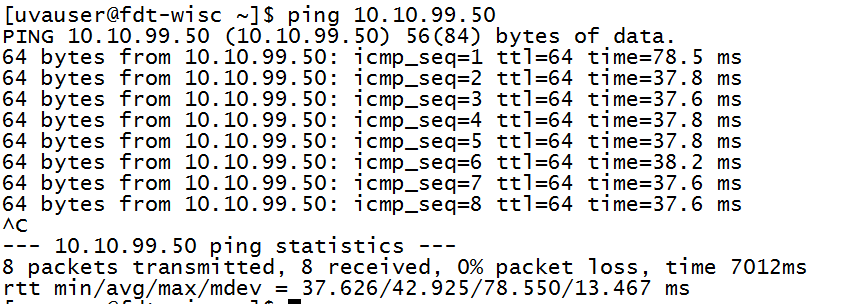
\includegraphics[width=0.8\textwidth]{figures/ping.png}
\caption{Linux utility ping}
\label{fig:ping}
\end{figure}



\section{Insights Gained}
\label{sec:insights}

Section~\ref{sec:config-ovhd} describes the configuration
overhead required to run this dynamic L2 path service, and addresses
the question of scalability.
Section~\ref{sec:ckt-provisioning} describes
our experience as users of OSCARS and OESS in configuring
inter-domain L2 paths.
Finally, Section~\ref{sec:other-challenges} describes
other challenges we faced in the course of this deployment.

\subsection{Configuration Overhead and Scalability}
\label{sec:config-ovhd}
A number of administrator
actions are required to configure the OpenFlow switches, OESS and OSCARS. The
larger the number of such required actions, the greater the
potential for administrator errors.
Effort is required to reduce the number of required administrator
actions wherever possible.

To achieve a global-scale dynamic L2 path-service deployment,
the current solution for making available endpoint information
through the OESS Web user interface to allow for user selection of path endpoints
needs
to be changed. A potential solution for allowing users to find the
endpoint identifiers for hosts that support dynamic L2 path service is
to incorporate this service into the widely deployed DNS system. If a user
has the domain name of a host that supports dynamic L2 path service, a new DNS
resource record could provide the translation of this name to the endpoint
identifier required by OESS and OSCARS.

Finally, the scalability and usability of the pS Topology Service should be assessed.
As described in Section~\ref{sec:control-plane}, the OSCARS topology service
pushes the topology of a domain to the pS Topology Service, allowing OSCARS
in other domains to request topology information when needed. While this open
topology sharing approach works in the REN community, it is not suitable
for commercial providers. Contrast this approach to the more practical Border Gateway Protocol solution of sharing only address reachability across domains.
Therefore, this part of the OSCARS design needs to be revisited.


\subsection{Path Provisioning and Testing}
\label{sec:ckt-provisioning}

The OESS and OSCARS software systems were relatively stable and their Web user interfaces were fairly easy to navigate. In general, these controllers are
robust and allowed us to set up and tear down inter-domain paths dynamically.
However, three aspects need improvement: error reporting, path setup delay,
and path failure debugging.

The error reporting functionality of OSCARS needs to be enhanced. Path setup failures
occur due to a lack of bandwidth, unavailability of a requested VLAN ID, or due to an expired certificate. In all these cases, while OSCARS reports a failed setup attempt,
the error messages are cryptic and do not offer users a decipherable reason for the failure.

The second issue relates to setup delay and the OSCARS approach of handling only one path setup at a time.
In particular, a failed path setup attempt causes OSCARS to wait for a user-configured timeout interval, which is currently set to 15 min. While this solution is sufficient for low call arrival rates, a programmatic test with multiple path setup-and-release attempts experienced excessive delays.

Finally, the lack of L2 connectivity tools comparable to L3 tools such as \texttt{ping} and \texttt{traceroute} made it difficult to identify the domain in which the L2 connectivity
was broken.
We used three methods to debug such connectivity issues. First, we had campus and regional REN administrators configure a specified private IP address to a specified VLAN on the port of their domain's edge router that is connected to the next domain (toward Internet2). This allowed us to use L3 tools
to verify that static VLANs across each domain were operational. Second, we used observatory hosts located at Internet2 PoPs whose ports (with specified VLANs) were made available by Internet2 to DYNES users for L2 path testing. This allowed us to create dynamic L2 paths between each campus DYNES switch and an observatory host's Internet2 router port for single campus-and-regional segment testing. Finally, we used GRNOC's routerproxy tool \cite{routerproxy} to observe packet counts at router ports while sending data between campus FDTs on configured VLANs to localize problems. These methods are rudimentary and suitable for the REN community,
but better methods leveraging OpenFlow features need to be developed.

\subsection{Other Challenges}
\label{sec:other-challenges}
In the course of one year, we experienced software upgrades to OSCARS,
X.509 certificate expirations, and even network connectivity changes (regional networks
were moved to AL2S from ION for their Internet2 access). Each of
these changes required corresponding administrative actions, sometimes in several
DYNES sites and Internet2. For example, OSCARS server peerings and topology
files had to be updated
when a regional moved its access link from Internet2's Interoperable On-demand Network (ION) to AL2S.






\section{Multi-point VLAN}
\label{sec:mdvlan}

Section~\ref{sec:multipoint-control-plane} describes the procedure
for configuring a multipoint VLAN, and Section~\ref{sec:multipoint-data-plane}
describes a data-plane experiment executed to verify successful provisioning
of the multipoint VLAN.

\subsection{Control Plane Setup}
\label{sec:multipoint-control-plane}

A multipoint VLAN can be created by OESS. However, OSCARS, which is the SDN controller
used for inter-domain circuits, does not support multipoint VLANs. Therefore, we designed
a two-step approach for creating inter-domain multipoint VLANs.

In the \emph{first} step, a point-to-point VLAN was created from the FDT host on each campus, through
the university's regional network, to the corresponding AL2S switch interface. On each campus, the VLAN was configured across the DYNES switch via the corresponding OESS controller. Since
the OESS controller on a campus only controls the DYNES (OpenFlow) switch
and not the remaining campus switches, a campus network administrator was contacted
and asked to provision the VLAN across the remaining campus switches. Since typically
these deployed campus switches are not OpenFlow capable, administrators
either login to each switch to configure VLANs, or use network management tools if available. Similarly, administrators at regional networks were contacted to provision the VLAN through
their switches.

As an example, Fig.~\ref{fig:UVA-VLAN336} shows VLAN 336 that
was provisioned across the UVA DYNES switch using OESS, through the campus switches by
a UVA campus network administrator, and across the MARIA regional network by a MARIA
administrator. The provisioned VLAN 336 terminates on port et-3/0/0.0 of the Internet2 AL2S Ashburn switch as shown in Fig.~\ref{fig:UVA-VLAN336}.
\begin{figure}[htb!]
\centering
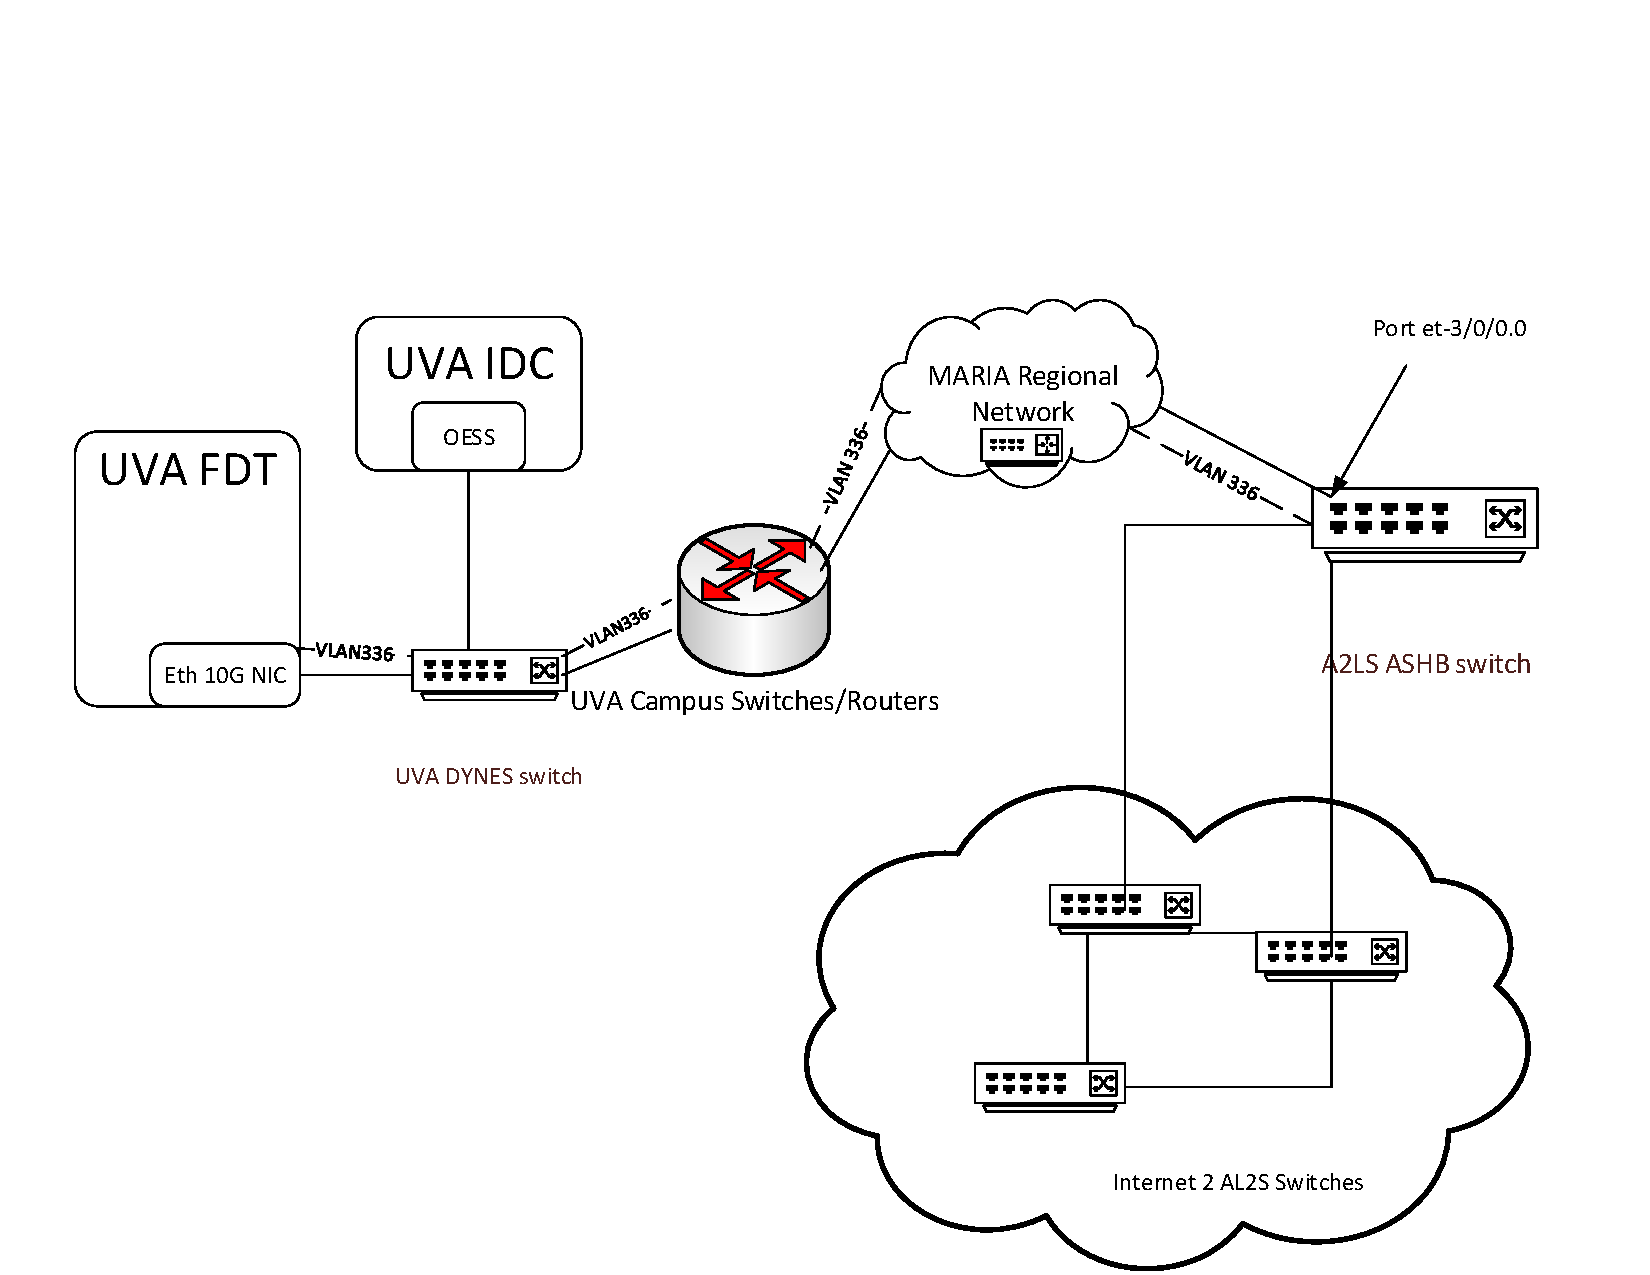
\includegraphics[width=0.8\textwidth]{figures/UVA-ASHB.pdf}
\caption{UVA DYNES - UVA campus – MARIA- ASHB}
\label{fig:UVA-VLAN336}
\end{figure}

One such provisioned VLAN was established from each campus FDT to a specific
port of an Internet2 AL2S switch. Since campus network and regional network
administrators assign VLANs for many purposes, it is unlikely to obtain the
same VLAN ID for all campus/regional networks. Already, there is some constraint
in that each campus administrator has to collaborate with the corresponding
regional network administrator to select a common range of VLANs that is still available
for allocation. One or more VLAN IDs from this range is then used in the
above-described manual provisioning process. Therefore,
the VLAN ID selected by each campus/regional network on the multipoint VLAN
could be different. This was the case for the three-point VLAN illustrated
in Fig.~\ref{fig:wanmulticast}. The VLAN ID used for the UVA-MARIA path was 336,
the VLAN ID used for the MAX path (MAX is a regional network, and hence there
is no corresponding university campus) was 1830, and the VLAN ID on the IU-Indiana
GigaPoP path was 2399.
\begin{figure}[htb!]
\centering
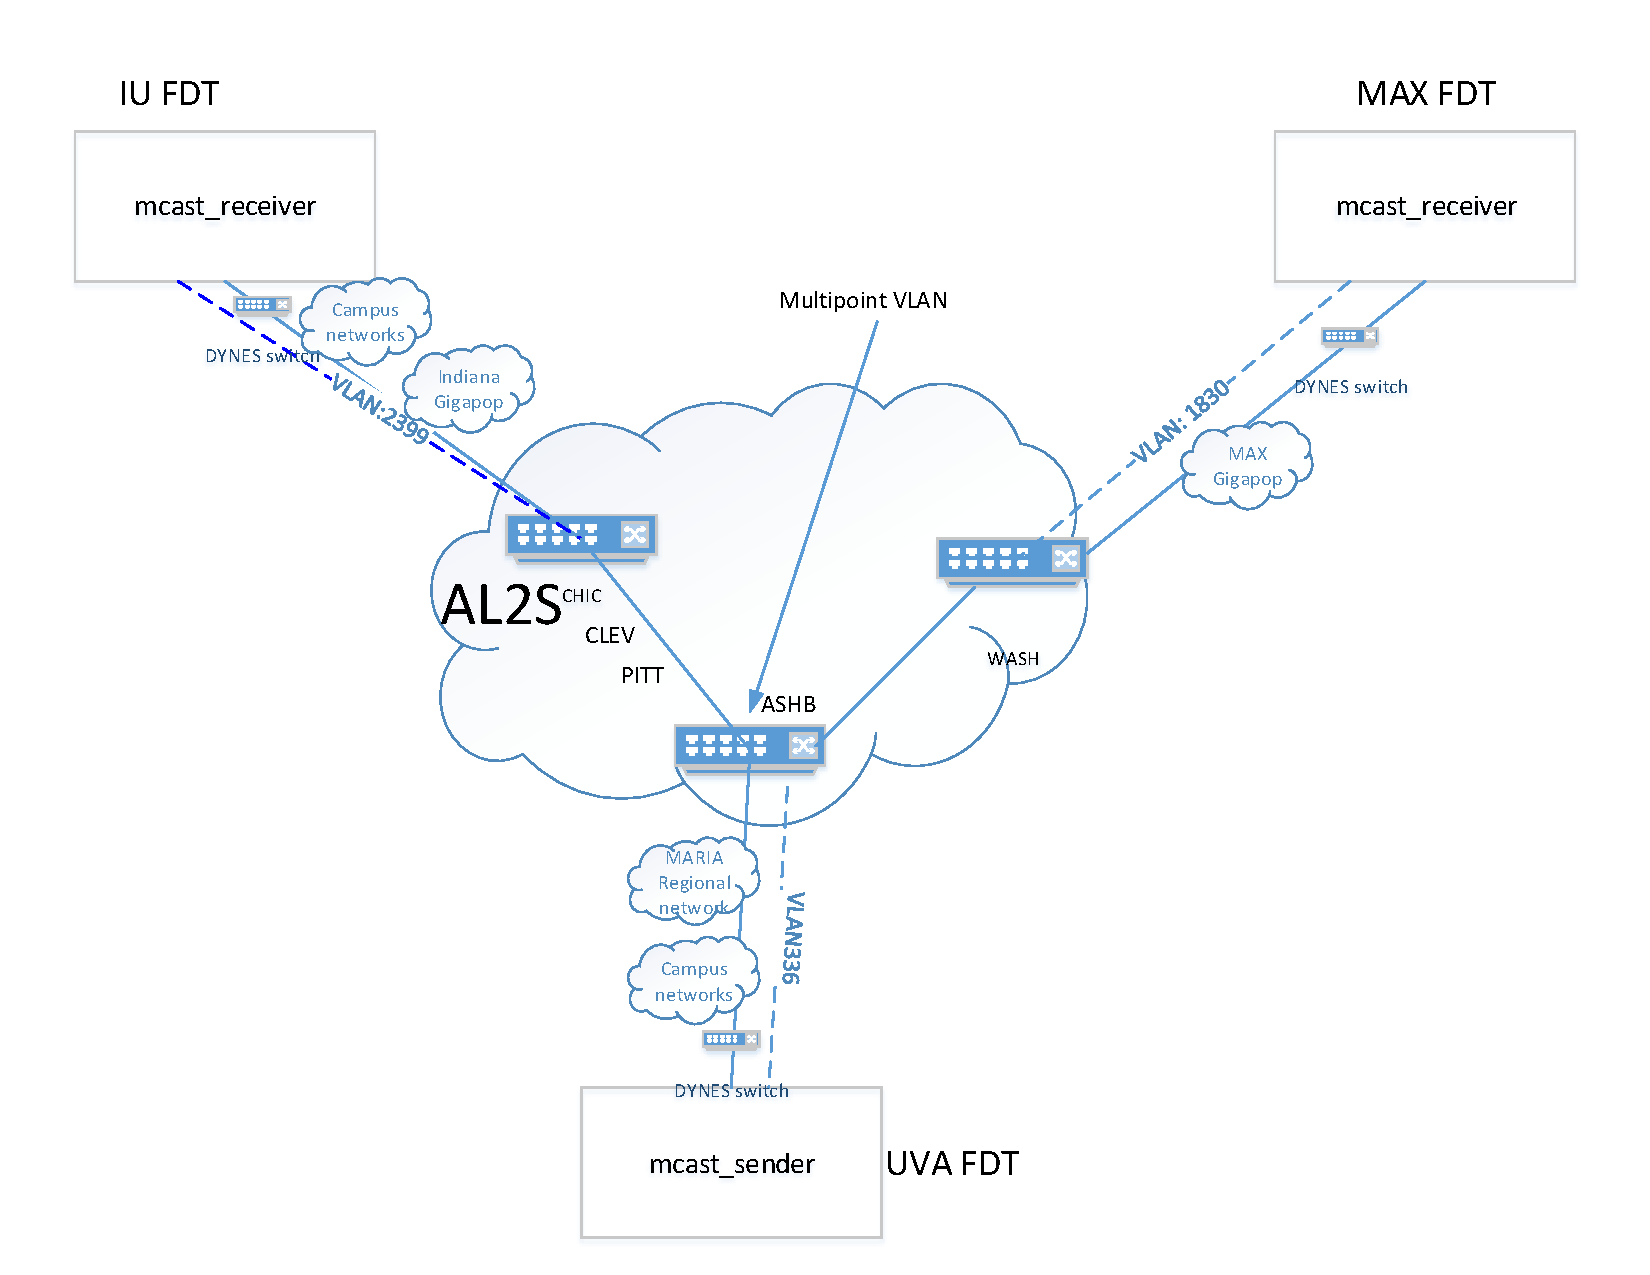
\includegraphics[width=0.8\textwidth]{figures/AL2S-mcast.pdf}
\caption{AL2S inter-domain multipoint circuit experiment}
\label{fig:wanmulticast}
\end{figure}

The second step consists of provisioning the intra-domain multipoint VLAN
across the Internet2 AL2S network as illustrated in Fig.~\ref{fig:oessal2s}.
Three endpoints are interconnected via this multipoint VLAN:
(i) MARIA's connection to interface \texttt{et-3/0/0.0} of Internet2 AL2S switch \texttt{sdn-sw.ashb.net.internet2.edu} (Ashburn, VA switch) with VLAN ID 336,
(ii) and MAX Gigapop's connection to interface \texttt{eth3/2} of Internet2 AL2S switch \texttt{sdn-sw.wash.net.internet2.edu} (McLean, VA switch) with VLAN ID 1830, (iii) and Indiana Gigapop's connection to interface \texttt{eth1/2} of Internet2 AL2S switch \texttt{sdn-sw.chic.net.internet2.edu} (Chicago, IL switch) with VLAN ID 2399.
\begin{figure}[htb!]
\centering
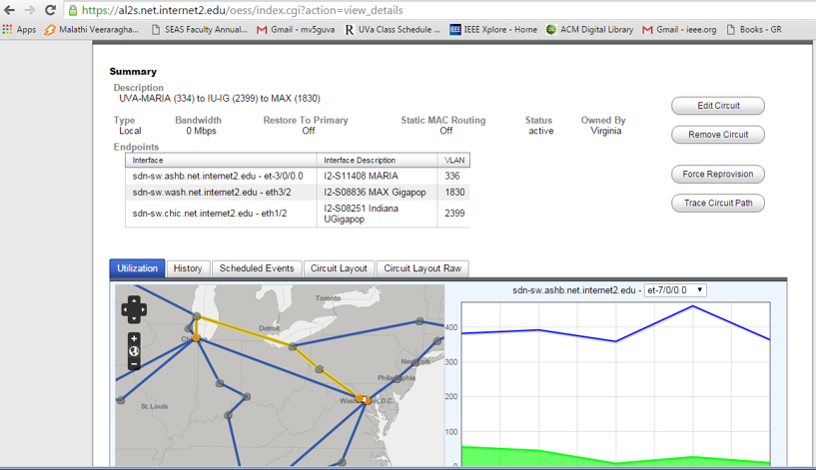
\includegraphics[width=0.8\textwidth]{figures/oess-AL2S.png}
\caption{AL2S OESS: Endpoints and VLAN selection}
\label{fig:oessal2s}
\end{figure}

The OpenFlow switch at the Internet2 AL2S Ashburn location is performing a complex function. 
For each VLAN-ID-336-tagged packet received on its port \texttt{et-3/0/0.0}, the Ashburn
switch makes two copies, and rewrites the VLAN ID in one copy to 2399 and to 1830 in the second copy.
The switch then sends the VLAN-ID-1830-tagged packet to port \texttt{et-1/3/0}, and sends VLAN-ID-2399-tagged packet to port \texttt{et-7/0/0}.
Similarly, each packet received with VLAN ID 2399 on port \texttt{eth1/2} in Internet2 AL2S Chicago switch is duplicated, and one copy is sent to Ashburn switch
with VLAN ID rewritten to 336, and the second copy is sent to Washington switch with VLAN ID rewritten to 1830,
and each packet received with VLAN ID 1830 on port \texttt{eth3/2} in AL2S Washington switch is duplicated with VLAN ID rewritten, and sent one copy with VLAN ID 336 to Ashburn and second copy with VLAN ID 2399 to Chicago switch.


As the Internet2 AL2S switches support only OpenFlow 1.0, it was surprising that these switches
support this complex copying and rewriting functionality. Nevertheless, this feature was
most useful for our multipoint VLAN provisioning.

\subsection{Data-Plane Experiments}
\label{sec:multipoint-data-plane}

The software used in these data-plane experiments consists of: (i) a multicast application for sending and receiving multicast traffic, (ii) Linux utility \texttt{vconfig} to configure VLAN IDs (tags) on host NICs,  (iii) Linux \texttt{ifconfig} to configure IP address and subnet mask for the configured VLAN, (iv) Linux utility \texttt{ping} to test the reachability on a VLAN, and (v) Linux utility \texttt{tcpdump} to capture multicast packets.

First, we describe a local (single-domain) multipoint experiment. Next, we present the results of
an inter-domain multipoint VLAN test.

\paragraph{Single-domain multipoint experiment}
\begin{figure}[htb!]
\centering
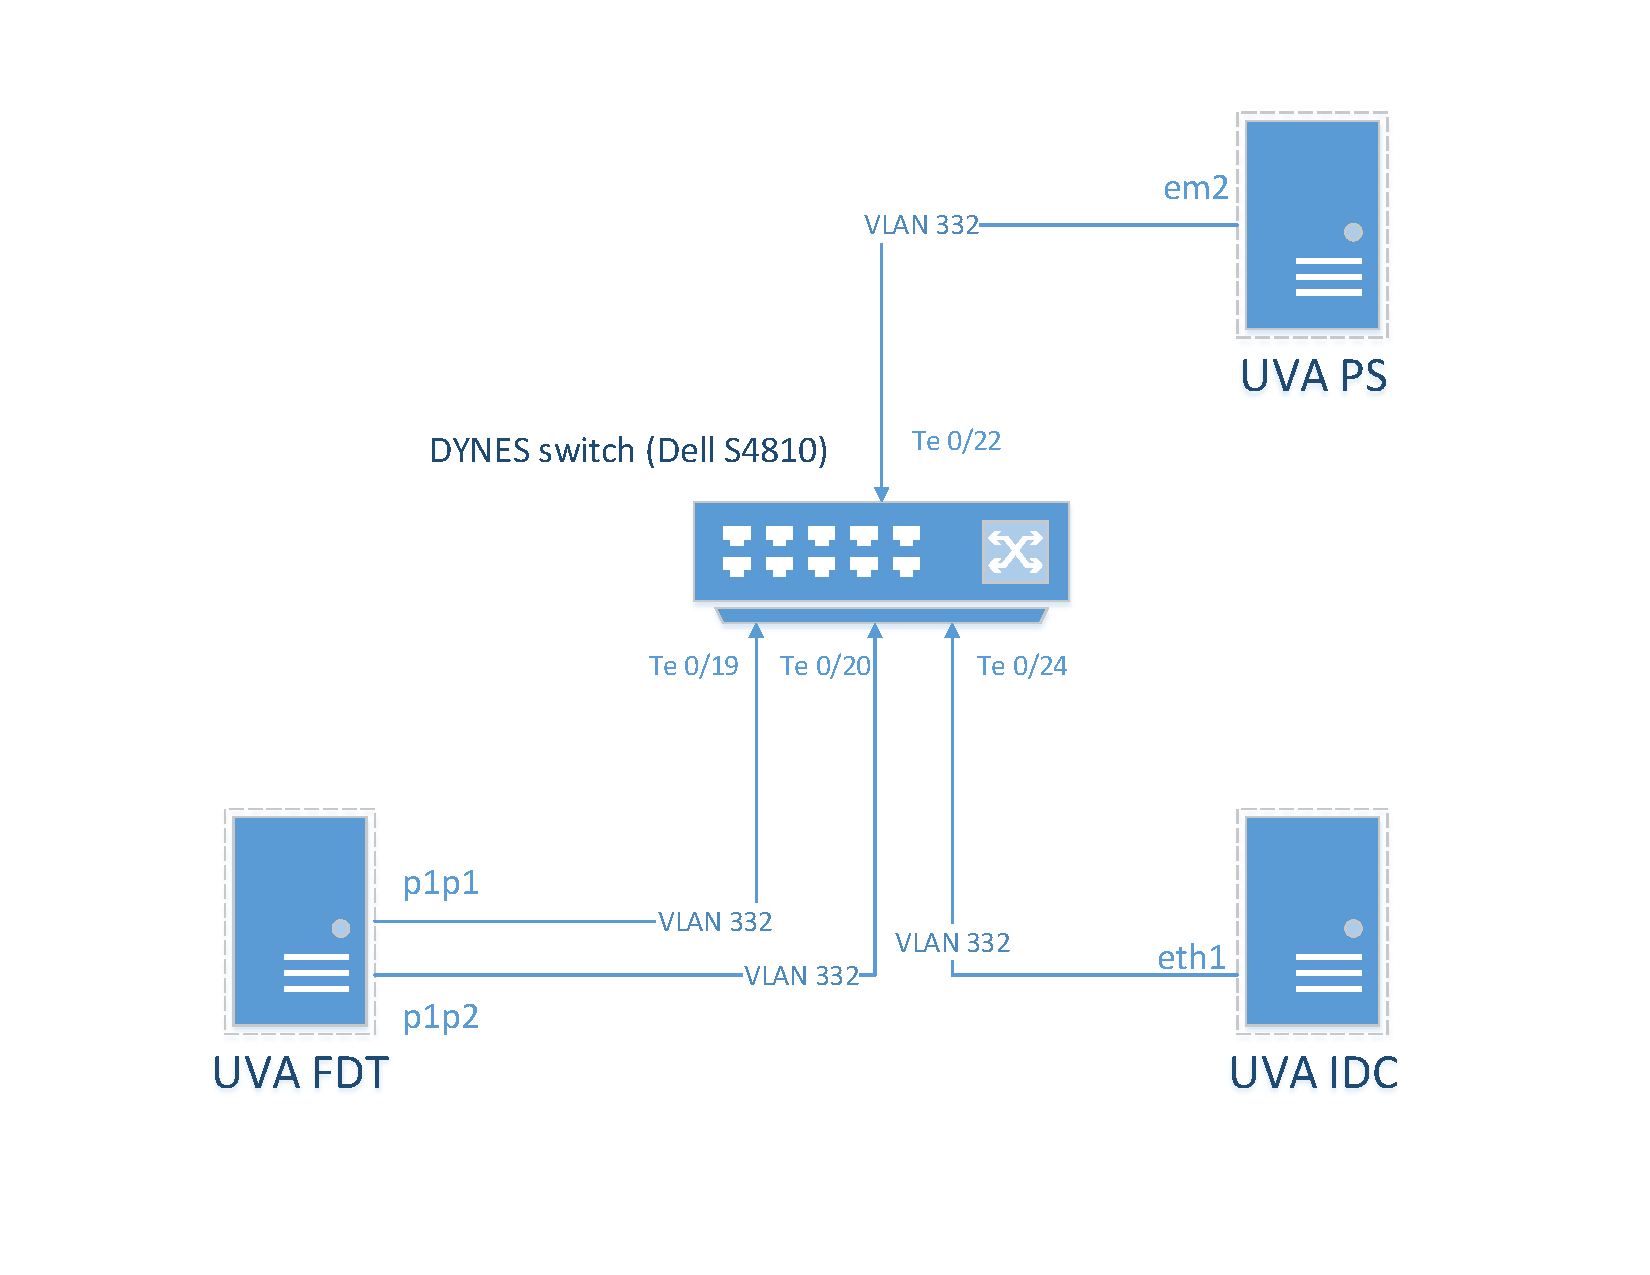
\includegraphics[width=0.8\textwidth]{figures/single-domain.pdf}
\caption{A local multipoint VLAN configuration through the UVA
DYNES switch connecting FDT, PS and IDC host}
\label{fig:single-domain}
\end{figure}

The multicast application was tested across an intra-domain multipoint VLAN. Fig.~\ref{fig:single-domain} shows the multipoint
VLAN configuration through the UVA DYNES switch connecting FDT, PS and IDC hosts. The same VLAN ID 332
is used on all three interfaces. The UVA DYNES switch, which is a Dell S4810 OpenFlow 1.0 switch, does not support multicasting
with VLAN ID rewrite, which implies that the same VLAN ID needs to be used on all interfaces.
This VLAN was created using OESS.
Fig.~\ref{fig:flowtable} shows one of the three OpenFlow flow-table entries created in the UVA DYNES switch by the OESS. When the switch receives a VLAN-332-tagged packet on port Te 0/19, the switch looks up the OpenFlow
table and finds a match for this packet with the entry shown in Fig.~\ref{fig:flowtable}. The switch then
replicates the packet, and sends one packet to each of three ports: Te 0/20, Te 0/22, Te 0/24. All three packets will be tagged with the same VLAN ID 332, as per the specifications of the OpenFlow flow-table entry
shown in Fig.~\ref{fig:flowtable}.

After the OpenFlow multipoint VLAN was set up via OESS, we configured VLANs at each of the three hosts
 using the process described in Section~\ref{sec:multidomain-SDN-FDT-access}. Private IP addresses on the same subnet were
 assigned to the VLANs at these hosts. Next, we used the \texttt{ping} utility to verify connectivity
 via this multipoint VLAN.

\begin{figure}[htb!]
\centering
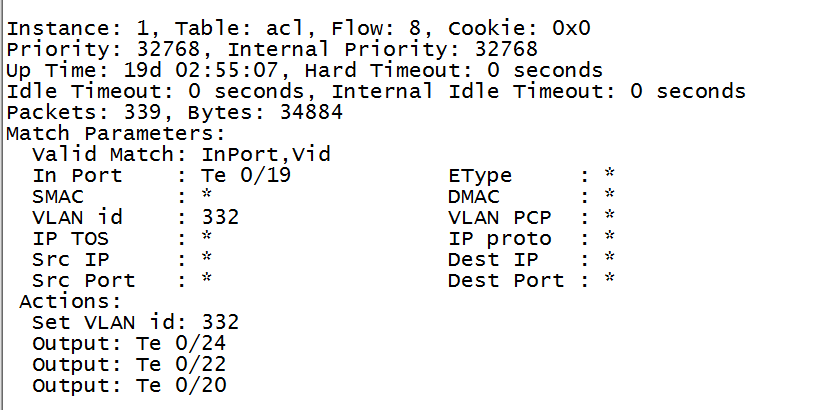
\includegraphics[width=0.8\textwidth]{figures/flow-table.png}
\caption{OpenFlow flow-table entry in the UVA DYNES switch}
\label{fig:flowtable}
\end{figure}

Second, a Linux multicast application was run to test the multipoint VLAN. The application
consists of a multicast sender (\texttt{mcast\_sender}) and a multicast receiver (\texttt{mcast\_receiver}).
We executed the \texttt{mcast\_sender} program on the UVA FDT, and the \texttt{mcast\_receiver} program
on the other two UVA DYNES hosts (IDC and PS).
As Fig.~\ref{fig:localmulticast} shows the unicast IP addresses of the VLAN at each host needs
to be specified as the first argument of both \texttt{mcast\_sender} and \texttt{mcast\_receiver}. These
IP addresses are 10.30.32.20 for the FDT NIC VLAN 332, 10.30.32.30 for the IDC NIC VLAN 332, and 
10.30.32.40 for the PS NIC VLAN 332. The specified unicast IP address is associated with the UDP socket
at each host that was opened with the \texttt{mcast\_sender} and \texttt{mcast\_receiver} using the multicast IP address 233.0.225.123 (which is the second argument). The last argument of both programs is the UDP port number 8888. 
Therefore, within the code, the second and third arguments are used to create a UDP socket. Then using
the Linux \texttt{setsockopt} system call, the unicast IP address provided as the first argument is associated
with the UDP socket. All datagrams passed to this UDP socket by the application are then sent to the interface
associated with the unicast IP address. The reason for associating a unicast IP address with the UDP socket that was created
with the multicast IP address is to avoid having to set an IP routing table entry corresponding
to the multicast IP address at the sending host. For example, if the sender has two NICs,
there could be an IP routing table entry for
the IP multicast address range to send packets to one of the two NICs, while the multipoint VLAN
could be configured to use the second NIC. In this case, either a new IP routing table entry is required
to direct packets addressed to the particular IP multicast address to the second NIC,
or the \texttt{setsockopt} function should be called by the application opening the multicast UDP socket
to associate the unicast IP address of the interface to which the multicast packets should be sent with that socket. In this case \texttt{mcast\_sender} and  \texttt{mcast\_receiver} perform the latter function. Since the unicast IP address provided is that of VLAN 332 in all
three hosts, all multicast packets will have a UDP header, an IP header with destination IP address set
to 233.0.225.123, an Ethernet header and an IEEE 802.1Q header with the VLAN ID set to 332. 
\begin{figure}[htb!]
\centering
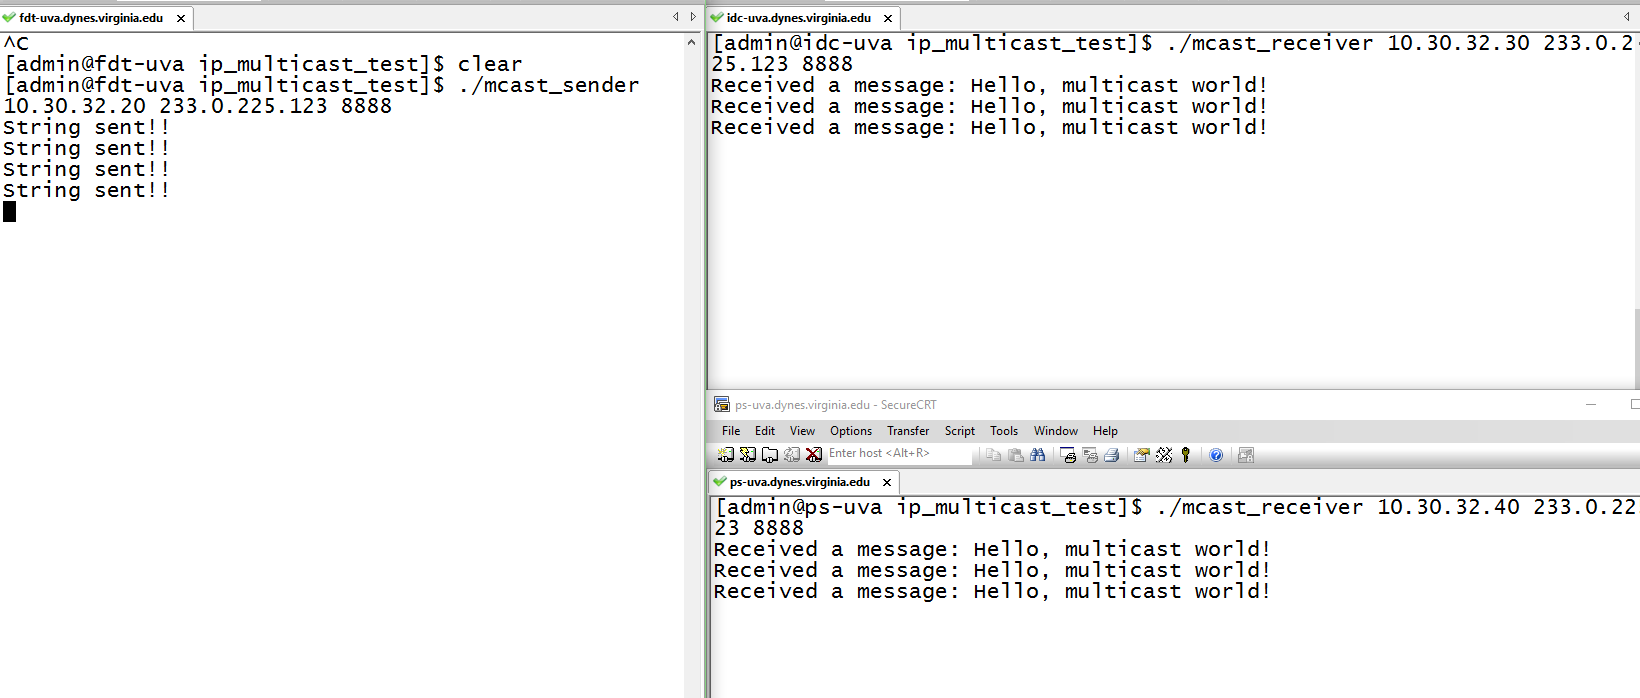
\includegraphics[width=0.8\textwidth]{figures/local-multicast.png}
\caption{Multicast application sending traffic from UVA FDT to UVA PS and UVA IDC hosts across a local multipoint VLAN}
\label{fig:localmulticast}
\end{figure}

The 233.0.225.123 IP address belongs to the 
GLOP range. The GLOP address IP range, 233.0.0.0/8, was assigned as an experimental address space for IP multicast service providers and networking researchers. The convention is to use the 16-bit autonomous system number (ASN)
in the second and third bytes. Since UVA's ASN is 225, the second and third bytes of our select multicast IP address 233.0.225.123 are 0 and 225, respectively.  

When the UVA FDT \texttt{mcast\_sender} program sent the message ``Hello, multicast world!'', the
\texttt{mcast\_receiver}  program running on the IDC and PS hosts received the message. However, when we changed the VLAN tags of these 3 interfaces to different values in local OESS, the related flow entries were not set in the flow table of UVA DYNES switch since multipoint VLAN tag translation feature was not supported in Dell  switch.
\begin{figure}[htb!]
\centering
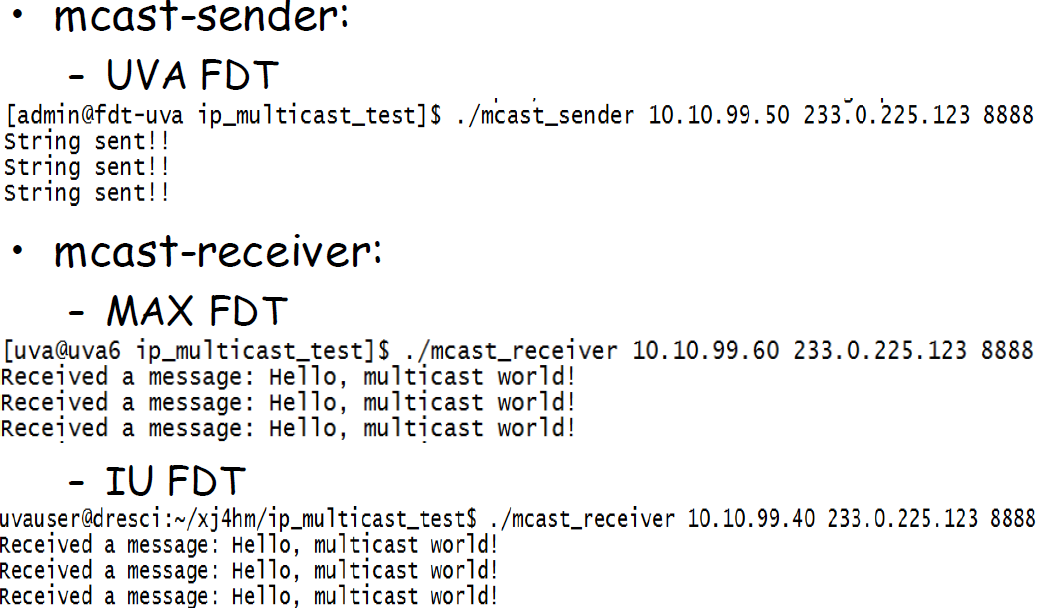
\includegraphics[width=0.8\textwidth]{figures/AL2Smulticast.png}
\caption{Multicast application sending traffic from UVA FDT to MAX FDT and IU FDT across an inter-domain multipoint VLAN}
\label{fig:widemulticast}
\end{figure}

\paragraph{Inter-domain multipoint experiment}
The control-plane actions for provisioning an inter-domain multipoint VLAN  were described in Section~\ref{sec:multipoint-control-plane}. These actions were executed to create a multipoint VLAN
between UVA FDT, MAX FDT and IU FDT. Specifically, this multipoint VLAN, with three different VLAN IDs, was illustrated
in Fig.~\ref{fig:oessal2s}.

The multicast application described above was then executed across this inter-domain multipoint VLAN. Fig.~\ref{fig:widemulticast} shows that the \texttt{mcast\_sender} program was executed at the UVA FDT,
and the \texttt{mcast\_receiver} program was executed at the MAX FDT and IU FDT. The ``Hello, multicast world!''
message sent by the \texttt{mcast\_sender} program running on the UVA FDT was successfully received by the 
\texttt{mcast\_receiver} processes at the MAX FDT and IU FDT.

\begin{figure}[htb!]
\centering
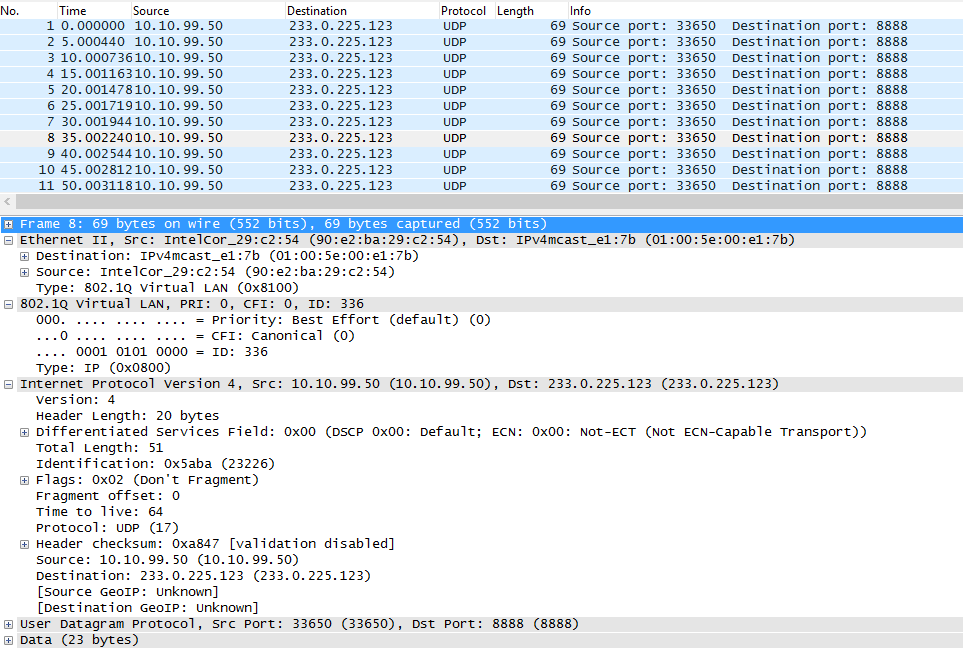
\includegraphics[width=0.8\textwidth]{figures/pcap.png}
\caption{Wireshark display of a pcap file}
\label{fig:multicast-pcap}
\end{figure}
To verify that packets were being multicast across the inter-domain multipoint VLAN, packets were captured with the \texttt{tcpdump} utility at the UVA FDT. Fig.~\ref{fig:multicast-pcap} shows some of the header fields, such as Source and Destination IP addresses, for the multicast packets. The source IP address is 10.10.99.50, which is the IP address assigned to VLAN 336 on the UVA FDT NIC, and the destination IP address is the GLOP IP address 233.0.225.123.
The destination MAC address of the Ethernet header, as seen in the lower window of Fig.~\ref{fig:multicast-pcap} is 01:00:5e:00:e1:7b, which is explained next.

Fig.~\ref{fig:mapping} shows the mapping solution used for multicast IP addresses. This solution is different
from the mapping procedure used for unicast IP addresses. To find the MAC address corresponding
to a unicast IP address, the Address Resolution Protocol (ARP) is used in which a request carrying the unicast
IP address being mapped is broadcast to all interfaces, and the interface whose IP address matches the address in the
request responds with its MAC address. However, for a multicast IP address, a single Ethernet MAC address
is required so that a single Ethernet frame, carrying the IP multicast packet, can be received by multiple receivers.
All multicast receiver NICs need to be configured with a multicast MAC address so that all these receivers will accept Ethernet frames whose destination MAC address matches the configured multicast MAC address. Without such a
multicast MAC address configuration, each  NIC will only accept Ethernet frames whose destination MAC address equals its own unicast MAC address and frames whose destination MAC address is 0xFF:FF:FF:FF:FF:FF (broadcast address). Therefore, when the \texttt{mcast\_sender} or \texttt{mcast\_receiver} program creates the \texttt{ipm} (IP-multicast) socket, the code calls the Ethernet driver to configure the NIC with another MAC address, 01:00:5e:00:e1:7b, so that the NIC accept accept frames with this destination MAC address. The Wireshark analysis of the captured packets verifies that this procedure
is being executed.
\begin{figure}[htb!]
\centering
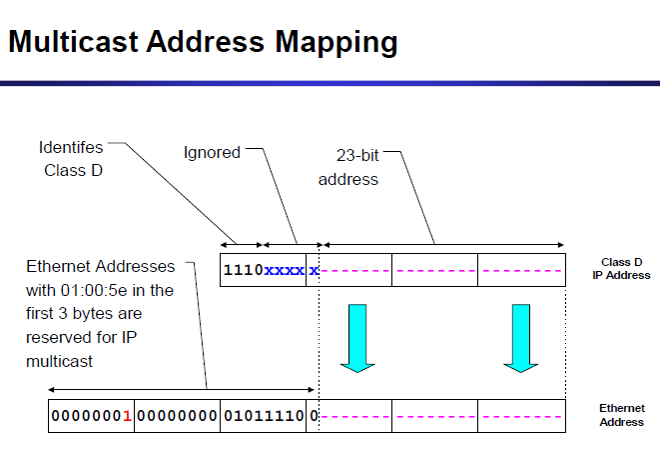
\includegraphics[width=0.8\textwidth]{figures/mapping.png}
\caption{Multicast IP address to multicast MAC address mapping}
\label{fig:mapping}
\end{figure}


\paragraph{Key Findings}
The key findings of the experiments are as follows: (i) multipoint VLANs that require VLAN ID translation (rewrite) is supported by at least some of the Internet2 AL2S switches, which allows for the creation of inter-domain multipoint VLAN. This finding is important for the deployment of LDM7, which was our motivating application to pursue SDN-controlled path-based networking in general, and multipoint VLANs in particular. (ii) Packets with the multicast destination IP address were dropped by firewalls in some campus networks and some regional networks. A systematic method is required for debugging connectivity across multiple domains.



\section{Related Work}
Multiple projects were started during the 2003-2006 time frame to address the issue of dynamic provisioning of path-based networking service within the REN community. This work was motivated by a desire to develop alternatives and enhancements to best-effort IP service for large-bandwith science data flows. These
include DOE funed OSCARS \cite{OSCARS}, UltraScience Net (USN) \cite{1541694}, TeraPaths \cite{4444698} and Lambda Station \cite{4374315} projects, and NSF Circuit-switched High-speed End-to-End Transport ArcHitecture (CHEETAH) \cite{1497551} and Dynamic Resource Allocation via GMPLS Optical Networks (DRAGON) \cite{4146687} projects. Further, an international
collaboration between Europe's GEANT\footnote{http://services.geant.net/bod/Pages/Home.aspx}, Japan's JGN-X\footnote{http://www.jgn.nict.go.jp/english/index.html}, Canada's CANARIE\footnote{http://www.canarie.ca/en/home},
and Brazil's RNP\footnote{http://www.rnp.br/en}, resulted in IDCP, which
is used in OSCARS. The objective was to provide both packet service, e.g., best-effort IP, and dynamic path networking service over a common infrasturcture with the control-plane intelligence. This objective has been realized in DOE's Energy Sciences Network (ESNet), Internet2 on their ION and AL2S networks, and increasingly on university campuses and regionals as illustrated in Fig.~\ref{fig:network}. 

The NSF Global Environment for Network Innovation (GENI) program\footnote{http://www.geni.net/} also supports the provisioning
of Layer-2 SDNs through OpenFlow-enabled or other switches.
Various controllers have been developed in the GENI program.
For example, GENI Network Stitching Architecture
allows for the creation of virtual network slices and virtual machines. Projects such as ProtoGENI\footnote{http://www.protogeni.net} and ExoGENI\footnote{http://www.exogeni.net} have developed proprietary multi-domain solutions to allocate internel network resources across their global footprints.
The GENI infrastructure spans many domains, a.k.a. aggregates, to support large-scale virtual networks. The GENI goal, which is to support network researchers,
is different from the goal of our multi-domain deployment,
which is to bring dynamic L2 path service into every-day use by university
scientists. This difference in goals allows for the use of a tree model
in GENI stitching unlike the daisy-chain model of OSCARS. In the tree
model, the client user needs to be independently authenticated by the aggregate managers controlling each domain. In contrast, the daisy-chain solution in OSCARS allows for a provider to have service-level agreements with neighbouring providers. Therefore, the OSCARS is more along the lines of the public switched telephone network and Internet, both of which successfully reached global scale.

\section{Conclusions}
This chapter described our experiences with deploying a multi-domain SDN and testing
a dynamic Layer-2 (L2) path service across this SDN. Our work demonstrated that inter-domain point-to-point
L2 paths can be created and released automatically, i.e., without administrator involvement, by using distributed per-domain SDN controllers. We offered insights into this complex deployment process
and identified modifications required to the protocols and controllers
for improving user experience and scalability of this dynamic L2 path service.
We also developed a methodology for provisioning inter-domain multipoint VLANs, and demonstrated
the successful use of these VLANs for a multicast application.

%%%Talk about the multipoint VLAN 

\chapter{Conclusions and Future Work}
\label{sec:conclusion}

This thesis identified an exciting new problem
of rate determination for L2 multipoint virtual topologies
to serve variable-rate file streams to multiple receivers. Prior work
on rate computation methods were designed for audio/video
streams, not file streams. The problem is based on the need
for scalability in a real deployment as data volumes and
number of receivers have grown. Our solution was based, not
on models, but on actual traffic characteristics. These
characteristics, such as right-skewed file size and file
inter-arrival times, and variability from day-to-day,
are likely to hold for other types of file-streams.
Our solution, based on an empirical method and an exponential weighted moving average scheme, could therefore have wide applicability.
Evaluation of our method with real traffic showed that
while throughput constraints can be met by selecting a suitably high
rate, utilization varies based on the burstiness of the file stream.
However, if rate-guaranteed Layer-2 services are offered
on the same network as best-effort IP services, and packet schedulers
are configured to operate in work-conserving mode, the utilization levels
of the L2 multipoint topologies are not of concern. 
We also found that for this application, required rates are only on
the order of Mbps, which is a small fraction of current-day Gb/s networks.

The thesis also described our experience in deploying a multi-domain SDN and testing
a dynamic Layer-2 (L2) path service across this SDN. Our work demonstrated that inter-domain L2 paths can be created and released automatically, i.e., without administrator involvement, by using distributed per-domain SDN controllers.
We offered insights into this complex deployment process
and identified modifications required to the protocols and controllers
for improved user experience and scalability of this dynamic L2 path service. We also developed a methodology for provisioning inter-domain multipoint VLANs, and demonstrated
the successful use of these VLANs for a multicast application. Lessons learned include an understanding of the equipment
and configuration steps required to enable dynamic L2 service in each domain, and an understanding of how to configure end-hosts to run existing applications, without modifications, across end-to-end L2 paths. We developed methods for debugging path-setup failures, and identified
areas of improvement required in the controllers and in the administrative processes.

Future work items include the (i) design and implementation of diagnostic tools to debug connectivity failures on VLANs, (ii) characterization of the rate at which feedtrees (the set of LDM servers subscribed to a feedtype) change in order to determine how often L2 multipoint VLANs would need modifications, and (iii) incorporation of an OESS client into LDM7 to enable the upstream LDM server to submit requests to OESS to dynamically create a new multipoint VLAN for a feedtype, release an existing multipoint VLAN if all subscriptions to a feedtype end, to add a provisioned VLAN segment from a downstream LDM7 server to an AL2S switch into an existing L2 multipoint VLAN across AL2S if a receiver subscribes a new feedtype, and to delete a provisioned VLAN segment when a downstream LDM7 server drops a subscription to a feedtype.












\appendix

\chapter{Appendix}

\section{Characterization of IDD feedtypes}

In Table.~\ref{tab:size-summary} and Table.~\ref{tab:inter-arr-time-summary}, we listed several quantiles of size and inter-arrival time of top five feedtypes.
In this appendix, we provide the histograms of size and inter-arrival time for the other 4 feedtypes (NGRID, NEXRAD2, NEXRAD3, FSL2).

\begin{figure}[htb!]
\centering
    \begin{subfigure}{0.5\linewidth}
        \centering
        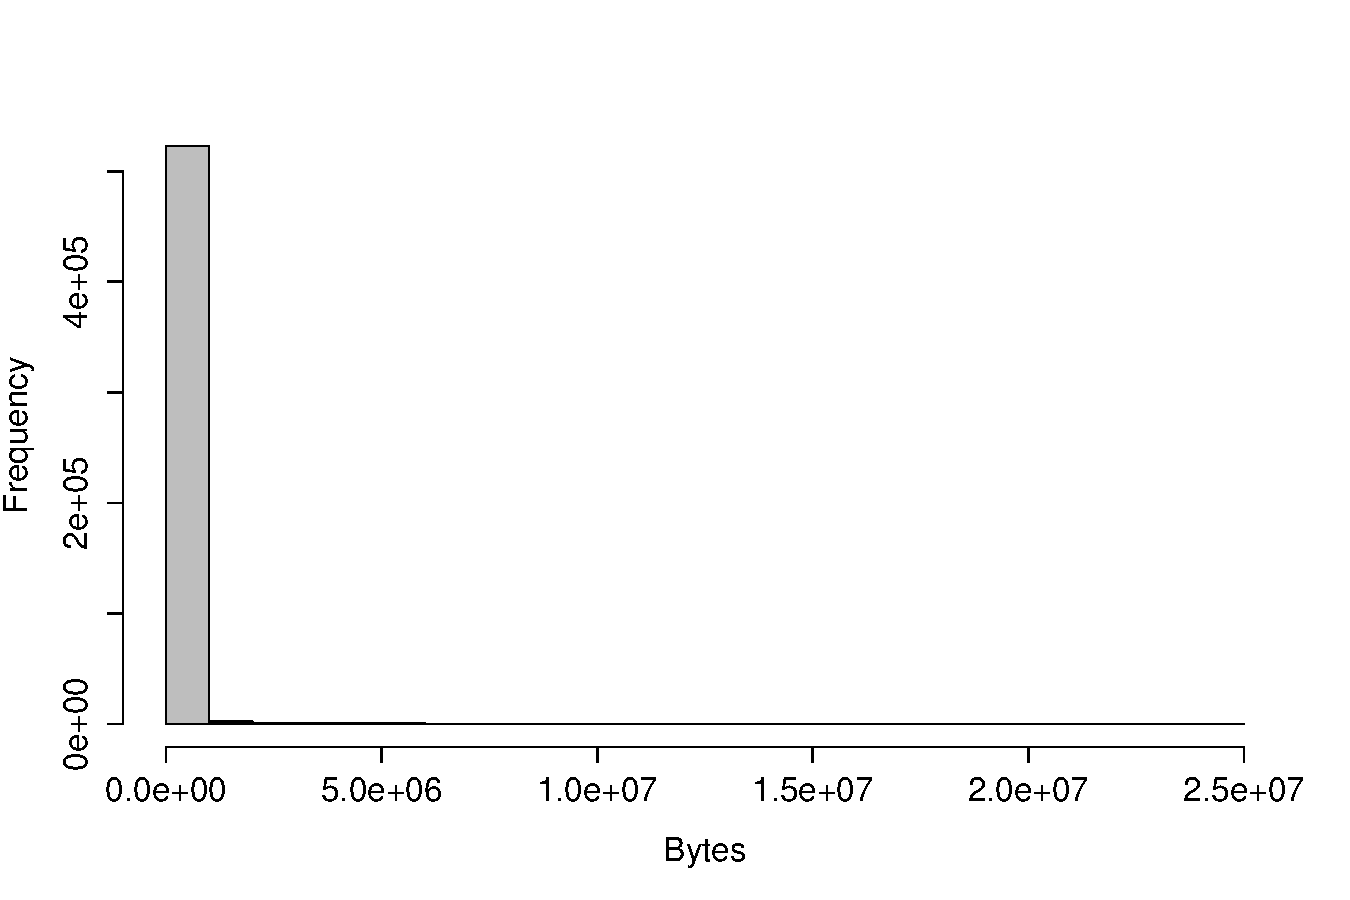
\includegraphics[width=2.2in]{figures/Size-hist-NGRID0602.pdf}
        \caption{Whole size range}
        \label{NGRID_Size_Whole}
    \end{subfigure}\hfill
    \begin{subfigure}{0.5\linewidth}
	\centering
    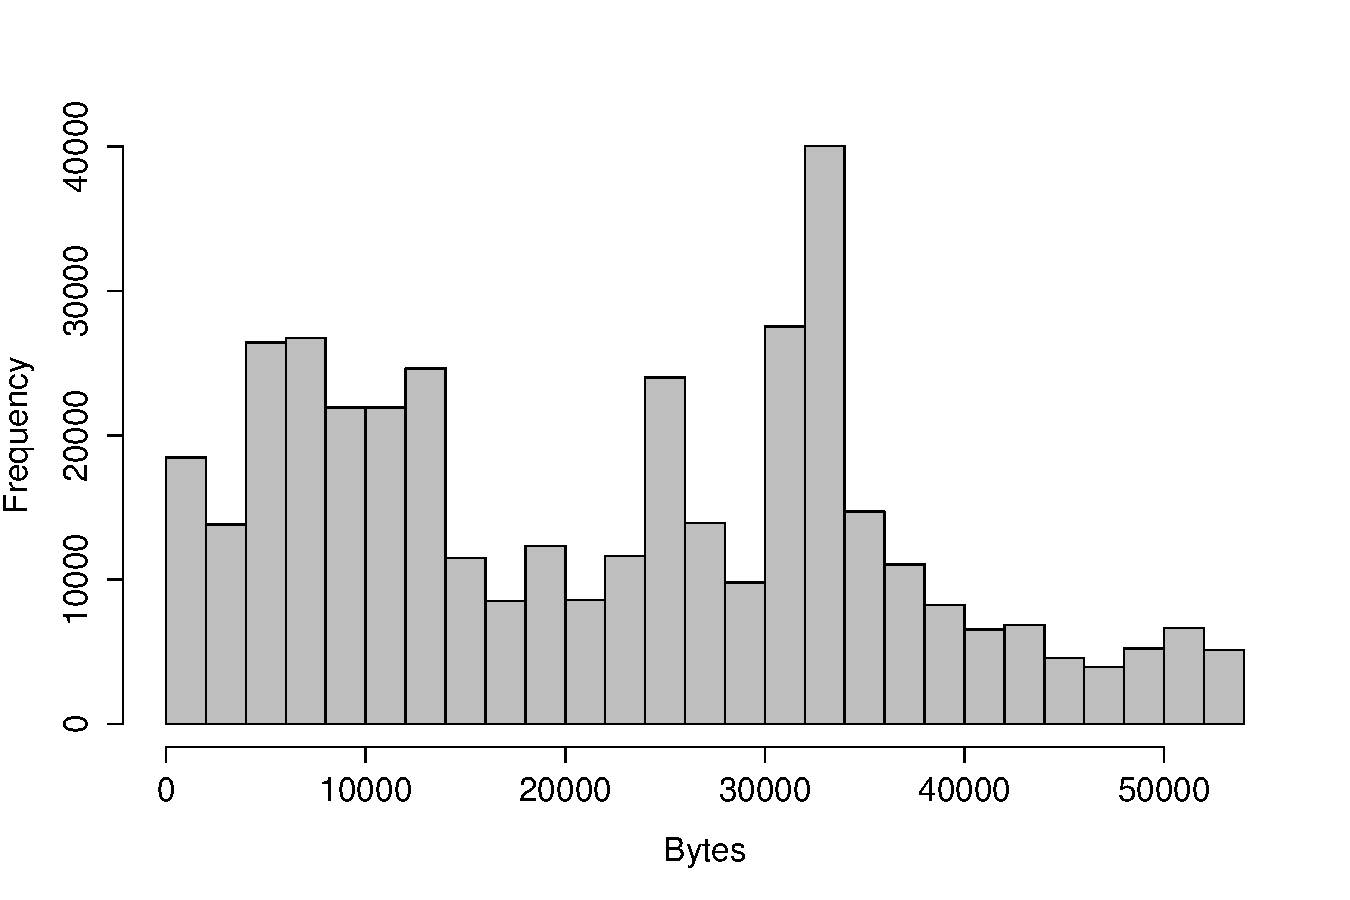
\includegraphics[width=2.2in]{figures/Size-hist-NGRID602-TOP75.pdf}
    %\includegraphics[width=3.5in]{figures/CONDUIT-size-75.eps}
        \caption{Top 75 percentile of size range}
        \label{NGRID_Size_75}
    \end{subfigure}\hfill
    \caption{NGRID feedtype, histograms of the size of the data products sent on June 02, 2014}
    \label{NGRID_Size}
\end{figure}

NGRID (NG) \cite{NGRID} feedtype is grided data from National Oceanic and Atospheric Administration (NOAA). Fig.~\ref{NGRID_Size} shows that almost 75\% data products are smaller than 50KB. Fig.~\ref{NG_time} shows that most of the inter-arrival time are less than 20ms.

\begin{figure}[htb!]
\centering
    \begin{subfigure}{0.5\linewidth}
        \centering
        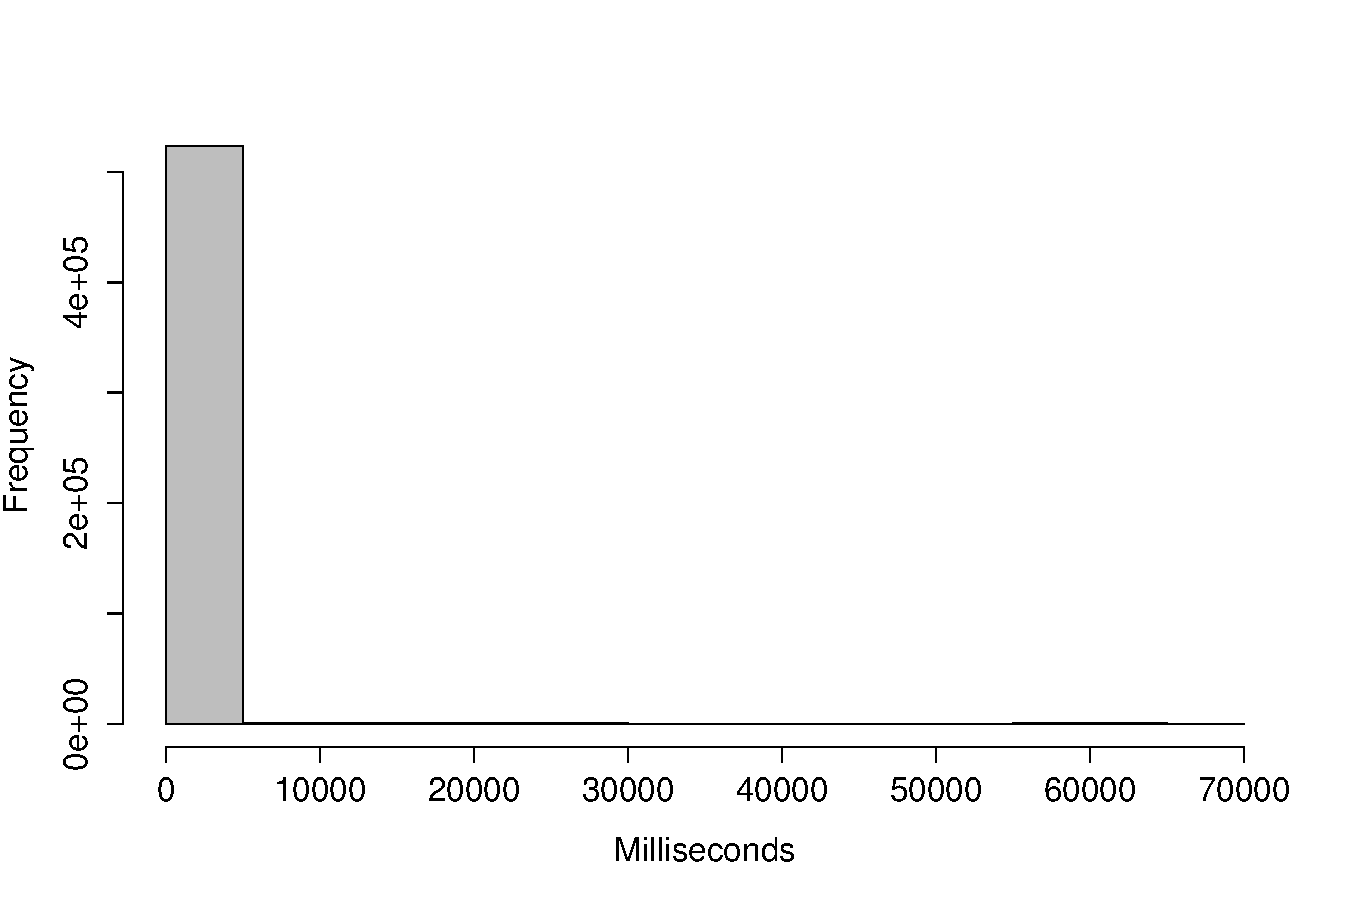
\includegraphics[width=2.2in]{figures/Inter-hist-NGRID0602.pdf}
        %\includegraphics[width=3.5in]{figures/CONDUIT_Size.eps}
        \caption{Whole inter-arrival time range}
        \label{NGRID_Inter_Whole}
    \end{subfigure}\hfill
    \begin{subfigure}{0.5\linewidth}
	\centering
    \includegraphics[width=2.2in]{figures/Inter-hist-NGRID0602-TOP75.pdf}
    %\includegraphics[width=3.5in]{figures/CONDUIT-size-75.eps}
        \caption{Top 75 percentile of inter-arrival time range}
        \label{NGRID_Inter_75}
    \end{subfigure}\hfill
    \caption{NGRID feedtype, histograms of inter-arrival time of data products sent on June 02, 2014, }
    \label{NG_time}
\end{figure}

%NEXRAD2-5
\begin{figure}[htb!]
\centering
    \begin{subfigure}{0.5\linewidth}
        \centering
        \includegraphics[width=2.2in]{figures/size-hist-NEXRAD20602.pdf}
        %\includegraphics[width=3.5in]{figures/CONDUIT_Size.eps}
        \caption{Whole size range }
        \label{NEXRAD2_Size_Whole}
    \end{subfigure}\hfill
    \begin{subfigure}{0.5\linewidth}
	\centering
    \includegraphics[width=2.2in]{figures/size-hist-NEXRAD20602-TOP75.pdf}
    %\includegraphics[width=3.5in]{figures/CONDUIT-size-75.eps}
        \caption{Top 75 percentile of size range}
        \label{NEXRAD2_Size_75}
    \end{subfigure}\hfill
    \caption{NEXRAD2 feedtype, histograms of size of data products sent on June 02, 2014}
    \label{NEXRAD2_Size}
\end{figure}

NEXRAD2 feedtype is NEXRAD level II radar data. Fig.~\ref{NEXRAD2_Size} shows the file size of this type of data is large. The top 75\% size histogram Fig.~\ref{NEXRAD2_Size_75} indicates that most of the size of data products are within 40KB.

\begin{figure}[htb!]
\centering
    \begin{subfigure}{0.5\linewidth}
        \centering
        \includegraphics[width=2.2in]{figures/Inter-hist-NEXRAD20602.pdf}
        %\includegraphics[width=3.5in]{figures/CONDUIT_Size.eps}
        \caption{Whole inter-arrival time range}
        \label{NEXRAD2_Inter_Whole}
    \end{subfigure}\hfill
    \begin{subfigure}{0.5\linewidth}
	\centering
    \includegraphics[width=2.2in]{figures/Inter-hist-NEXRAD20602-TOP75.pdf}
    %\includegraphics[width=3.5in]{figures/CONDUIT-size-75.eps}
        \caption{Top 75 percentile of inter-arrival time range}
        \label{NEXRAD2_Inter_75}
    \end{subfigure}\hfill
    \caption{NEXRAD2 feedtype, histograms of inter-arrival time of data products sent on June 02, 2014}
    \label{NEXRAD2_time}
\end{figure}

%NEXRAD3
\begin{figure}[htb!]
\centering
    \begin{subfigure}{0.5\linewidth}
        \centering
        \includegraphics[width=2.2in]{figures/size-hist-NEXRAD30602.pdf}
        %\includegraphics[width=3.5in]{figures/CONDUIT_Size.eps}
        \caption{Whole size range}
        \label{NEXRAD3_Size_Whole}
    \end{subfigure}\hfill
    \begin{subfigure}{0.5\linewidth}
	\centering
    \includegraphics[width=2.2in]{figures/size-hist-NEXRAD30602-TOP75.pdf}
    %\includegraphics[width=3.5in]{figures/CONDUIT-size-75.eps}
        \caption{Top 75 percentile of size range}
        \label{NEXRAD3_Size_75}
    \end{subfigure}\hfill
    \caption{NEXRAD3 feedtype, histogram of size of data products sent on June 02, 2014}
    \label{NEXRAD3_Size}
\end{figure}

NEXRAD3 \cite{NEXRAD3} feedtype is NEXRAD level III data. Fig.~\ref{NEXRAD3_Size} indicates that the pattern of this feedtype is similar to NEXRAD2. Its file size is big with an average of 7 KB.

\begin{figure}[htb!]
\centering
    \begin{subfigure}{0.5\linewidth}
        \centering
        \includegraphics[width=2.2in]{figures/Inter-hist-NEXRAD30602.pdf}
        %\includegraphics[width=3.5in]{figures/CONDUIT_Size.eps}
        \caption{Whole inter-arrival time range}
        \label{NEXRAD3_Inter_Whole}
    \end{subfigure}\hfill
    \begin{subfigure}{0.5\linewidth}
	\centering
    \includegraphics[width=2.2in]{figures/Inter-hist-NEXRAD30602-TOP75.pdf}
    %\includegraphics[width=3.5in]{figures/CONDUIT-size-75.eps}
        \caption{Top 75 percentile of inter-arrival time range}
        \label{NEXRAD3_Inter_75}
    \end{subfigure}\hfill
    \caption{NEXRAD3 feedtype, histograms of inter-arrival time of data products sent on June 02, 2014}
    \label{NEXRAD3_time}
\end{figure}

Fig.~\ref{NEXRAD3_time} shows that the inter-arrival time of NEXRAD3 is small, which means NEXRAD3 data products are distributed with a high frequency. The top 75\% inter-arrival time histogram Fig.~\ref{NEXRAD3_Inter_75} shows most of the data arrive within 10 millisecond after the previous one.

%FSL2
\begin{figure}[htb!]
\centering
    \begin{subfigure}{0.5\linewidth}
        \centering
        \includegraphics[width=2.2in]{figures/size-hist-FSL20602.pdf}
        %\includegraphics[width=3.5in]{figures/CONDUIT_Size.eps}
        \caption{Whole size range}
        \label{FSL2_Size_Whole}
    \end{subfigure}\hfill
    \begin{subfigure}{0.5\linewidth}
	\centering
    \includegraphics[width=2.2in]{figures/size-hist-FSL20602-TOP75.pdf}
    %\includegraphics[width=3.5in]{figures/CONDUIT-size-75.eps}
        \caption{Top 75 percentile of size range }
        \label{FSL2_Size_75}
    \end{subfigure}\hfill
    \caption{FSL2 feedtype, histogram of size of data products sent on June 02, 2014}
    \label{FSL2_Size}
\end{figure}

FSL2 feedtype \cite{FSL2} is NOAA Profiler Network-Forecast Systems Laboratory data, which is wind profiler data. Fig.~\ref{FSL2_Size} shows that the data size is large, usually 1MB for each data product.

\begin{figure}[htb!]
\centering
    \begin{subfigure}{0.5\linewidth}
        \centering
        \includegraphics[width=2.2in]{figures/Inter-hist-FSL20602.pdf}
        %\includegraphics[width=3.5in]{figures/CONDUIT_Size.eps}
        \caption{Whole inter-arrival time range }
        \label{FSL2_Inter_Whole}
    \end{subfigure}\hfill
    \begin{subfigure}{0.5\linewidth}
	\centering
    \includegraphics[width=2.2in]{figures/Inter-hist-FSL20602-TOP75.pdf}
    %\includegraphics[width=3.5in]{figures/CONDUIT-size-75.eps}
        \caption{Top 75 percentile of inter-arrival time range  }
        \label{FSL2_Inter_75}
    \end{subfigure}\hfill
    \caption{FSL2 feedtype, histogram of inter-arrival time of data products sent on June 02, 2014}
    \label{FSL2_time}
\end{figure}


\begin{figure}[htb!]
\centering
    \begin{subfigure}{0.5\linewidth}
        \centering
        \includegraphics[width=2.2in]{figures/rate_time_NEXRAD20602.pdf}
        %\includegraphics[width=3.5in]{figures/CONDUIT_Size.eps}
        \caption{NEXRAD2 feedtype}
        \label{fig:N2-rate}
    \end{subfigure}\hfill
    \begin{subfigure}{0.5\linewidth}
	\centering
    \includegraphics[width=2.2in]{figures/rate_time_NEXRAD30602.pdf}
    %\includegraphics[width=3.5in]{figures/CONDUIT-size-75.eps}
        \caption{NEXRAD3 feedtype}
        \label{fig:N3-rate}
    \end{subfigure}\hfill
    \caption{Rate vs. time of NEXRAD2 and NEXRAD3 feedtypes}
    \label{NEXRAD-rate}
\end{figure}

Fig.~\ref{NEXRAD-rate} shows that the data products arrival pattern of NEXRAD2 is similar to the pattern of NEXRAD3, but the arrival rate of NEXRAD2 is higher than that of NEXRAD3. Both NEXRAD2 and NEXRAD3 feedtypes have high throughput. 


\begin{figure}[htb!]
\centering
\includegraphics[width=2.2in]{figures/rate_time_FSL20602.pdf}
\caption{FSL2 feedtype}
\label{fig:FSL2-rate}
\end{figure}

Fig.~\ref{fig:FSL2-rate} shows that FSL2 feedtype consists of big-size files. It also indicates that the FSL2 data arrival rate has a periodicity about 1 hour.

% \section{Rate prediction method for SDN software}

% Follow the software guidance, software architecture graph,  

% For each program,
% Describe the language in which the program was written.
% Give name of program. State what input file the program is reading. What is the main purpose of the program? What output file is it creating?


%\section{LDM performance measurement software}




\backmatter
\chapter*{Acknowledgments} 

I would like to take this opportunity to thank many people without whom this thesis would not have been possible.  First of all, I would like to thank my advisor Professor Veeraraghavan, who is always so brilliant and responsible. When I first came to UVa to start my graduate career, this research area was a whole new world for me. Professor Veeraraghavan was always so patient and supportive. She taught me not only knowledge in this networking area, but also the way to conduct research and tackle problems which I believe would be beneficial throughout my career and life. She helped me identify and develop a strong interest in computer networks research. Most importantly, her support and guidance helped me accumulate confidence along the way and realize what I am capable of. I would also like to thank my committee members, Professor Dugan and Professor Qi for taking the time to review my thesis and provide great suggestions.

This work was supported by NSF grants CNS-1116081,
OCI-1127340, ACI-1340910, and CNS-1405171, and the U.S.
Department of Energy (DOE) grant DE-SC0007341. I would like to thank our CC-NIE project Program Manager Kevin Thompson for giving me this opportunity to conduct networking research. 

I am fortunate to have a group of good colleagues and friends around me. I want to thank Fatemah Alali, Xiaoyu Wang, Sourav Maji, Fabrice Mizero, Gholamreza Rahimi, and Shawn Chen, they are smart, pleasant, and inspiring. We went through a lot of tough times together. Their great company has made graduate life much more fun and enjoyable. I sincerely wish them luck and success in future career, wherever they may be.

I want to thank UVA alumni students Yicheng Liang, Scott Tepsuporn and Xin Song for their contributions in this project. Without their help, these paper won't be published so successfully.

Moreover, I would like to thank our collaborators Steve Emmerson, Brian Cashman and Joseph Slezak. Your help and contributions really inspired me and played a significant role in this research project. I also would like to thank Chin Guok and AJ Ragusa for OSCARS and OESS input in Chapter.~\ref{sec:DYNES}.

Lastly, I want to thank my family without whom I cannot imagine what life would be like. Thanks for always supporting me and bringing me so many resources. I wish them good health and happiness all the time.





\ifwww
\else
\addcontentsline{toc}{chapter}{Bibliography}
\fi
\bibliographystyle{IEEEtran}
\bibliography{refs,IEEEabrv,References,base-refs,rfc}





\end{document}

